%% abtex2-modelo-trabalho-academico.tex, v-1.9.7 laurocesar
%% Copyright 2012-2018 by abnTeX2 group at http://www.abntex.net.br/ 
%%
%% This work may be distributed and/or modified under the
%% conditions of the LaTeX Project Public License, either version 1.3
%% of this license or (at your option) any later version.
%% The latest version of this license is in
%%   http://www.latex-project.org/lppl.txt
%% and version 1.3 or later is part of all distributions of LaTeX
%% version 2005/12/01 or later.
%%
%% This work has the LPPL maintenance status `maintained'.
%% 
%% The Current Maintainer of this work is the abnTeX2 team, led
%% by Lauro César Araujo. Further information are available on 
%% http://www.abntex.net.br/
%%
%% This work consists of the files abntex2-modelo-trabalho-academico.tex,
%% abntex2-modelo-include-comandos and abntex2-modelo-references.bib
%%

% ------------------------------------------------------------------------
% ------------------------------------------------------------------------
% abnTeX2: Modelo de Trabalho Academico (tese de doutorado, dissertacao de
% mestrado e trabalhos monograficos em geral) em conformidade com 
% ABNT NBR 14724:2011: Informacao e documentacao - Trabalhos academicos -
% Apresentacao
% ------------------------------------------------------------------------
% ------------------------------------------------------------------------

\documentclass[
	% -- opções da classe memoir --
	12pt,				% tamanho da fonte
	openright,			% capítulos começam em pág ímpar (insere página vazia caso preciso)
	twoside,			% para impressão em recto e verso. Oposto a oneside
	a4paper,			% tamanho do papel. 
	% -- opções da classe abntex2 --
	%chapter=TITLE,		% títulos de capítulos convertidos em letras maiúsculas
	%section=TITLE,		% títulos de seções convertidos em letras maiúsculas
	%subsection=TITLE,	% títulos de subseções convertidos em letras maiúsculas
	%subsubsection=TITLE,% títulos de subsubseções convertidos em letras maiúsculas
	% -- opções do pacote babel --
	english,			% idioma adicional para hifenização
	%french,				% idioma adicional para hifenização
	%spanish,			% idioma adicional para hifenização
	brazil				% o último idioma é o principal do documento
	]{abntex2}

% ---
% Pacotes básicos 
% ---
\usepackage{lmodern}			% Usa a fonte Latin Modern			
\usepackage[T1]{fontenc}		% Selecao de codigos de fonte.
\usepackage[utf8]{inputenc}		% Codificacao do documento (conversão automática dos acentos)
\usepackage{indentfirst}		% Indenta o primeiro parágrafo de cada seção.
\usepackage{color}				% Controle das cores
\usepackage{graphicx}			% Inclusão de gráficos
\usepackage{microtype} 			% para melhorias de justificação
% ---
		
% ---
% Pacotes adicionais, usados apenas no âmbito do Modelo Canônico do abnteX2
% ---
\usepackage{lipsum}				% para geração de dummy text
% ---

% ---
% Pacotes de citações
% ---
\usepackage[brazilian,hyperpageref]{backref}	 % Paginas com as citações na bibl
\usepackage[alf, abnt-emphasize=bf]{abntex2cite}	% Citações padrão ABNT

% --- 
% CONFIGURAÇÕES DE PACOTES
% --- 

% ---
% Configurações do pacote backref
% Usado sem a opção hyperpageref de backref
%\renewcommand{\backrefpagesname}{Citado na(s) página(s):~}
\renewcommand{\backrefpagesname}{}
% Texto padrão antes do número das páginas
\renewcommand{\backref}{}
% Define os textos da citação
%\renewcommand*{\backrefalt}[4]{
%	\ifcase #1 %
%		Nenhuma citação no texto.%
%	\or
%		Citado na página #2.%
%	\else
%		Citado #1 vezes nas páginas #2.%
%	\fi}%
\renewcommand*{\backrefalt}[4]{}%
% workaround referências a anexos
\newcommand{\refanexo}[1]{\hyperref[#1]{Anexo~\ref{#1}}}
% --- Pacote próprios
\usepackage{amsmath}
\usepackage{amsfonts}
\usepackage{amssymb}
\usepackage{bm}
\usepackage{bbm}
\usepackage{mathrsfs}
%\usepackage{graphicx}
%\usepackage{float}
\usepackage{url}
\usepackage{verbatim}
\usepackage{babel}
\usepackage{subcaption}
\usepackage[portuguesekw, boxed]{algorithm2e}
\usepackage[font=small,labelfont=bf]{caption}
% --- 
% --- Configurações extras
% Acerta nomes dos algoritmos
\SetAlgorithmName{Algoritmo}{Algoritmo}{Lista de algoritmos}
% ---
% Informações de dados para CAPA e FOLHA DE ROSTO
% ---
\titulo{Algoritmos Genéticos\\Um algoritmo evolucionário para otimização}
\autor{Fabricio Kassardjian}
\local{Brasil}
\data{\today}
\orientador{Anatoli Iambartsev}
\instituicao{%
  Universidade de São Paulo -- USP
  \par
  Insituto de Matemática e Estatística
  \par
  Bacharelado em Matemática Aplicada e Computacional}
\tipotrabalho{Monografia}
% O preambulo deve conter o tipo do trabalho, o objetivo, 
% o nome da instituição e a área de concentração 
\preambulo{Monografia de final de curso, Instuto de Matemática e Estatística - USP, Matemática Aplicada}
% ---


% ---
% Configurações de aparência do PDF final

% alterando o aspecto da cor azul
\definecolor{blue}{RGB}{41,5,195}

% informações do PDF
\makeatletter
\hypersetup{
     	%pagebackref=true,
		pdftitle={\@title}, 
		pdfauthor={\@author},
    	pdfsubject={\imprimirpreambulo},
	    pdfcreator={LaTeX with abnTeX2},
		pdfkeywords={abnt}{latex}{abntex}{abntex2}{trabalho acadêmico}, 
		colorlinks=true,       		% false: boxed links; true: colored links
    	linkcolor=blue,          	% color of internal links
    	citecolor=blue,        		% color of links to bibliography
    	filecolor=magenta,      		% color of file links
		urlcolor=blue,
		bookmarksdepth=4
}
\makeatother
% --- 

% ---
% Posiciona figuras e tabelas no topo da página quando adicionadas sozinhas
% em um página em branco. Ver https://github.com/abntex/abntex2/issues/170
\makeatletter
\setlength{\@fptop}{5pt} % Set distance from top of page to first float
\makeatother
% ---

% ---
% Possibilita criação de Quadros e Lista de quadros.
% Ver https://github.com/abntex/abntex2/issues/176
%
\newcommand{\quadroname}{Quadro}
\newcommand{\listofquadrosname}{Lista de quadros}

\newfloat[chapter]{quadro}{loq}{\quadroname}
\newlistof{listofquadros}{loq}{\listofquadrosname}
\newlistentry{quadro}{loq}{0}

% configurações para atender às regras da ABNT
\setfloatadjustment{quadro}{\centering}
\counterwithout{quadro}{chapter}
\renewcommand{\cftquadroname}{\quadroname\space} 
\renewcommand*{\cftquadroaftersnum}{\hfill--\hfill}

\setfloatlocations{quadro}{hbtp} % Ver https://github.com/abntex/abntex2/issues/176
% ---

% --- 
% Espaçamentos entre linhas e parágrafos 
% --- 

% O tamanho do parágrafo é dado por:
\setlength{\parindent}{1.3cm}

% Controle do espaçamento entre um parágrafo e outro:
\setlength{\parskip}{0.2cm}  % tente também \onelineskip

% ---
% compila o indice
% ---
\makeindex
% ---

% ----
% Início do documento
% ----
\begin{document}

% Seleciona o idioma do documento (conforme pacotes do babel)
%\selectlanguage{english}
\selectlanguage{brazil}

% Retira espaço extra obsoleto entre as frases.
\frenchspacing 

% ----------------------------------------------------------
% ELEMENTOS PRÉ-TEXTUAIS
% ----------------------------------------------------------
% \pretextual

% ---
% Capa
% ---
\imprimircapa
% ---

% ---
% Folha de rosto
% (o * indica que haverá a ficha bibliográfica)
% ---
\imprimirfolhaderosto*
% ---

% ---
% Inserir a ficha bibliografica
% ---

% Isto é um exemplo de Ficha Catalográfica, ou ``Dados internacionais de
% catalogação-na-publicação''. Você pode utilizar este modelo como referência. 
% Porém, provavelmente a biblioteca da sua universidade lhe fornecerá um PDF
% com a ficha catalográfica definitiva após a defesa do trabalho. Quando estiver
% com o documento, salve-o como PDF no diretório do seu projeto e substitua todo
% o conteúdo de implementação deste arquivo pelo comando abaixo:
%
% \begin{fichacatalografica}
%     \includepdf{fig_ficha_catalografica.pdf}
% \end{fichacatalografica}

\begin{fichacatalografica}
	\sffamily
	\vspace*{\fill}					% Posição vertical
	\begin{center}					% Minipage Centralizado
	\fbox{\begin{minipage}[c][8cm]{13.5cm}		% Largura
	\small
	\imprimirautor
	%Sobrenome, Nome do autor
	
	\hspace{0.5cm} \imprimirtitulo  / \imprimirautor. --
	\imprimirlocal, \imprimirdata-
	
	\hspace{0.5cm} \thelastpage p. : il. (algumas color.) ; 30 cm.\\
	
	\hspace{0.5cm} \imprimirorientadorRotulo~\imprimirorientador\\
	
	\hspace{0.5cm}
	\parbox[t]{\textwidth}{\imprimirtipotrabalho~--~\imprimirinstituicao,
	\imprimirdata.}\\
	
	\hspace{0.5cm}
		1. Algoritmos Evolutivos.
		2. Algoritmos Genéticos.
		3. Otimização.
		I. Orientador.
		II. Universidade de São Paulo - USP.
		III. Instituto de Matemática e Estatística - IME.
		IV. Titulo			
	\end{minipage}}
	\end{center}
\end{fichacatalografica}
% ---

% ---
% Inserir errata
% ---
%\begin{errata}
%Elemento opcional da \citeonline[4.2.1.2]{NBR14724:2011}. Exemplo:
%
%\vspace{\onelineskip}
%
%FERRIGNO, C. R. A. \textbf{Tratamento de neoplasias ósseas apendiculares com
%reimplantação de enxerto ósseo autólogo autoclavado associado ao plasma
%rico em plaquetas}: estudo crítico na cirurgia de preservação de membro em
%cães. 2011. 128 f. Tese (Livre-Docência) - Faculdade de Medicina Veterinária e
%Zootecnia, Universidade de São Paulo, São Paulo, 2011.
%
%\begin{table}[htb]
%\centering
%\footnotesize
%\begin{tabular}{|p{1.4cm}|p{1cm}|p{3cm}|p{3cm}|}
%  \hline
%   \textbf{Folha} & \textbf{Linha}  & \textbf{Onde se lê}  & \textbf{Leia-se}  \\
%    \hline
%    1 & 10 & auto-conclavo & autoconclavo\\
%   \hline
%\end{tabular}
%\end{table}
%
%\end{errata}
% ---

% ---
% Inserir folha de aprovação
% ---

% Isto é um exemplo de Folha de aprovação, elemento obrigatório da NBR
% 14724/2011 (seção 4.2.1.3). Você pode utilizar este modelo até a aprovação
% do trabalho. Após isso, substitua todo o conteúdo deste arquivo por uma
% imagem da página assinada pela banca com o comando abaixo:
%
% \begin{folhadeaprovacao}
% \includepdf{folhadeaprovacao_final.pdf}
% \end{folhadeaprovacao}
%
\begin{folhadeaprovacao}

  \begin{center}
    {\ABNTEXchapterfont\large\imprimirautor}

    \vspace*{\fill}\vspace*{\fill}
    \begin{center}
      \ABNTEXchapterfont\bfseries\Large\imprimirtitulo
    \end{center}
    \vspace*{\fill}
    
    \hspace{.45\textwidth}
    \begin{minipage}{.5\textwidth}
        \imprimirpreambulo
    \end{minipage}%
    \vspace*{\fill}
   \end{center}
        
   Trabalho aprovado. \imprimirlocal, 24 de novembro de 2012:

   \assinatura{\textbf{\imprimirorientador} \\ Orientador} 
   \assinatura{\textbf{Professor} \\ Convidado 1}
   \assinatura{\textbf{Professor} \\ Convidado 2}
   %\assinatura{\textbf{Professor} \\ Convidado 3}
   %\assinatura{\textbf{Professor} \\ Convidado 4}
      
   \begin{center}
    \vspace*{0.5cm}
    {\large\imprimirlocal}
    \par
    {\large\imprimirdata}
    \vspace*{1cm}
  \end{center}
  
\end{folhadeaprovacao}
% ---

% ---
% Dedicatória
% ---
%\begin{dedicatoria}
%   \vspace*{\fill}
%   \centering
%   \noindent
%   \textit{ Este trabalho é dedicado às crianças adultas que,\\
%   quando pequenas, sonharam em se tornar cientistas.} \vspace*{\fill}
%\end{dedicatoria}
% ---

% ---
% Agradecimentos
% ---
%\begin{agradecimentos}
%Os agradecimentos principais são direcionados à Gerald Weber, Miguel Frasson,
%Leslie H. Watter, Bruno Parente Lima, Flávio de Vasconcellos Corrêa, Otavio Real
%Salvador, Renato Machnievscz\footnote{Os nomes dos integrantes do primeiro
%projeto abn\TeX\ foram extraídos de
%\url{http://codigolivre.org.br/projects/abntex/}} e todos aqueles que
%contribuíram para que a produção de trabalhos acadêmicos conforme
%as normas ABNT com \LaTeX\ fosse possível.
%
%Agradecimentos especiais são direcionados ao Centro de Pesquisa em Arquitetura
%da Informação\footnote{\url{http://www.cpai.unb.br/}} da Universidade de
%Brasília (CPAI), ao grupo de usuários
%\emph{latex-br}\footnote{\url{http://groups.google.com/group/latex-br}} e aos
%novos voluntários do grupo
%\emph{\abnTeX}\footnote{\url{http://groups.google.com/group/abntex2} e
%\url{http://www.abntex.net.br/}}~que contribuíram e que ainda
%contribuirão para a evolução do \abnTeX.
%
%\end{agradecimentos}
% ---

% ---
% Epígrafe
% ---
%\begin{epigrafe}
%    \vspace*{\fill}
%	\begin{flushright}
%		\textit{``Não vos amoldeis às estruturas deste mundo, \\
%		mas transformai-vos pela renovação da mente, \\
%		a fim de distinguir qual é a vontade de Deus: \\
%		o que é bom, o que Lhe é agradável, o que é perfeito.\\
%		(Bíblia Sagrada, Romanos 12, 2)}
%	\end{flushright}
%\end{epigrafe}
% ---

% ---
% RESUMOS
% ---

% resumo em português
\setlength{\absparsep}{18pt} % ajusta o espaçamento dos parágrafos do resumo
\begin{resumo}
Um dos problemas mais comuns em matemática é a busca de soluções que maximizem ou minimizem certa função e temos a disposição diversas formas de resolver que podem ser classificadas em técnicas baseadas em cálculo, aleatórias ou métodos que verificam todo o espaço solução pela melhor delas. Dentre as técnicas aleatórias temos aquelas puramente aleatória como o \textit{random walk} e aquelas consideradas aleatórias guiadas como por exemplo o \textit{simulated annealing} ou resfriamento simulado. No âmbito de sistemas evolutivos, os algoritmos genéticos podem ser classificado também como
um método aleatório guiado, onde o estado corrente influencia a próxima escolha para a solução. 

O objetivo desse trabalho é verificar e avaliar os algoritmos genéticos, explorando as técnicas e os mecanismos usados nesse método. Para tal será desenvolvido o algoritmo em uma linguagem de programação usando o paradigma de orientação a objetos e aplicá-lo em um problema de busca pela solução ótima, sendo que buscaremos a melhor solução para um modelo de Ising.
Com isso poderemos avaliar o funcionamento e perfomance do método e como os parâmetros utilizados podem influenciar o resultado

%\textit{Talvez acrescentar que será comparado com outro método como o resfriamento simulado}
	
% Segundo a \citeonline[3.1-3.2]{NBR6028:2003}, o resumo deve ressaltar o
% objetivo, o método, os resultados e as conclusões do documento. A ordem e a extensão
% destes itens dependem do tipo de resumo (informativo ou indicativo) e do
% tratamento que cada item recebe no documento original. O resumo deve ser
% precedido da referência do documento, com exceção do resumo inserido no
% próprio documento. (\ldots) As palavras-chave devem figurar logo abaixo do
% resumo, antecedidas da expressão Palavras-chave:, separadas entre si por
% ponto e finalizadas também por ponto.

 \textbf{Palavras-chave}: Algoritmos Evolutivos. Algoritmos Genéticos. Otimização. Programação Orientada a Objetos.
\end{resumo}

% resumo em inglês
\begin{resumo}[Abstract]
 \begin{otherlanguage*}{english}
   This is the english abstract.

   \vspace{\onelineskip}
 
   \noindent 
   \textbf{Keywords}: Evolutionary Algorithms. Genetic Algorithms. Optimization. Object Oriented Programming.
 \end{otherlanguage*}
\end{resumo}


% ---
% inserir lista de ilustrações
% ---
\pdfbookmark[0]{\listfigurename}{lof}
\listoffigures*
\cleardoublepage
% ---

% ---
% inserir lista de quadros
% ---
\pdfbookmark[0]{\listofquadrosname}{loq}
\listofquadros*
\cleardoublepage
% ---

% ---
% inserir lista de tabelas
% ---
\pdfbookmark[0]{\listtablename}{lot}
\listoftables*
\cleardoublepage
% ---

% ---
% inserir lista de abreviaturas e siglas
% ---
\begin{siglas}
	\item[SGA] Simple Genetic Algorithm
	\item[GA] Genetic Algorithm
	\item[NFL] No-Free-Lunch Theorem
	\item[EA] Evolutionary Algorithm
	\item[OO] Orientação a objetos
\end{siglas}
% ---

% ---
% inserir lista de símbolos
% ---
\begin{simbolos}
  \item[$ \Gamma $] Letra grega Gama
  \item[$ \Lambda $] Lambda
  \item[$ \zeta $] Letra grega minúscula zeta
  \item[$ \in $] Pertence
\end{simbolos}
% ---

% ---
% inserir o sumario
% ---
\pdfbookmark[0]{\contentsname}{toc}
\tableofcontents*
\cleardoublepage
% ---



% ----------------------------------------------------------
% ELEMENTOS TEXTUAIS
% ----------------------------------------------------------
\textual

% ----------------------------------------------------------
% Introdução (exemplo de capítulo sem numeração, mas presente no Sumário)
% ----------------------------------------------------------
% ----------------------------------------------------------
% Arquivo contendo a introdução do trabalho sobre algoritmo genético
%
% ----------------------------------------------------------
\chapter{Introdução}
\label{chap:introducao}
% ----------------------------------------------------------

\section{Algoritmos evolucionários}

Os algoritmos evolucionários são um subconjunto da computação evolutiva, sendo essa um conjunto de algoritmos para busca de soluções ótimas globais. A computação evolutiva é baseada na evolução das espécies definida na biologia, e assim os algoritmos evolucionários se baseiam em processos encontrados na natureza de seleção, reprodução e mutação das espécies, com o propósito de otimizar a solução para um problema definido.

Um problema de otimização é definido como maximizar, ou minimizar, $f(x)$ sujeito a \(g_i(x) \leq 0\), \(i = \{1,\ldots, m\}\), e \(h_j(x) = 0\), \(j=\{1,\ldots,n\}\) com \(x \in \Omega \). A solução maximiza, ou minimiza, o escalar \(f(x)\) onde \(x\) é um vetor com dimensão \(n\), \(x=\{x_1,x_2,\ldots,x_n\}\) do espaço de soluções \(\Omega\). \cite{Coello2007} 

Dessa forma o problema de otimização tem os seguintes componentes:
\begin{itemize}
	\item Função objetivo \(f(x)\): função de avaliação que deve se minimizada ou maximizada;
	\item As restrições \(g_i(x)\) e \(h_j(x)\): definem limites para as soluções que são permitidas;
	\item Espaço de soluções \(\Omega\ = \Omega(g_i,h_j)\) : conjunto com todas as possíveis soluções para o problema; 
\end{itemize}

De forma sintética pode ser escrito como, sendo a função \[ f: \Omega \to \mathbbm{R}\] e a solução o vetor \(x \in \Omega\) tal que \[ \arg \min \limits_{x \in \Omega} f(x)\] que pode facilmente ser convertido para um problema de maximização usando \(-g(x)\)

Para atingir esse objetivo, os algoritmos evolutivos trabalham com uma população de indivíduos que indicaremos como soluções candidatas para o problema. Baseado na avaliação de cada individuo com relação ao seu ambiente, em nosso contexto a função de avaliação, e usando operadores definidos para seleção e evolução, a população vai sendo modificada até que se atinja um resultado satisfatório para o problema. Assim como no processo de evolução das espécies definidos por Darwin, que introduziu o conceito de seleção natural  através da sobrevivência do mais apto, os indivíduos da população que tem melhores avaliações, ou seja, que melhor se adaptam ao ambiente, possuem mais probabilidade de sobrevivência e assim se reproduzirem. 

Existem vários métodos para se otimizar um problema conforme pode ser visto na \autoref{fig:classificacao_metodos_busca}. Existem os métodos enumerativos, que se tornam impraticáveis quando o \(\Omega\) é muito amplo, pois o algoritmo deve testar todas as soluções possíveis. Os algoritmos determinísticos são os mais eficientes em determinadas condições, definidas pelo comportamento de \(f(x)\). Se a função objetivo possui múltiplos máximos (ou mínimos) alguns algoritmos determinísticos, como o \textit{hill-climbing} por exemplo, podem ficar `presos' em soluções locais e não encontrar a solução global. A última categoria, onde se encontram também os algoritmos evolucionários, são os estocásticos (ou randômicos). Possuem a vantagem de não ficar presos em soluções locais, porém nem sempre obterão a melhor solução.

\begin{figure}[ht]
	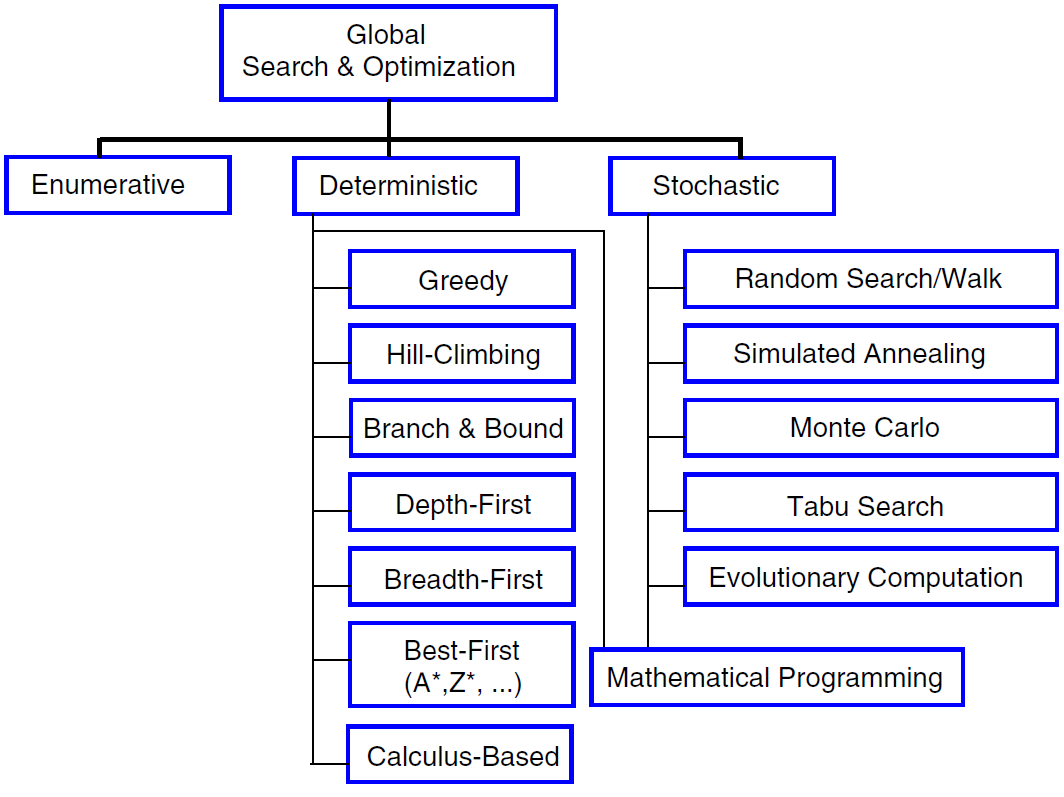
\includegraphics[width=\linewidth]{imagens/classificacao_metodos_busca.png}
	\caption{Técnicas de otimização global - \cite{Coello2007}}
	\label{fig:classificacao_metodos_busca}
\end{figure}

Dentre a categoria dos métodos estocásticos existem os que são completamente aleatórios, como a busca randômica (ou passeio aleatório -- \textit{random walk}), e os que são de alguma forma guiado como o método de resfriamento simulado (\textit{simulated annealling}) por exemplo. O algoritmo evolucionário se encaixa nessa ultima definição, onde existem componentes aleatórios atuando na seleção e reprodução dos indivíduos mas de forma guiada pelos resultados da função de avaliação.

De acordo com \citeauthor{Linden2008}, os Algoritmos Evolucionários são \textbf{heurísticas}\footnote{Heurísticas são algoritmos polinomiais que usualmente tendem a encontrar soluções ótimas ou próximas delas, mas sem garantias} que não asseguram obter o melhor resultado possível, e além disso o resultado pode diferir entre as execuções do algoritmo.

Para \citeauthor{Sivanandam2007}, um algoritmo evolucionário são processos estocásticos e iterativos que operam em um conjunto de indivíduos (população). Cada individuo representa uma possível solução para o problema de otimização ou busca, sendo que os parâmetros estão de alguma forma codificados nesses indivíduos. A população inicial é gerada aleatoriamente e são avaliados usando alguma função, que determina o quão bem o indivíduo responde ao problema. Esse valor determina a direção de busca do algoritmo. 

\section{Biologia}
A ideia por trás dos algoritmos evolucionários e por consequência do algoritmo genético, é a teoria de evolução das espécies na natureza de \textbf{Darwin}, onde a sobrevivência de cada indivíduo é determinada por como ele se adapta ao seu meio. Assim aqueles que conseguiam vantagens sobre os demais por ter uma maior sobrevivência se reproduziam mais, e assim, passavam para as próximas gerações essas características que os diferenciavam. Darwin chamou de seleção natural esse mecanismo da sobrevivência dos mais aptos.

Contudo Darwin não sabia explicar como essa informação era passada dos ancestrais para os descendentes, onde então entram as descobertas de \textbf{Mendel}, que através dos conceitos de genética determinava como características eram compartilhadas entre pais e filhos. 

A unidade básica de informação é o gene, que é um bloco de sequências de DNA e o conjunto de genes formam o cromossomo. Cada gene tem um \textit{locus}, que define a região dentro do cromossomo onde está localizado, e possui um conjunto de valores possíveis chamados de alelos. Os genes controlam as características do indivíduo, sendo que a expressão dessas no individuo é denominada de fenótipo. Assim um conjunto específicos de genes define o genótipo do indivíduo que está associado a um fenótipo, que apresenta as características codificadas no genótipo e que podem ser modificadas pelo ambiente. 

Organismos com cromossomos combinados em pares são chamados de diplóides em contraste com os que não possuem pares, chamados de haplóides. Na natureza a maioria dos seres mais complexos que se reproduzem sexualmente são normalmente diplóides e possuem um ou mais pares de cromossomos sendo que sua quantidade e tamanho dependem de cada ser vivo.

Durante a reprodução, que pode ser de dois tipos, assexuada ou sexuada, ocorre a transmissão da informação. Na reprodução assexuada, o organismo replica a si mesmo, e está mais presente em seres simples. Não apresenta tanta diversidade por não existir combinação de material genético entre dois seres, e fica sujeita apenas a alterações por mutação na cópia.

Na reprodução sexuada de seres diplóides, há presença de dois indivíduos que compartilham seu material genético para formar um novo organismo. No inicio da reprodução, existe a cópia do material genético e recombinação, também chamada de \textit{crossover}(\autoref{fig:crossover_example}). Esse processo é feito com os cromossomos se cruzando um sobre o outro, por isso o termo \textit{crossover}, em um ou mais pontos havendo assim a troca nas sequências de genes. Após feita a recombinação, o material genético é divido em gametas que então são combinados com os gametas do outro pai para formar novamente um cromossomo diplódie completo, gerando assim os novos indivíduos. Para organismos haplóides é feita apenas a combinação das sequencias de cada pai.

\begin{figure}[ht]
	\begin{center}
	\includegraphics[width=0.5\textwidth]{imagens/cross_over.png}
	\caption{Exemplo de reprodução com crossover - \cite{Klug2011}}
	\label{fig:crossover_example}
	\end{center}
\end{figure}


Dentro da etapa de replicação do DNA podem ocorrer erros ou alterações influenciadas por fatores externos, gerando assim as mutações. Isso pode ser positivo, negativo ou não influenciar o resultado final, mas é um outro mecanismo que pode determinar a evolução das espécies.

Os genes definem as características dos indivíduos, mas também existe interação entre os genes, chamada de epistasia (\textit{epistasis}), podendo um par de genes mascarar ou modificar a característica final de outro par de genes. \cite{Klug2011}. Isso é importante do ponto de vista do algoritmo genético pois nem sempre a melhor avaliação estará associada a um único parâmetro, podendo estar associado a uma combinação de parâmetros.

Mendel ainda definiu o conceito de dominância-recessividade em organismos diplóides, assumindo que cada característica é controlada por pares de genes, sendo recebidos um de cada pai. Assim um dos alelos do gene é dominante sobre o outro apresentando a característica final no individuo, e outro alelo será considerado recessivo. Alguns algoritmos genéticos também implementam a lógica para genes dominantes-recessivos.

O processo de seleção acontece então combinando indivíduos que melhor se adaptaram as condições de sobrevivência. Esse seres selecionados devem gerar novos indivíduos que tenha características ainda melhores. O outro caso pode acontecer também e o novo indivíduo ter piores condições de viver, e assim o processo de seleção natural levará esse espécime a extinção favorecendo outros que se sobressaíram na próxima geração.

A evolução então é um processo adaptativo onde através de mutações e recombinação entre os indivíduos, vão surgindo novas gerações que devem apresentar cada vez mais seres que se adaptam cada vez melhor ao ambiente.

\section{Surgimento do algoritmo genético}

Os algoritmos evolucionários vem sendo estudados a um longo tempo, desde da década de 40 que os cientistas se inspiram na natureza para criar os primeiros passos para a inteligência artificial, passando pela década de 50 onde começam os estudos sobre sistemas adaptativos para gerar soluções candidatas para problemas de difícil solução. Na década de 60 Rechenberg desenvolveu as estratégias evolucionárias (\textit{evolutionary strategies}) usando cromossomos compostos de números reais para estudos com aerofólios. Também apareceu a programação evolucionária, usando estruturas de pequenas máquinas de estados para resolver determinadas tarefas, que evolui para programação genética onde pequenos programas passam a ser as soluções candidatas. Existiram outros trabalhos sobre algoritmos evolucionários, programação evolucionária e algoritmos genéticos nas áreas de otimização e aprendizado de máquina, porém foram os trabalhos de Holland nas décadas de 60 e 70 que consolidou os algoritmos genéticos. \cite{Mitchell1996, Linden2008}

Alguns autores como \citeauthor{Mitchell1996}, \citeauthor{LeeJacobson2015}, \citeauthor{Kwong2001} entre outros citam Holland como criador do algoritmo genético(\textit{Genethic Algorithm} ou GA) em 1975 no livro \textit{"Adaptation in Natural and Artificial Systems"}. Nele Holland formaliza uma estrutura para sistemas adaptativos, e enquadra o GA nessa estrutura como uma abstração para a evolução biológica.

O objetivo de Holland não era fazer algo especifico mas sim analisar os sistemas adaptativos e criar uma solução computacional que simulasse os processos encontrados nos sistemas de adaptação natural. Para isso cria uma abstração da evolução na biologia usando uma estrutural formal teórica que poderia atender diversos sistemas evolutivos e não somente o GA. Na formulação do GA por ele, os cromossomos usam representações binárias e os operadores utilizados são o de crossover, inversão e mutação inspirados na genética. O fato de ter usado cromossomos binários serviu de influência para vários outros estudos que se seguiram, mas será exposto no \autoref{chap:GA} que existem outras formas de representar os cromossomos que dependem exclusivamente do problema a ser estudado.

O algoritmo genético geral proposto por Holland se baseia em uma população de cromossomos com alelos `0' e `1' e com os operadores de crossover, mutação e inversão. As evoluções seguiam os seguintes passos: 
\begin{enumerate}
	\item \label{en:loop} Seleção de um cromossomo na população de forma estocástica baseada nas avaliações de todos os cromossomos
	\item \label{en:gene} Aplicações dos operadores genéticos sobre uma cópia do individuo selecionado em \ref{en:loop}.
	\item Seleção de outro cromossomo de forma aleatória com probabilidade igual para todos a ser substituído pelo novo cromossomo gerado em \ref{en:gene}
	\item Avaliar o novo cromossomo
	\item Retornar ao \ref{en:loop}
\end{enumerate}

Essa é uma descrição bem resumida sobre o algoritmo e serve de base para as derivações. Por exemplo no caso do uso de um operador de crossover no \autoref{en:gene}, há a necessidade de seleção de outro cromossomo para formar um par e assim gerar uma nova estrutura.

Avaliando o algoritmo, temos alguns itens básicos que estarão presentes. A codificação do cromossomo para representar os parâmetros das soluções para os problemas. Uma população de cromossomos que serão avaliados simultaneamente durante as iterações do processo. A função de avaliação, que baseada nos parâmetros de cada estrutura irá fornecer uma forma de comparar os diversos elementos presentes na população. Os operadores genéticos que serão usados, sendo que podem ser combinados de diversas formas. 

De acordo com \citeauthor{Mitchell1996} existem três operadores para o algoritmo mais simples:
\begin{description}
	\item[Seleção --] seleciona cromossomos favorecendo os que tem melhor função de avaliação
	\item[Crossover --] também chamado de recombinação, combina dois cromossomos na geração de um novo
	\item[Mutação --] Altera de forma aleatória alguns alelos dos cromossomos, por exemplo em uma codificação binária seria alterar um dos bits do parâmetro.
\end{description}

No \autoref{chap:GA} será explorado com mais detalhes cada um dos operadores. \citeauthor{Holland1992} também descreve um operador de inversão, que apesar de garantir uma melhor diversidade genética impõe uma carga computacional grande para os ganhos efetivos, e nos trabalhos mais recentes se tornou um operador quase nunca usado.

Outro teoria que \citeauthor{Holland1992} formula sobre os GAs é em relação ao processo de paralelismo intrínseco, sobre a forma do algoritmo trabalhar com esquemas (\textit{schemata}) em vez de testar indivíduos específicos da população. \citeauthor{Goldberg1989} aborda esse tema com a hipótese dos blocos de construção (\textit{Building block hypothesis}).

\section {Teorema da inexistência do almoço grátis}
Existe um compromisso entre a eficiência de um algoritmo e sua robustez, isto é, ele pode ser muito eficiente para determinados problemas mas serem ineficientes em outros. Isso implica que não existe um algoritmo que seja eficiente para todos os problemas, e então é razoável supor que algoritmo genético tenha melhor eficiência em determinadas situações. Essa falta de um algoritmo universal é comparado em \cite{Spall2003} a busca de uma agulha no palheiro sem nenhum dado sobre sua posição. Para essa situação a busca aleatória seria um dos melhores métodos de busca e em média nenhum outro seria mais eficiente.

Essa falta de um algoritmo universal para solução dos problemas de otimização parte do teorema da inexistência do almoço grátis (NFL - \textit{No-Free-Lunch Theorem}) proposto por \textbf{Wolpert}. O NFL ainda afirma que todos os algoritmos de busca tem em média o mesmo desempenho \cite{Linden2008}. O que de fato deve ser chamado a atenção é que apesar do apelo do algoritmo comparado com a evolução da espécies, se houver um método específico para determinado problema definitivamente ele será mais eficiente que o GA.

Na \autoref{fig:NFL} \citeauthor{Goldberg1989} mostra que no espectro de problemas de busca e otimização, um método especializado em determinado problema sempre terá a maior eficiência e que os métodos aleatórios e enumerativos apesar de serem considerados menos eficientes podem ter desempenho melhor que o método específico em um espectro mais amplo. O método robusto representa um algoritmo idealizado para solução dos problemas em todas as variedades de problemas. Seria interessante ter um algoritmo robusto, mesmo abandonando o pico de eficiência pois assim atenderia uma variedade de problemas. Como tal algoritmo não é conhecido o que pode ser feito é usar métodos híbridos combinando mais de uma técnica.

\begin{figure}[ht]
	\begin{center}
		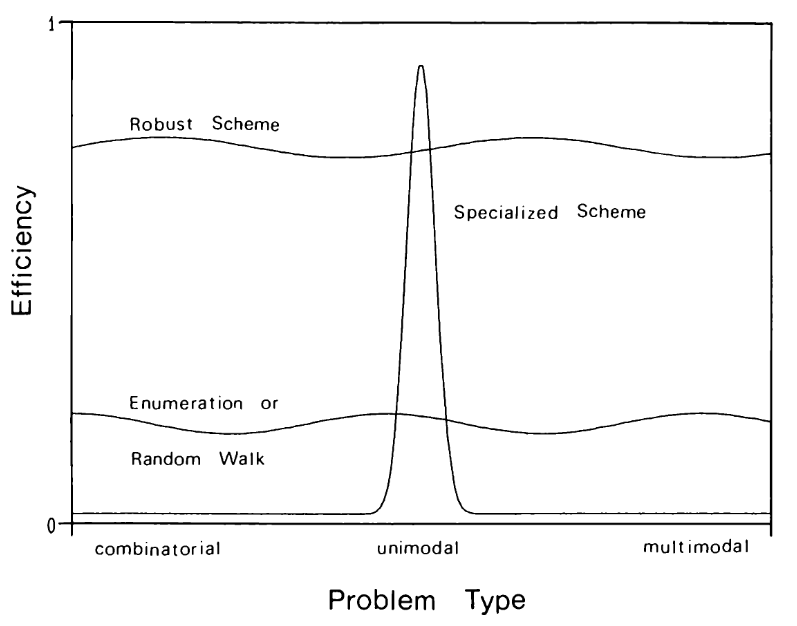
\includegraphics[width=0.5\textwidth]{imagens/David_NFL_Theorem.png}
		\caption{Exemplo para NFL - \cite{Goldberg1989}}
		\label{fig:NFL}
	\end{center}
\end{figure}

% ----------------------------------------------------------

% ----------------------------------------------------------
% PARTE
% ----------------------------------------------------------
%\part{Preparação da pesquisa}
% ----------------------------------------------------------

% ---
% Capitulo com exemplos de comandos inseridos de arquivo externo 
% ---
%%% abtex2-modelo-include-comandos.tex, v-1.9.7 laurocesar
%% Copyright 2012-2018 by abnTeX2 group at http://www.abntex.net.br/ 
%%
%% This work may be distributed and/or modified under the
%% conditions of the LaTeX Project Public License, either version 1.3
%% of this license or (at your option) any later version.
%% The latest version of this license is in
%%   http://www.latex-project.org/lppl.txt
%% and version 1.3 or later is part of all distributions of LaTeX
%% version 2005/12/01 or later.
%%
%% This work has the LPPL maintenance status `maintained'.
%% 
%% The Current Maintainer of this work is the abnTeX2 team, led
%% by Lauro César Araujo. Further information are available on 
%% http://www.abntex.net.br/
%%
%% This work consists of the files abntex2-modelo-include-comandos.tex
%% and abntex2-modelo-img-marca.pdf
%%

% ---
% Este capítulo, utilizado por diferentes exemplos do abnTeX2, ilustra o uso de
% comandos do abnTeX2 e de LaTeX.
% ---
 
\chapter{Resultados de comandos}\label{cap_exemplos}

\chapterprecis{Isto é uma sinopse de capítulo. A ABNT não traz nenhuma
normatização a respeito desse tipo de resumo, que é mais comum em romances 
e livros técnicos.}\index{sinopse de capítulo}

% ---
\section{Codificação dos arquivos: UTF8}
% ---

A codificação de todos os arquivos do \abnTeX\ é \texttt{UTF8}. É necessário que
você utilize a mesma codificação nos documentos que escrever, inclusive nos
arquivos de base bibliográficas |.bib|.

% ---
\section{Citações diretas}
\label{sec-citacao}
% ---

\index{citações!diretas}Utilize o ambiente \texttt{citacao} para incluir
citações diretas com mais de três linhas:

\begin{citacao}
As citações diretas, no texto, com mais de três linhas, devem ser
destacadas com recuo de 4 cm da margem esquerda, com letra menor que a do texto
utilizado e sem as aspas. No caso de documentos datilografados, deve-se
observar apenas o recuo \cite[5.3]{NBR10520:2002}.
\end{citacao}

Use o ambiente assim:

\begin{verbatim}
\begin{citacao}
As citações diretas, no texto, com mais de três linhas [...] deve-se observar
apenas o recuo \cite[5.3]{NBR10520:2002}.
\end{citacao}
\end{verbatim}

O ambiente \texttt{citacao} pode receber como parâmetro opcional um nome de
idioma previamente carregado nas opções da classe (\autoref{sec-hifenizacao}). Nesse
caso, o texto da citação é automaticamente escrito em itálico e a hifenização é
ajustada para o idioma selecionado na opção do ambiente. Por exemplo:

\begin{verbatim}
\begin{citacao}[english]
Text in English language in italic with correct hyphenation.
\end{citacao}
\end{verbatim}

Tem como resultado:

\begin{citacao}[english]
Text in English language in italic with correct hyphenation.
\end{citacao}

\index{citações!simples}Citações simples, com até três linhas, devem ser
incluídas com aspas. Observe que em \LaTeX as aspas iniciais são diferentes das
finais: ``Amor é fogo que arde sem se ver''.

% ---
\section{Notas de rodapé}
% ---

As notas de rodapé são detalhadas pela NBR 14724:2011 na seção 5.2.1\footnote{As
notas devem ser digitadas ou datilografadas dentro das margens, ficando
separadas do texto por um espaço simples de entre as linhas e por filete de 5
cm, a partir da margem esquerda. Devem ser alinhadas, a partir da segunda linha
da mesma nota, abaixo da primeira letra da primeira palavra, de forma a destacar
o expoente, sem espaço entre elas e com fonte menor
\citeonline[5.2.1]{NBR14724:2011}.}\footnote{Caso uma série de notas sejam
criadas sequencialmente, o \abnTeX\ instrui o \LaTeX\ para que uma vírgula seja
colocada após cada número do expoente que indica a nota de rodapé no corpo do
texto.}\footnote{Verifique se os números do expoente possuem uma vírgula para
dividi-los no corpo do texto.}. 


% ---
\section{Tabelas}
% ---

\index{tabelas}A \autoref{tab-nivinv} é um exemplo de tabela construída em
\LaTeX.

\begin{table}[htb]
\ABNTEXfontereduzida
\caption[Níveis de investigação]{Níveis de investigação.}
\label{tab-nivinv}
\begin{tabular}{p{2.6cm}|p{6.0cm}|p{2.25cm}|p{3.40cm}}
  %\hline
   \textbf{Nível de Investigação} & \textbf{Insumos}  & \textbf{Sistemas de Investigação}  & \textbf{Produtos}  \\
    \hline
    Meta-nível & Filosofia\index{filosofia} da Ciência  & Epistemologia &
    Paradigma  \\
    \hline
    Nível do objeto & Paradigmas do metanível e evidências do nível inferior &
    Ciência  & Teorias e modelos \\
    \hline
    Nível inferior & Modelos e métodos do nível do objeto e problemas do nível inferior & Prática & Solução de problemas  \\
   % \hline
\end{tabular}
\legend{Fonte: \citeonline{van86}}
\end{table}

Já a \autoref{tabela-ibge} apresenta uma tabela criada conforme o padrão do
\citeonline{ibge1993} requerido pelas normas da ABNT para documentos técnicos e
acadêmicos.

\begin{table}[htb]
\IBGEtab{%
  \caption{Um Exemplo de tabela alinhada que pode ser longa
  ou curta, conforme padrão IBGE.}%
  \label{tabela-ibge}
}{%
  \begin{tabular}{ccc}
  \toprule
   Nome & Nascimento & Documento \\
  \midrule \midrule
   Maria da Silva & 11/11/1111 & 111.111.111-11 \\
  \midrule 
   João Souza & 11/11/2111 & 211.111.111-11 \\
  \midrule 
   Laura Vicuña & 05/04/1891 & 3111.111.111-11 \\
  \bottomrule
\end{tabular}%
}{%
  \fonte{Produzido pelos autores.}%
  \nota{Esta é uma nota, que diz que os dados são baseados na
  regressão linear.}%
  \nota[Anotações]{Uma anotação adicional, que pode ser seguida de várias
  outras.}%
  }
\end{table}


% ---
\section{Figuras}
% ---

\index{figuras}Figuras podem ser criadas diretamente em \LaTeX,
como o exemplo da \autoref{fig_circulo}.

\begin{figure}[htb]
	\caption{\label{fig_circulo}A delimitação do espaço}
	\begin{center}
	    \setlength{\unitlength}{5cm}
		\begin{picture}(1,1)
		\put(0,0){\line(0,1){1}}
		\put(0,0){\line(1,0){1}}
		\put(0,0){\line(1,1){1}}
		\put(0,0){\line(1,2){.5}}
		\put(0,0){\line(1,3){.3333}}
		\put(0,0){\line(1,4){.25}}
		\put(0,0){\line(1,5){.2}}
		\put(0,0){\line(1,6){.1667}}
		\put(0,0){\line(2,1){1}}
		\put(0,0){\line(2,3){.6667}}
		\put(0,0){\line(2,5){.4}}
		\put(0,0){\line(3,1){1}}
		\put(0,0){\line(3,2){1}}
		\put(0,0){\line(3,4){.75}}
		\put(0,0){\line(3,5){.6}}
		\put(0,0){\line(4,1){1}}
		\put(0,0){\line(4,3){1}}
		\put(0,0){\line(4,5){.8}}
		\put(0,0){\line(5,1){1}}
		\put(0,0){\line(5,2){1}}
		\put(0,0){\line(5,3){1}}
		\put(0,0){\line(5,4){1}}
		\put(0,0){\line(5,6){.8333}}
		\put(0,0){\line(6,1){1}}
		\put(0,0){\line(6,5){1}}
		\end{picture}
	\end{center}
	\legend{Fonte: os autores}
\end{figure}

Ou então figuras podem ser incorporadas de arquivos externos, como é o caso da
\autoref{fig_grafico}. Se a figura que for incluída se tratar de um diagrama, um
gráfico ou uma ilustração que você mesmo produza, priorize o uso de imagens
vetoriais no formato PDF. Com isso, o tamanho do arquivo final do trabalho será
menor, e as imagens terão uma apresentação melhor, principalmente quando
impressas, uma vez que imagens vetorias são perfeitamente escaláveis para
qualquer dimensão. Nesse caso, se for utilizar o Microsoft Excel para produzir
gráficos, ou o Microsoft Word para produzir ilustrações, exporte-os como PDF e
os incorpore ao documento conforme o exemplo abaixo. No entanto, para manter a
coerência no uso de software livre (já que você está usando \LaTeX e \abnTeX),
teste a ferramenta \textsf{InkScape}\index{InkScape}
(\url{http://inkscape.org/}). Ela é uma excelente opção de código-livre para
produzir ilustrações vetoriais, similar ao CorelDraw\index{CorelDraw} ou ao Adobe
Illustrator\index{Adobe Illustrator}. De todo modo, caso não seja possível
utilizar arquivos de imagens como PDF, utilize qualquer outro formato, como
JPEG, GIF, BMP, etc. Nesse caso, você pode tentar aprimorar as imagens
incorporadas com o software livre \textsf{Gimp}\index{Gimp}
(\url{http://www.gimp.org/}). Ele é uma alternativa livre ao Adobe
Photoshop\index{Adobe Photoshop}.

\begin{figure}[htb]
	\caption{\label{fig_grafico}Gráfico produzido em Excel e salvo como PDF}
	\begin{center}
	    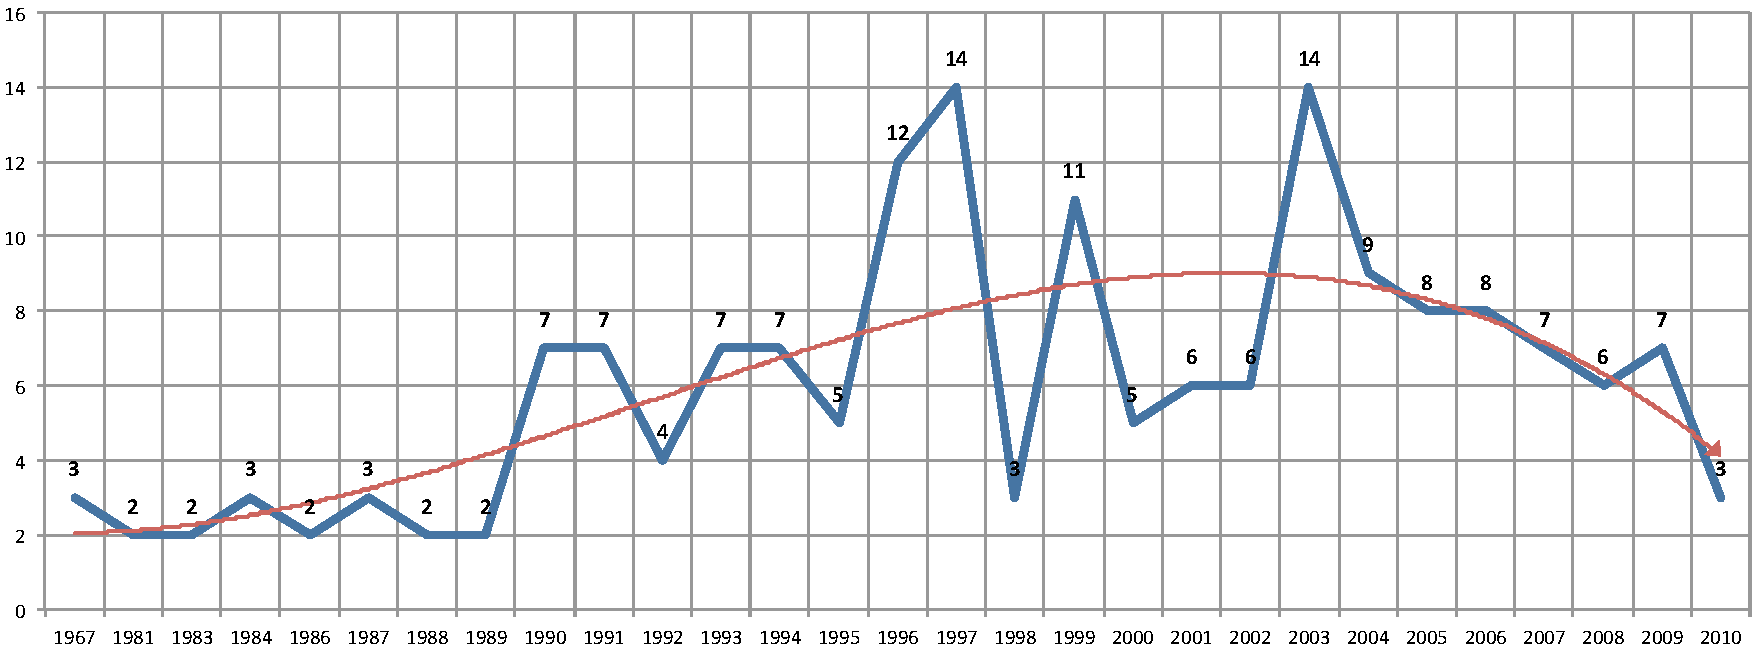
\includegraphics[scale=0.5]{abntex2-modelo-img-grafico.pdf}
	\end{center}
	\legend{Fonte: \citeonline[p. 24]{araujo2012}}
\end{figure}

% ---
\subsection{Figuras em \emph{minipages}}
% ---

\emph{Minipages} são usadas para inserir textos ou outros elementos em quadros
com tamanhos e posições controladas. Veja o exemplo da
\autoref{fig_minipage_imagem1} e da \autoref{fig_minipage_grafico2}.

\begin{figure}[htb]
 \label{teste}
 \centering
  \begin{minipage}{0.4\textwidth}
    \centering
    \caption{Imagem 1 da minipage} \label{fig_minipage_imagem1}
    
\includegraphics[scale=0.9]{abntex2-modelo-img-marca.pdf}
    \legend{Fonte: Produzido pelos autores}
  \end{minipage}
  \hfill
  \begin{minipage}{0.4\textwidth}
    \centering
    \caption{Grafico 2 da minipage} \label{fig_minipage_grafico2}
    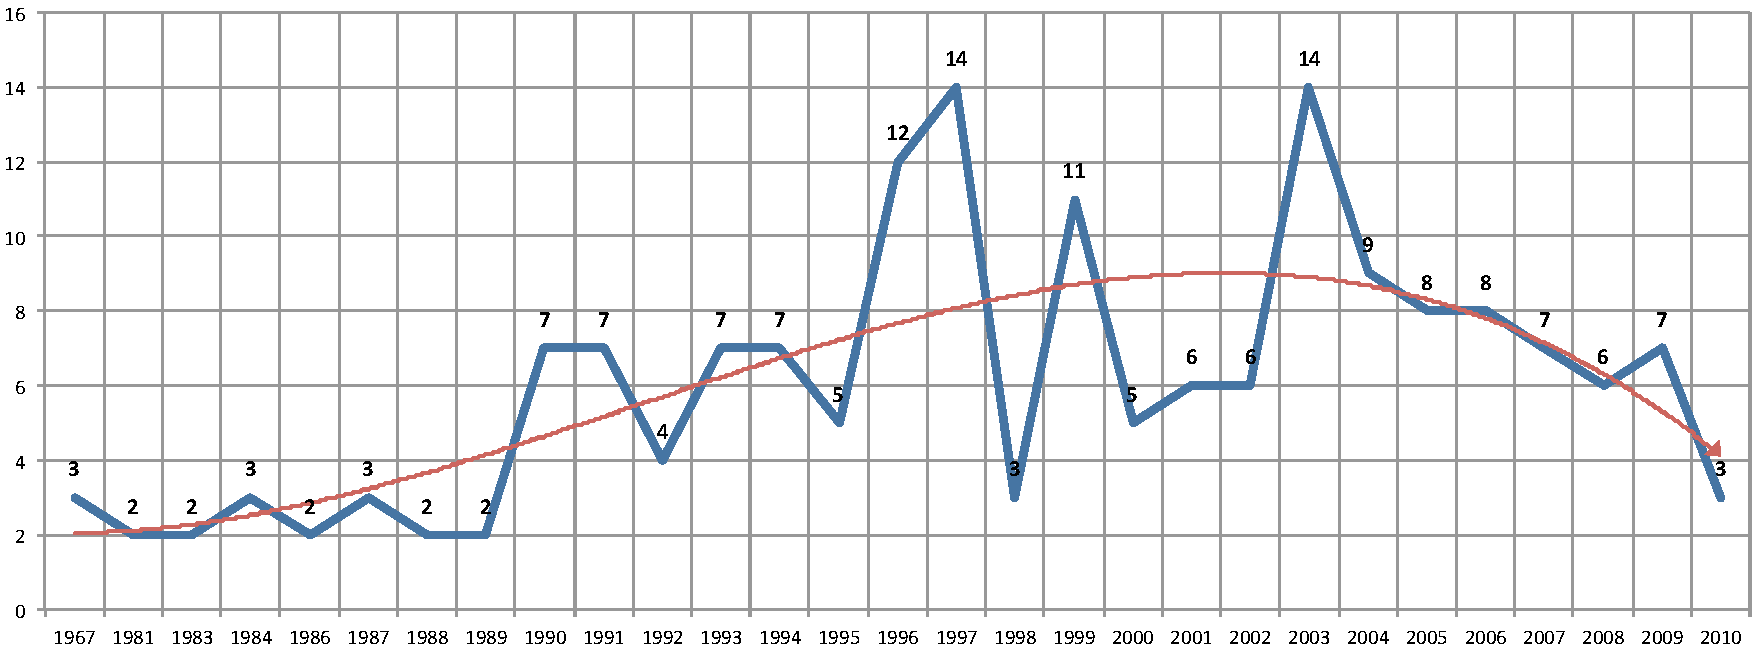
\includegraphics[scale=0.2]{abntex2-modelo-img-grafico.pdf}
    \legend{Fonte: \citeonline[p. 24]{araujo2012}}
  \end{minipage}
\end{figure}

Observe que, segundo a \citeonline[seções 4.2.1.10 e 5.8]{NBR14724:2011}, as
ilustrações devem sempre ter numeração contínua e única em todo o documento:

\begin{citacao}
Qualquer que seja o tipo de ilustração, sua identificação aparece na parte
superior, precedida da palavra designativa (desenho, esquema, fluxograma,
fotografia, gráfico, mapa, organograma, planta, quadro, retrato, figura,
imagem, entre outros), seguida de seu número de ordem de ocorrência no texto,
em algarismos arábicos, travessão e do respectivo título. Após a ilustração, na
parte inferior, indicar a fonte consultada (elemento obrigatório, mesmo que
seja produção do próprio autor), legenda, notas e outras informações
necessárias à sua compreensão (se houver). A ilustração deve ser citada no
texto e inserida o mais próximo possível do trecho a que se
refere. \cite[seções 5.8]{NBR14724:2011}
\end{citacao}

% ---
\section{Expressões matemáticas}
% ---

\index{expressões matemáticas}Use o ambiente \texttt{equation} para escrever
expressões matemáticas numeradas:

\begin{equation}
  \forall x \in X, \quad \exists \: y \leq \epsilon
\end{equation}

Escreva expressões matemáticas entre \$ e \$, como em $ \lim_{x \to \infty}
\exp(-x) = 0 $, para que fiquem na mesma linha.

Também é possível usar colchetes para indicar o início de uma expressão
matemática que não é numerada.

\[
\left|\sum_{i=1}^n a_ib_i\right|
\le
\left(\sum_{i=1}^n a_i^2\right)^{1/2}
\left(\sum_{i=1}^n b_i^2\right)^{1/2}
\]

Consulte mais informações sobre expressões matemáticas em
\url{https://github.com/abntex/abntex2/wiki/Referencias}.

% ---
\section{Enumerações: alíneas e subalíneas}
% ---

\index{alíneas}\index{subalíneas}\index{incisos}Quando for necessário enumerar
os diversos assuntos de uma seção que não possua título, esta deve ser
subdividida em alíneas \cite[4.2]{NBR6024:2012}:

\begin{alineas}

  \item os diversos assuntos que não possuam título próprio, dentro de uma mesma
  seção, devem ser subdivididos em alíneas; 
  
  \item o texto que antecede as alíneas termina em dois pontos;
  \item as alíneas devem ser indicadas alfabeticamente, em letra minúscula,
  seguida de parêntese. Utilizam-se letras dobradas, quando esgotadas as
  letras do alfabeto;

  \item as letras indicativas das alíneas devem apresentar recuo em relação à
  margem esquerda;

  \item o texto da alínea deve começar por letra minúscula e terminar em
  ponto-e-vírgula, exceto a última alínea que termina em ponto final;

  \item o texto da alínea deve terminar em dois pontos, se houver subalínea;

  \item a segunda e as seguintes linhas do texto da alínea começa sob a
  primeira letra do texto da própria alínea;
  
  \item subalíneas \cite[4.3]{NBR6024:2012} devem ser conforme as alíneas a
  seguir:

  \begin{alineas}
     \item as subalíneas devem começar por travessão seguido de espaço;

     \item as subalíneas devem apresentar recuo em relação à alínea;

     \item o texto da subalínea deve começar por letra minúscula e terminar em
     ponto-e-vírgula. A última subalínea deve terminar em ponto final, se não
     houver alínea subsequente;

     \item a segunda e as seguintes linhas do texto da subalínea começam sob a
     primeira letra do texto da própria subalínea.
  \end{alineas}
  
  \item no \abnTeX\ estão disponíveis os ambientes \texttt{incisos} e
  \texttt{subalineas}, que em suma são o mesmo que se criar outro nível de
  \texttt{alineas}, como nos exemplos à seguir:
  
  \begin{incisos}
    \item \textit{Um novo inciso em itálico};
  \end{incisos}
  
  \item Alínea em \textbf{negrito}:
  
  \begin{subalineas}
    \item \textit{Uma subalínea em itálico};
    \item \underline{\textit{Uma subalínea em itálico e sublinhado}}; 
  \end{subalineas}
  
  \item Última alínea com \emph{ênfase}.
  
\end{alineas}

% ---
\section{Espaçamento entre parágrafos e linhas}
% ---

\index{espaçamento!dos parágrafos}O tamanho do parágrafo, espaço entre a margem
e o início da frase do parágrafo, é definido por:

\begin{verbatim}
   \setlength{\parindent}{1.3cm}
\end{verbatim}

\index{espaçamento!do primeiro parágrafo}Por padrão, não há espaçamento no
primeiro parágrafo de cada início de divisão do documento
(\autoref{sec-divisoes}). Porém, você pode definir que o primeiro parágrafo
também seja indentado, como é o caso deste documento. Para isso, apenas inclua o
pacote \textsf{indentfirst} no preâmbulo do documento:

\begin{verbatim}
   \usepackage{indentfirst}      % Indenta o primeiro parágrafo de cada seção.
\end{verbatim}

\index{espaçamento!entre os parágrafos}O espaçamento entre um parágrafo e outro
pode ser controlado por meio do comando:

\begin{verbatim}
  \setlength{\parskip}{0.2cm}  % tente também \onelineskip
\end{verbatim}

\index{espaçamento!entre as linhas}O controle do espaçamento entre linhas é
definido por:

\begin{verbatim}
  \OnehalfSpacing       % espaçamento um e meio (padrão); 
  \DoubleSpacing        % espaçamento duplo
  \SingleSpacing        % espaçamento simples	
\end{verbatim}

Para isso, também estão disponíveis os ambientes:

\begin{verbatim}
  \begin{SingleSpace} ...\end{SingleSpace}
  \begin{Spacing}{hfactori} ... \end{Spacing}
  \begin{OnehalfSpace} ... \end{OnehalfSpace}
  \begin{OnehalfSpace*} ... \end{OnehalfSpace*}
  \begin{DoubleSpace} ... \end{DoubleSpace}
  \begin{DoubleSpace*} ... \end{DoubleSpace*} 
\end{verbatim}

Para mais informações, consulte \citeonline[p. 47-52 e 135]{memoir}.

% ---
\section{Inclusão de outros arquivos}\label{sec-include}
% ---

É uma boa prática dividir o seu documento em diversos arquivos, e não
apenas escrever tudo em um único. Esse recurso foi utilizado neste
documento. Para incluir diferentes arquivos em um arquivo principal,
de modo que cada arquivo incluído fique em uma página diferente, utilize o
comando:

\begin{verbatim}
   \include{documento-a-ser-incluido}      % sem a extensão .tex
\end{verbatim}

Para incluir documentos sem quebra de páginas, utilize:

\begin{verbatim}
   \input{documento-a-ser-incluido}      % sem a extensão .tex
\end{verbatim}

% ---
\section{Compilar o documento \LaTeX}
% ---

Geralmente os editores \LaTeX, como o
TeXlipse\footnote{\url{http://texlipse.sourceforge.net/}}, o
Texmaker\footnote{\url{http://www.xm1math.net/texmaker/}}, entre outros,
compilam os documentos automaticamente, de modo que você não precisa se
preocupar com isso.

No entanto, você pode compilar os documentos \LaTeX usando os seguintes
comandos, que devem ser digitados no \emph{Prompt de Comandos} do Windows ou no
\emph{Terminal} do Mac ou do Linux:

\begin{verbatim}
   pdflatex ARQUIVO_PRINCIPAL.tex
   bibtex ARQUIVO_PRINCIPAL.aux
   makeindex ARQUIVO_PRINCIPAL.idx 
   makeindex ARQUIVO_PRINCIPAL.nlo -s nomencl.ist -o ARQUIVO_PRINCIPAL.nls
   pdflatex ARQUIVO_PRINCIPAL.tex
   pdflatex ARQUIVO_PRINCIPAL.tex
\end{verbatim}

% ---
\section{Remissões internas}
% ---

Ao nomear a \autoref{tab-nivinv} e a \autoref{fig_circulo}, apresentamos um
exemplo de remissão interna, que também pode ser feita quando indicamos o
\autoref{cap_exemplos}, que tem o nome \emph{\nameref{cap_exemplos}}. O número
do capítulo indicado é \ref{cap_exemplos}, que se inicia à
\autopageref{cap_exemplos}\footnote{O número da página de uma remissão pode ser
obtida também assim:
\pageref{cap_exemplos}.}.
Veja a \autoref{sec-divisoes} para outros exemplos de remissões internas entre
seções, subseções e subsubseções.

O código usado para produzir o texto desta seção é:

\begin{verbatim}
Ao nomear a \autoref{tab-nivinv} e a \autoref{fig_circulo}, apresentamos um
exemplo de remissão interna, que também pode ser feita quando indicamos o
\autoref{cap_exemplos}, que tem o nome \emph{\nameref{cap_exemplos}}. O número
do capítulo indicado é \ref{cap_exemplos}, que se inicia à
\autopageref{cap_exemplos}\footnote{O número da página de uma remissão pode ser
obtida também assim:
\pageref{cap_exemplos}.}.
Veja a \autoref{sec-divisoes} para outros exemplos de remissões internas entre
seções, subseções e subsubseções.
\end{verbatim}

% ---
\section{Divisões do documento: seção}\label{sec-divisoes}
% ---

Esta seção testa o uso de divisões de documentos. Esta é a
\autoref{sec-divisoes}. Veja a \autoref{sec-divisoes-subsection}.

\subsection{Divisões do documento: subseção}\label{sec-divisoes-subsection}

Isto é uma subseção. Veja a \autoref{sec-divisoes-subsubsection}, que é uma
\texttt{subsubsection} do \LaTeX, mas é impressa chamada de ``subseção'' porque
no Português não temos a palavra ``subsubseção''.

\subsubsection{Divisões do documento: subsubseção}
\label{sec-divisoes-subsubsection}

Isto é uma subsubseção.

\subsubsection{Divisões do documento: subsubseção}

Isto é outra subsubseção.

\subsection{Divisões do documento: subseção}\label{sec-exemplo-subsec}

Isto é uma subseção.

\subsubsection{Divisões do documento: subsubseção}

Isto é mais uma subsubseção da \autoref{sec-exemplo-subsec}.


\subsubsubsection{Esta é uma subseção de quinto
nível}\label{sec-exemplo-subsubsubsection}

Esta é uma seção de quinto nível. Ela é produzida com o seguinte comando:

\begin{verbatim}
\subsubsubsection{Esta é uma subseção de quinto
nível}\label{sec-exemplo-subsubsubsection}
\end{verbatim}

\subsubsubsection{Esta é outra subseção de quinto nível}\label{sec-exemplo-subsubsubsection-outro}

Esta é outra seção de quinto nível.


\paragraph{Este é um parágrafo numerado}\label{sec-exemplo-paragrafo}

Este é um exemplo de parágrafo nomeado. Ele é produzida com o comando de
parágrafo:

\begin{verbatim}
\paragraph{Este é um parágrafo nomeado}\label{sec-exemplo-paragrafo}
\end{verbatim}

A numeração entre parágrafos numeradaos e subsubsubseções são contínuas.

\paragraph{Esta é outro parágrafo numerado}\label{sec-exemplo-paragrafo-outro}

Esta é outro parágrafo nomeado.

% ---
\section{Este é um exemplo de nome de seção longo. Ele deve estar
alinhado à esquerda e a segunda e demais linhas devem iniciar logo abaixo da
primeira palavra da primeira linha}
% ---

Isso atende à norma \citeonline[seções de 5.2.2 a 5.2.4]{NBR14724:2011} 
 e \citeonline[seções de 3.1 a 3.8]{NBR6024:2012}.

% ---
\section{Diferentes idiomas e hifenizações}
\label{sec-hifenizacao}
% ---

Para usar hifenizações de diferentes idiomas, inclua nas opções do documento o
nome dos idiomas que o seu texto contém. Por exemplo (para melhor
visualização, as opções foram quebras em diferentes linhas):

\begin{verbatim}
\documentclass[
	12pt,
	openright,
	twoside,
	a4paper,
	english,
	french,
	spanish,
	brazil
	]{abntex2}
\end{verbatim}

O idioma português-brasileiro (\texttt{brazil}) é incluído automaticamente pela
classe \textsf{abntex2}. Porém, mesmo assim a opção \texttt{brazil} deve ser
informada como a última opção da classe para que todos os pacotes reconheçam o
idioma. Vale ressaltar que a última opção de idioma é a utilizada por padrão no
documento. Desse modo, caso deseje escrever um texto em inglês que tenha
citações em português e em francês, você deveria usar o preâmbulo como abaixo:

\begin{verbatim}
\documentclass[
	12pt,
	openright,
	twoside,
	a4paper,
	french,
	brazil,
	english
	]{abntex2}
\end{verbatim}

A lista completa de idiomas suportados, bem como outras opções de hifenização,
estão disponíveis em \citeonline[p.~5-6]{babel}.

Exemplo de hifenização em inglês\footnote{Extraído de:
\url{http://en.wikibooks.org/wiki/LaTeX/Internationalization}}:

\begin{otherlanguage*}{english}
\textit{Text in English language. This environment switches all language-related
definitions, like the language specific names for figures, tables etc. to the other
language. The starred version of this environment typesets the main text
according to the rules of the other language, but keeps the language specific
string for ancillary things like figures, in the main language of the document.
The environment hyphenrules switches only the hyphenation patterns used; it can
also be used to disallow hyphenation by using the language name
`nohyphenation'.}
\end{otherlanguage*}

Exemplo de hifenização em francês\footnote{Extraído de:
\url{http://bigbrowser.blog.lemonde.fr/2013/02/17/tu-ne-tweeteras-point-le-vatican-interdit-aux-cardinaux-de-tweeter-pendant-le-conclave/}}:

\begin{otherlanguage*}{french}
\textit{Texte en français. Pas question que Twitter ne vienne faire une
concurrence déloyale à la traditionnelle fumée blanche qui marque l'élection
d'un nouveau pape. Pour éviter toute fuite précoce, le Vatican a donc pris un
peu d'avance, et a déjà interdit aux cardinaux qui prendront part au vote
d'utiliser le réseau social, selon Catholic News Service. Une mesure valable
surtout pour les neuf cardinaux – sur les 117 du conclave – pratiquants très
actifs de Twitter, qui auront interdiction pendant toute la période de se
connecter à leur compte.}
\end{otherlanguage*}

Pequeno texto em espanhol\footnote{Extraído de:
\url{http://internacional.elpais.com/internacional/2013/02/17/actualidad/1361102009_913423.html}}:

\foreignlanguage{spanish}{\textit{Decenas de miles de personas ovacionan al pontífice en su
penúltimo ángelus dominical, el primero desde que anunciase su renuncia. El Papa se
centra en la crítica al materialismo}}.

O idioma geral do texto por ser alterado como no exemplo seguinte:

\begin{verbatim}
  \selectlanguage{english}
\end{verbatim}

Isso altera automaticamente a hifenização e todos os nomes constantes de
referências do documento para o idioma inglês. Consulte o manual da classe
\cite{abntex2classe} para obter orientações adicionais sobre internacionalização de
documentos produzidos com \abnTeX.

A \autoref{sec-citacao} descreve o ambiente \texttt{citacao} que pode receber
como parâmetro um idioma a ser usado na citação.

% ---
\section{Consulte o manual da classe \textsf{abntex2}}
% ---

Consulte o manual da classe \textsf{abntex2} \cite{abntex2classe} para uma
referência completa das macros e ambientes disponíveis. 

Além disso, o manual possui informações adicionais sobre as normas ABNT
observadas pelo \abnTeX\ e considerações sobre eventuais requisitos específicos
não atendidos, como o caso da \citeonline[seção 5.2.2]{NBR14724:2011}, que
especifica o espaçamento entre os capítulos e o início do texto, regra
propositalmente não atendida pelo presente modelo.

% ---
\section{Referências bibliográficas}
% ---

A formatação das referências bibliográficas conforme as regras da ABNT são um
dos principais objetivos do \abnTeX. Consulte os manuais
\citeonline{abntex2cite} e \citeonline{abntex2cite-alf} para obter informações
sobre como utilizar as referências bibliográficas.

%-
\subsection{Acentuação de referências bibliográficas}
%-

Normalmente não há problemas em usar caracteres acentuados em arquivos
bibliográficos (\texttt{*.bib}). Porém, como as regras da ABNT fazem uso quase
abusivo da conversão para letras maiúsculas, é preciso observar o modo como se
escreve os nomes dos autores. Na ~\autoref{tabela-acentos} você encontra alguns
exemplos das conversões mais importantes. Preste atenção especial para `ç' e `í'
que devem estar envoltos em chaves. A regra geral é sempre usar a acentuação
neste modo quando houver conversão para letras maiúsculas.

\begin{table}[htbp]
\caption{Tabela de conversão de acentuação.}
\label{tabela-acentos}

\begin{center}
\begin{tabular}{ll}\hline\hline
acento & \textsf{bibtex}\\
à á ã & \verb+\`a+ \verb+\'a+ \verb+\~a+\\
í & \verb+{\'\i}+\\
ç & \verb+{\c c}+\\
\hline\hline
\end{tabular}
\end{center}
\end{table}


% ---
\section{Precisa de ajuda?}
% ---

Consulte a FAQ com perguntas frequentes e comuns no portal do \abnTeX:
\url{https://github.com/abntex/abntex2/wiki/FAQ}.

Inscreva-se no grupo de usuários \LaTeX:
\url{http://groups.google.com/group/latex-br}, tire suas dúvidas e ajude
outros usuários.

Participe também do grupo de desenvolvedores do \abnTeX:
\url{http://groups.google.com/group/abntex2} e faça sua contribuição à
ferramenta.

% ---
\section{Você pode ajudar?}
% ---

Sua contribuição é muito importante! Você pode ajudar na divulgação, no
desenvolvimento e de várias outras formas. Veja como contribuir com o \abnTeX\
em \url{https://github.com/abntex/abntex2/wiki/Como-Contribuir}.

% ---
\section{Quer customizar os modelos do \abnTeX\ para sua instituição ou
universidade?}
% ---

Veja como customizar o \abnTeX\ em:
\url{https://github.com/abntex/abntex2/wiki/ComoCustomizar}.


% ---

% ---
% Capitulo explicando teoria sobre o algoritmo genético
% ---
% ---
% Este capítulo, apresenta os conceitos sobre o algoritmo genético
% ---

\chapter{Algoritmos Genéticos}
\label{chap:GA}

O algoritmo genético (GA) parte de uma população de \textit{cromossomos} que representam as soluções candidatas para o problema de otimização. Cada uma das soluções é avaliada de acordo com critérios inerentes do problema, para posteriormente serem selecionados e combinados de forma a criar novas soluções candidatas.

Já é possível perceber uma das vantagens do algoritmo, ao fazer uma avaliação direta das soluções de forma paralela. Por exemplo em problemas NP-Completos onde são difíceis de se obter soluções numéricas eficientes, mas é possível testar soluções em tempo polinomial, o algoritmo se torna atrativo. O teste de múltiplas soluções facilita o processamento paralelo aumentando a eficiência do algoritmo.

O algoritmo genético mais simples deverá conter pelo menos uma forma de avaliar os elementos da população, uma forma de seleção baseada nas avaliações e operadores genéticos para gerar a nova população.

\citeauthor{Linden2008} afirma que quanto mais conhecimento especifico sobre o problema for incorporado ao GA, melhor eficiência ele terá. Assim ao definir os operadores que serão utilizados é importante ter em mente que eles devem ser adequados ao problema e não ao contrário.

\section{Codificação dos genes}
Cada cromossomo da população possui uma sequência de genes, que representam os parâmetros para solução do problema. Cada gene terá um possível conjunto de valores, os alelos no equivalente biológico, que para o GA será um alfabeto de valores \( \mathcal{A}\), ou um intervalo caso trabalhando com genes de valores reais. O alfabeto mais simples é o binário com \(\mathcal{A} = \{0, 1\}\), e é muito utilizado pela simplicidade e por ter sido originalmente a escolha de \citeauthor{Holland1992} para explicar os esquemas, além disso para ele cromossomos de maior comprimento e com menos alelos geravam mais paralelismo intrínseco. Porém essa questão dos esquemas e paralelismo vem levantado questionamentos sobre sua real contribuição para o algoritmo. 

Com o alfabeto binário, os parâmetros são codificados usando sequências binárias, que podem ser representadas por \textit{strings}. Isso envolve conversões dos parâmetros para binário e vice versa. Os operadores de crossover e mutação ficam simplificados ao utilizar esse tipo de codificação. Uma variação da codificação binária é usar o código gray, que evita o chamado abismo de Hamming\footnote{O abismo de Hamming é o efeito que para mudar o valor inteiro em uma unidade na representação binária é necessário alterar todos os bits, por exemplo para ir do número 7 (0111) para o 8 (1000)} 

A representação dos genes em termos gerais deve ser o mais simples e o mais natural possível ao problema. Então é comum usar outras formas de representar os genes, por exemplo, em um problema de escolha da melhor rota é interessante representar os grafos no cromossomo, com isso uma sequência de números inteiros representando cada vértice seria o mais apropriado. Também tem sido muito utilizada a codificação dos genes como números reais, representando assim diretamente os parâmetros do problema, e adaptando então as técnicas de mutação e crossover para se adequar a essa nova codificação. A representação com números reais é muito presente em problemas de otimização para redes neurais, onde o cromossomo é o conjunto de parâmetros de ajuste da rede.

Quando possível é interessante impor na codificação as restrições que são impostas ao conjunto de soluções. Por exemplo, ao utilizar um alfabeto binário para representar valores inteiros, ou reais, pode ser feita a conversão de maneira que os valores máximos e mínimos da representação binária coincidam com os valores permitidos dos parâmetros após a decodificação dos genes. Com isso mais conhecimento é sobre o problema é agregado ao algoritmo melhorando sua resposta. Nem sempre esses limites serão possíveis e será vista outra maneira de impor as condições ao algoritmo através da avaliação.

\section{População, Avaliação e Seleção}
\label{sec:avaliacao}
\subsection{População}
O conjunto de soluções candidatas é definido como a população do algoritmo, que será modificada a cada iteração através dos operadores genéticos. A cada uma dessas populações geradas no instante \(t\) será dado o nome de geração. O tamanho da população é um parâmetro para o algoritmo, e quanto maior, mais soluções serão testadas em paralelo, porém mais recursos computacionais serão usados para cada geração. No algoritmo mais simples, a população é de tamanho fixo e toda substituída na próxima geração, e em outras formas do algoritmo ela pode ter o tamanho variável.

Não existe um número idealizado para o tamanho da população sendo que boa parte dos trabalhos usam 100 como um parâmetro inicial. \citeauthor{Linden2008} indica que um bom começo seria usar \(40 * p\) onde \(p\) é a quantidade de parâmetros codificados em nosso cromossomo, porém para codificações de grafos ou ordenamentos já não seria prático usar esse tipo de escolha para o tamanho da população.

É importante também definir dois conceitos presentes na literatura sobre os GA, que são o \textit{exploitation}\footnote{Exploitation consiste em testar uma região limitada mas promissora do espaço de soluções com a expectativa de melhorar uma solução já conhecida dentro dessa região} e o \textit{exploration}\footnote{Exploration consiste em testar uma região muito mais ampla do espaço de soluções, com a expectativa de encontrar novas soluções promissoras}. O \textit{exploitation} (aproveitamento) é o fato de explorar cada um dos indivíduos da população pelos potenciais resultados que podem gerar através dos descendentes. Já \textit{exploration} (exploração) é o conceito de se manter a diversidade genética da população de forma a explorar o espaço de soluções de forma completa. \citeauthor{Holland1992} indica que deve existir um equilíbrio entre os dois conceitos na população, pois deve-se aproveitar ao máximo cada solução encontrada que poderá gerar novas soluções melhores, e da mesma maneira manter os horizontes sobre o espaço de soluções aberto para a descoberta de novas soluções, evitando a convergência genética.

Defini-se convergência genética como sendo o fato dos cromossomos presentes na população começarem a ficar todos com a codificação similares, levando a entender que o algoritmo atingiu o objetivo, ou pelo menos um máximo ou minimo local. Algumas GAs criam operadores de comparação entre os cromossomos de forma a quantificar essa proximidade como parâmetro para encerramento do algoritmo, mas o mais comum é executar o processo de iteração por \(T\) gerações. A dificuldade de usar a comparação entre os cromossomos está no custo computacional, que dependendo da forma de codificação usada pode ficar muito complexo. \citeauthor{Linden2008} menciona que uma forma de verificar essa convergência é usando o algoritmo de agrupamento K-Means e e depois comparar a distância entre os centróides gerados pelo algoritmo.

Sobre a população podem existir pequenas variações sobre como é evoluída durante o algoritmo. Uma dessas alterações é o \textbf{elitismo}, que separa os \textit{k} melhores indivíduos para sobreviverem na próxima geração. Isso é usado devido ao fato de que os operadores de crossover e mutação poderem destruir esses indivíduos na geração da próxima geração, perdendo assim os bons resultados alcançados. Essa mudança melhora o equilíbrio entre os conceitos de \textit{exploitation} e \textit{exploration} e consequentemente o desempenho do algoritmo, pois mantemos o \textit{exploitation} sobre os \textit{k} indivíduos preservados entre as gerações, e mantemos o \textit{exploration} dando liberdade de escolha arbitrária para os demais \(n-k\) indivíduos da população, onde normalmente \(n \gg k\). 

Outra estratégia para as populações é chamada de \(\mu + \lambda\), onde são criados \(\lambda\) cromossomos gerados por \(\mu\) indivíduos da população atual (geralmente \(\mu < \lambda\)). Feito isso os \(\mu + \lambda\) cromossomos pais e filhos competem para serem selecionados apenas os \(\mu\) melhores indivíduos para formar a nova população. Essa técnica também pode acelerar a convergência genética, devido ao fato da seleção de apenas os melhores que podem apresentar pouca variação genética, e que para ser compensado deveria ser empregado alguma técnica para manter a diversidade.

Outra alteração possível é denominada \textit{Steady state}, onde em vez de haver a substituição de todos os \textit{n} indivíduos da população anterior para a nova (ou dos \(n - k\) no caso do elitismo) vão sendo criados poucos indivíduos a cada iteração substituindo de forma aleatória os piores pais, isto é, seleciona-se com mais probabilidade os pais com pior avaliação para serem substituídos. Dessa forma existirá uma interação entre cromossomos da geração \textit{t} com as da geração \(t+1\). Um porém de usar essa modificação é de acelerar a convergência genética, pois os indivíduos com pior avaliação sempre serão substituídos de forma rápida, mesmo os recém criados, e também o fato de um cromossomo poder reproduzir com o cromossomo que o gerou, deverá gerar um cromossomo muito parecido com os dois, limitando o \textit{exploitation} desses indivíduos.

Para populações com tamanha variável, basicamente duas técnicas podem ser empregadas, uma para considerar um tempo de vida para cada indivíduo levando em conta su avaliação sobre a média da população, e a outra considerando a variabilidade genética. O método que considera a idade dos indivíduos, mantém eles na população por quanto tempo foi determinado na avaliação, e podem levar a condições que a população cresça indefinidamente ou que seja extinta, sendo necessário um controle extra sobre o tamanho da população.

A técnica levando em conta a diversidade, aumenta a população caso perceba-se, através de algum tipo de medição, que os cromossomos da população são semelhantes. Nesse caso alguns cromossomos gerados aleatoriamente podem ser acrescentados a população de modo a manter a exploração do espaço de soluções. Porém como todas as técnicas que devem comparar semelhança entre cromossomos pode ser custosas computacionalmente.

A população inicial geralmente é iniciada criando cromossomos de forma aleatória, porém pode ser feito de forma a subdividir o espaço de soluções em \textit{n} partes, sendo \textit{n} o tamanho da população, e gerando um cromossomo aleatório para cada uma dessas partes. \cite{Linden2008}.

\subsection{Avaliação}
Para executar uma seleção sobre os cromossomos da população é necessário primeiro existir uma função de avaliação, que deverá fornecer um escalar, de forma a atribuir para cada cromossomo presente na população uma espécie de nota para sua adaptação. O comum nos algoritmos é usar funções de avaliação que são sempre positivas, para o uso no método de seleção da roleta viciada. Alguns cuidados devem ser tomados ao definir a função de avaliação, pois se ela não apresentar variações suficientes para separar os cromossomos que melhor se adaptam dos demais, o algoritmo irá convergir mais lentamente, e se o contrário ocorrer e a função de avaliação tiver valores muito elevados, teremos uma convergência genética rápida demais impedindo a exploração do espaço de soluções podendo ficar restrito a um máximo local.

De uma forma geral consideremos uma função de avaliação \textit{f} e que a probabilidade de selecionar o individuo \textit{i} para reprodução seja definida por \[p = \frac{f_i}{\sum{f}}\]
Assim quanto melhor a avaliação de um individuo sobre a média da população, maior é o número esperado de vezes que ele será selecionado. Para evitar que alguns cromossomos, considerados como \textbf{superindivíduos} por \citeauthor{Linden2008}, dominem a próxima geração, devido a uma avaliação muito superior a média dos demais cromossomos, alguns métodos de transformação sobre a função de avaliação podem ser empregados. 

O primeira técnica é a de normalização linear onde pode transformar a função de avaliação na forma \( f' = a * f + b\), onde \textit{a} é normalmente um valor escolhido entre 1 e 2. \citeauthor{Goldberg1989} indica selecionar esses parâmetros de forma que se mantenha o valor médio de \textit{f} e o valor máximo de \textit{f'} seja duas vezes o valor médio. Essa transformação pode gerar problemas pois  dependendo dos valores médio, máximo e mínimo e as escolhas dos coeficientes, a função \(f'\) pode assumir valores negativos que prejudicam a seleção pelo método da roleta viciada que será visto na \autoref{subsec:selecao} sobre seleções. Esse problema pode ser contornado usando outros coeficientes para evitar tal condição passando a se balizar por manter o mínimo de \(f'\) em zero enquanto se mantém o valor médio de \(f'\) igual ao valor médio de \textit{f}.

Outra técnica é o escalonamento Sigma, que procura manter a pressão na seleção constante através das gerações e ao mesmo tempo evitando a convergência genética prematura da população. Assim usando esse método, o valor esperado de vezes que o individuo será selecionado é definido por 
\begin{equation*}
E[i,t] = \left \lbrace  \begin{array}{cc} 1 + \frac{f(i) - \overline{f}(t)}{2\sigma(t)} & \text{, se } \sigma(t) \neq 0 \\
					1.0 & \text{, se } \sigma(t) = 0  \end{array}  \right.
\end{equation*}
onde \(E[i,t]\) é o valor esperado do individuo \textit{i} no instante \textit{t}, \textit{f(i)} é a função de avaliação de \textit{i}, \(\overline{f}(t)\) é a média da função de avaliação da população no instante \textit{t} e \(\sigma(t)\) é o desvio padrão da função de avaliação da população no instante \textit{t}. Com essa configuração, mesmo cromossomos que se destaquem demais nas gerações iniciais, devido ao desvio padrão da população ser maior nesse momento, eles não irão dominar a próxima geração, e conforme vai ocorrendo um equilíbrio entre os cromossomos nas gerações futuras e perto da convergência, os que ainda tiverem uma melhor avaliação, serão destacados dos demais para terem maior probabilidade de seleção. Caso o valor esperado se torne negativo para algum individuo, adota-se um valor pequeno como 0.1 permitindo um chance relativamente muito pequena para o individuo se reproduzir. \cite{Mitchell1996}

Em alguns problemas as restrições poderão ser definidas limitando os valores dos parâmetros presentes no cromossomo. Porém em alguns casos isso não é possível, principalmente onde, por exemplo, o espaço de soluções não seja convexo. Assim nesses casos é interessante deixar que as soluções sejam avaliadas também fora do espaço de soluções mas aplicar uma penalidade na função de avaliação. Essa penalidade pode ser proporcional ao desvio da solução do espaço permitido, ou uma penalidade constante, o importante é que com a penalidade esse cromossomo seja menos provável de ser selecionado para a próxima geração. O atrativo de permitir esses cromossomos na população, é que mesmo estando fora do domínio do problema, ele pode apresentar um caminho para evolução de soluções melhores, assim se mesmo com a penalidade ele continua com uma boa avaliação, ele deve conter componentes que podem ser aproveitados nos descendentes (\textit{exploitation}).

\subsection{Seleção}
\label{subsec:selecao}

Na etapa de seleção do algoritmo, serão separados os cromossomos para reprodução e consequente geração da próxima população a ser testada. Para tanto o comum é se usar uma componente estocástica para escolha dos pais, e uma determinística que define a probabilidade de escolha de cada pai. A determinística deriva da função de avaliação, que irá definir qual o valor esperado, ou probabilidade de seleção de cada cromossomo presente na população atual. Deve-se levar em consideração de que os métodos apresentados a seguir, podem incorporar o elitismo descrito anteriormente, e selecionar uma quantidade de pais que gere apenas os cromossomos restantes para completar a população.

\begin{description}
	\item[$\bullet$ Roleta Viciada] \text{}
	
O método mais comum e mais simples encontrados no GAs é o da roleta viciada. Nesse método cada cromossomo recebe a probabilidade de ser escolhido definido como \(p(i) = f(i) / \sum_{j=0}^{n}f(j)\), com \(i = 1,2,\dots,n\), sendo \textit{n} o tamanho da população e \textit{f} a função de avaliação. Nesse método que percebe-se a necessidade de \(f > 0\) e a preocupação com cromossomos que tem valores de avaliação destacados perante a média levarem a uma convergência genética precoce. Imagina-se uma roleta que para cada cromossomo é separado uma área proporcional a sua probabilidade de escolha definida pela avaliação, e gira-se a roleta para a seleção de um dos cromossomos. Por exemplo, sendo os valores de avaliação para uma população de 6 cromossomos presentes na \autoref{tab:exemplo_roleta}, obtêm-se a roleta mostrada na Figura~\ref{fig:exemplo_roleta}.

%\begin{minipage}[htb]{\textwidth}
%	\centering
\begin{table}[htb]
	\begin{minipage}[b]{.49\textwidth}
	\centering
		%\begin{table}[htb]
			%\caption{Exemplo avaliação cromossomos}
			%\label{tab:exemplo_roleta}
			\begin{tabular}{l|c|c}
				& f   & p        \\ \hline
				Cromossomo 1 & 152 & 28,84\%  \\
				Cromossomo 2 & 38  & 7,21\%  \\
				Cromossomo 3 & 42  & 7,97\%  \\
				Cromossomo 4 & 5   & 0,95\%   \\
				Cromossomo 5 & 234 & 44,40\%   \\
				Cromossomo 6 & 56  & 10,63\%   \\ \hline
				Total        & 527 & 100,00\%
			\end{tabular}
			\captionof{table}{Exemplo avaliação}
			\label{tab:exemplo_roleta}
		%\end{table}
	\end{minipage}
	\begin{minipage}[b]{.49\textwidth}
	\centering
		%\begin{figure}[ht]
			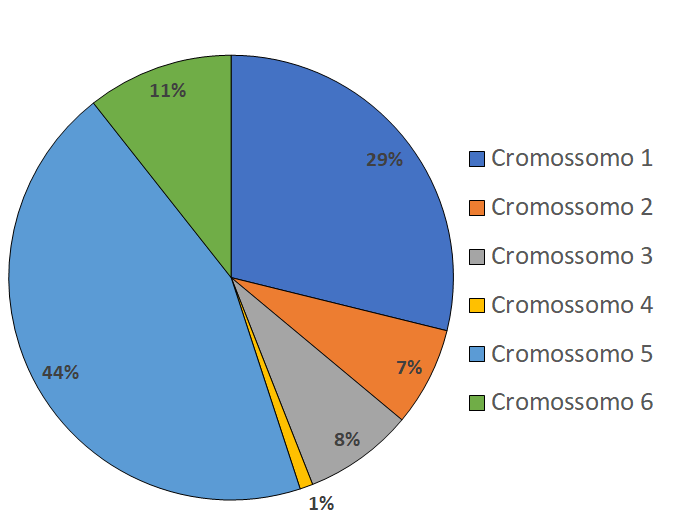
\includegraphics[width=\linewidth]{imagens/exemplo_roleta.png}
			%\caption{Exemplo distribuição em uma roleta viciada}
			\captionof{figure}{Exemplo distribuição em uma roleta viciada}
			\label{fig:exemplo_roleta}
		%\end{figure}
	\end{minipage}
%\end{minipage}
\end{table}

A implementação se torna simples, pois não há necessidade de ordenação dos cromossomos. 

%, e um algoritmo simples para a seleção pode ser visto em \autoref{alg:roleta}, considerando a função \textit{random()} como um gerador de números aleatórios entre 0 e 1. Como pode ser visto, sorteia-se um número entre 0 e o valor da soma das avaliações da população, depois é feito um \textit{loop} iterando pelos valores das avaliações de cada cromossomo e somando a uma variável auxiliar. Ao atingir o valor sorteado, o ultimo individuo que teve seu valor somado a variável auxiliar é retornado.
%
%\begin{algorithm}
%	\LinesNumbered
%	\Entrada{População de cromossomos: populacao}
%	\Saida{Cromossomo selecionado: cromossomo}
%	valor = random() * somaAvaliacao(populacao)\;
%	aux = 0\;
%	i = 1\;
%	\Enqto{aux < valor  {\normalfont \textbf{e}} i <= populacao.tamanho()} {
%			aux = aux + calculaAvaliacao(populacao[i])\;
%			i = i + 1\;
%	}
%	\Retorna{populacao[i-1]}
%	\caption{Roleta viciada}
%	\label{alg:roleta}
%\end{algorithm}

\item[$\bullet$ Amostragem Estocástica Uniforme] \text{}

Uma variação do método da roleta viciada é o Amostragem Estocástica Uniforme (SUS - \textit{Stochastic Universal Sampling}), onde em vez de girar a roleta \textit{N} vezes, é feito apenas um sorteio. O método consiste em alinhar os valores de avaliação dos indivíduos em uma reta contínua, com segmentos proporcionais as avaliações dos cromossomos e normalizados para que a reta tenha tamanho 1. Sorteia-se um número \textit{i} entre 0 e \(1/n\), onde \textit{n} é a quantidade de pais que serão selecionados, e depois são gerados \textit{n} ponteiros para reta na forma \(i + j/n \) com \(j = 0, 2, \dots, n-1 \). Os cromossomos são selecionados conforme esses ponteiros caiam sobre seu segmento correspondente na reta e colocados em uma lista. Os cromossomos da lista devem ser embaralhados ou sorteados de forma uniforme sem reposição para dar sequência com os operadores genéticos. Isso é necessário pois como os segmentos são contínuos, os cromossomos que forem selecionados mais de uma vez estarão na sequência na lista. Esse método, diferente da roleta, garante que cada individuo será selecionado para reprodução um número de vezes no intervalo \(\left[ \lfloor E[i,t] \rfloor , \lceil E[i,t] \rceil \right] \), onde \(E[i,t] = \dfrac{f_i}{\sum f} \cdot n\) é o valor esperado de vezes que o cromossomo \textit{i} será escolhido na geração \textit{t}, com \textit{f} sendo a função de avaliação e \(\sum f\) a soma das avaliações da população. Importante ressaltar que esse método não impede a questão dos superindivíduos dominarem o processo de seleção podendo levar a convergência genética prematura. 

\item[$\bullet$ Seleção por Torneio] \text{}

Nessa forma de seleção é através do método do torneio. Nesse modelo de seleção, são sorteados dois oi mais cromossomos da população com probabilidade uniforme, depois é feito um confronto direto entre os valores de avaliação de cada um, sendo que o que tiver maior valor será o selecionado. Esse mecanismo de seleção evita o favorecimento de indivíduos dominantes da população evitando a convergência genética prematura. Seja \textit{k} a quantidade de cromossomos selecionados para cada rodada do torneio, e \textit{N} o tamanho da população, a probabilidade de seleção de cada um é dada por \(1/N\). Sendo assim a probabilidade de selecionar o pior indivíduo passa a ser \(1/N^k\)), pois para ele ser selecionado para a próxima geração deve ser o único na rodada do torneio. Em testes empíricos esse método de seleção apresentou resultados melhores que o da roleta quando \(k=2\), sendo que não é sensível a questões de escalas da função de avaliação e também ao fato da função de avaliação ser negativa. \cite{Linden2008}

\item[$\bullet$ \textit{Ranking}] \text{}

Outro método é a seleção por \textit{ranking}, que também busca prevenir o convergência genética muito rápida, e consiste em ordenar os indivíduos por suas avaliações e depois usar este ranking para definir o valor esperado de cada um, em vez do valor da avaliação. Assim como no método de torneio, não é necessário se preocupar com a escala da função de avaliação. A relação entre os indivíduos \textit{i} e o \(i+1\) será a mesma independente dos valores avaliados para cada um. 

Para cada cromossomo é classificado com os valores de 1 a \textit{N} indo do pior avaliado para o melhor. O valor esperado de cada cromossomo será dado por \[E[i,t] = \min + (\max - \min) \frac{rank(i,t) - 1}{N - 1} \] onde \(\max\) é o valor esperado para o melhor indivíduo e \(\min\) para o pior. Como há as restrições de \(\max \geq 0\) e \(\sum_i E[i,t] = N\), pois deve-se manter a população, é necessário então que \(1 \leq \max \leq 2\) e \(\min = 2 - \max\).

O valor proposto por Baker é \(\max = 1,1\), e esse método tem a desvantagem de diminuir a pressão seletiva, o que pode levar ao GA uma convergência mais lenta, porém mantém a diversidade garantindo uma melhor exploração do espaço de soluções. Uma forma de manter a pressão seria usar uma função exponencial para definir os valores esperados de cada cromossomo. Seja qual for a forma de mapeamento dos valores esperados, depois pode ser utilizado o método SUS ou da roleta viciada para selecionar os pais da próxima geração.\cite{Mitchell1996}


\item[$\bullet$ Seleção Boltzmann] \text{}

Esse método é inspirado no \textit{simulated annealing}, onde variando a temperatura de forma continua, pode-se controlar a taxa de seleção. O algoritmo inicia com uma temperatura alta, garantindo que todos na população tem maior probabilidade de reprodução, reduzindo a pressão seletiva, e conforme as iterações do algoritmo são executadas, a temperatura é reduzida gradativamente, aumentando assim a pressão seletiva, e restringindo para apenas os melhores continuarem a se reproduzirem. Uma implementação tipica do modelo é \[ E[i,t] = \frac{e^{f_i/T}}{\frac{\sum_j e^{f_j/T}}{N}}\] onde \textit{T} representa a temperatura, e \textit{N} o tamanho da população, assim no denominador da expressão é representada a média da população no instante \textit{t}. \cite{Mitchell1996}

\end{description}

\section{Operadores genéticos}

Definidos como serão a população e a codificação dos cromossomos, além dos métodos de avaliação e seleção do GA, deve-se agora selecionar quais operadores genéticos serão usados. Para cada operador há um parâmetro associado que define uma probabilidade de uso do operador a cada etapa do algoritmo, e os operadores podem ser combinados. Os parâmetros podem ser fixos ou variarem conforme a evolução do algoritmo. Lembrando que com o uso do elitismo, teremos indivíduos que passarão para a próxima geração passar pelos operadores genéticos.

\subsection{Crossover}
O operador mais característico e diferencial do algoritmo genético é o de crossover ou recombinação. É com esse operador que dois cromossomos tem suas características combinadas gerando um novo indivíduo que potencialmente terá avaliação melhor que seus pais. Na literatura temos exemplos de implementação do operador onde há um parâmetro que determina a probabilidade de ser executado o crossover sobre um par de cromossomos selecionados, porém há também exemplos em que sempre é executado o operador. No caso de ser usado esse parâmetro, ele normalmente é alto entre 0,8 e 1, e se após o sorteio ficar definido que não será usado o operador, um dos pais é passado sem alterações para as próximas etapas.

\begin{description}
\item[$\bullet$ Crossover de um ponto] \text{}

Esse é o operador mais simples de crossover, onde é sorteado um ponto de corte dentro do cromossomo para ocorrer a ``quebra'' da sequência dos genes. O cromossomo é formado por uma sequência \textit{n} de genes, e entre esses genes há \(n-1\) pontos de corte que definem as posições onde o cromossomo poderá ser interrompido para ser combinado com outra parte. O processo é feito após a seleção de dois pais, é feito um sorteio para o ponto de corte. Pode ser gerados dois novos indivíduos a partir desse ponto, o primeiro combinando o material genético do pai A a esquerda do ponto de corte e o material genético do pai B a direita do ponto, e o segundo com o inverso. Algumas implementações aproveitam os dois novos indivíduos para a nova geração, outros ainda realizam um sorteio com igual probabilidade de escolha para um dos dois novos cromossomos.

\begin{figure}[ht]
	\centering
	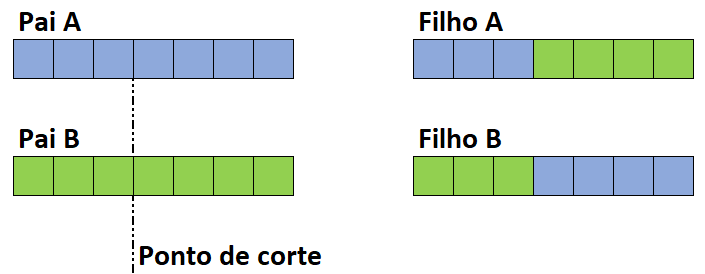
\includegraphics[width=0.75\linewidth]{imagens/exemplo_cross_1pto.png}
	\caption{Crossover com um ponto}
	\label{fig:ex_cross_1pto}
\end{figure}

Existem dois detalhes sobre o crossover de um ponto, primeiro se uma boa solução do problema estiver codificado nos genes extremos do cromossomo, a chance de manter esse dois genes no novo indivíduo reduz muito, pois o novo elemento da população terá a parte inicial do cromossomo ou a parte final somente. Isso também leva ao segundo problema, pois existem uma certa ``preferência'' no método para determinadas posições do cromossomo, já que as partes trocadas entre os pais sempre contém os extremos. \cite{Mitchell1996}.

\item[$\bullet$ Crossover de dois ou mais pontos] \text{}

Para melhorar as questões levantadas pelo crossover de um ponto, surgiram as derivações para terem mais pontos de corte no operador. O processo se mantém o mesmo, no entanto em vez de sortear um ponto de corte para executar as trocas de material genético, são sorteados dois ou mais pontos, e os cromossomos pais tem então suas sequências de genes intercaladas entre esses pontos de corte. Um exemplo para dois pontos é apresentado na \autoref{fig:ex_cross_2pto}.

\begin{figure}[ht]
	\centering
	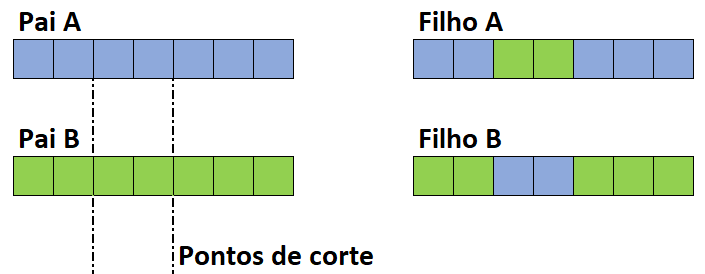
\includegraphics[width=0.75\linewidth]{imagens/exemplo_cross_2ptos.png}
	\caption{Crossover com dois ponto}
	\label{fig:ex_cross_2pto}
\end{figure}

Fazendo o crossover em  mais pontos diminuí os problemas encontrados quando utilizado apenas um ponto de corte. Aumenta-se a chance de manter os genes que estejam em locus distantes na sequência do cromossomo que contribuem para boa avaliação do indivíduo, e diminui-se um pouco o detalhe de uso dos extremos, pois pode-se combinar apenas a parte central de um dos pais.

\item[$\bullet$ Crossover uniforme] \text{}

Esse operador é capaz de combinar qualquer esquema presente nos cromossomos. O conceito de esquemas será melhor explorado na \autoref{sec:esquemas}, mas para o entendimento do crossover, o esquema pode ser considerado como uma máscara para os genes do cromossomo, fixando alguns desses genes e deixando outros livres. Considerando que os genes fixos no esquema são os responsáveis bela boa avaliação do cromossomo, dependendo da distância das posições desses genes na sequência foi visto que os operadores de crossover usando pontos de cortes podem interromper mais facilmente esses esquemas. Com o crossover uniforme esse efeito é minimizado, permitindo que todos os esquemas tenha probabilidade iguais de serem transmitidos aos filhos. O exemplo simplificado do operador pode ser visto em \autoref{fig:ex_cross_unif}
	
	\begin{figure}[ht]
		\centering
		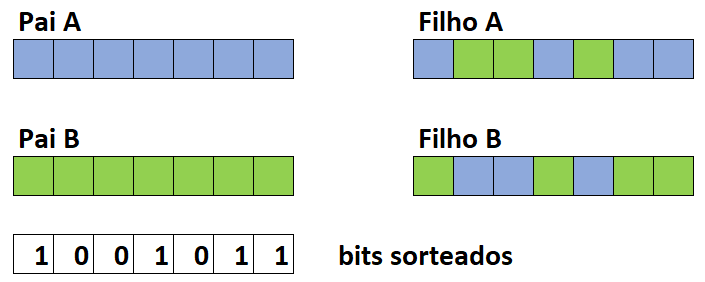
\includegraphics[width=0.75\linewidth]{imagens/exemplo_cross_uniforme.png}
		\caption{Crossover uniforme}
		\label{fig:ex_cross_unif}
	\end{figure}

A diferença com relação aos operadores de combinação anteriores se deve ao fato de que é feito um sorteio dos valores 1 ou 0 com iguais probabilidades para cada posição do cromossomo criando uma sequência binária. Utiliza-se então o resultado do sorteio para definir se será usado o gene do pai A ou do B. Como todas as sequências tem iguais probabilidades de ocorrerem, justifica-se o fato de que os esquemas passam a ter a mesma probabilidade de se manterem durante a reprodução.

\citeauthor{Mitchell1996} menciona uma outra forma de realizar o operador de crossover uniforme, onde seguindo o mesmo raciocínio dos pontos de cortes, onde se realiza um primeiro sorteio para decidir por qual pai começa a construção do filho, e para cada posição do gene é feito um novo sorteio com igual probabilidade para decidir se continua copiando a sequência do pai atual ou se passa a copiar do outro pai, alcançando os mesmos resultados do procedimento descrito anteriormente.

\item[$\bullet$ Crossover baseado em maioria] \text{}

O ultimo operador de crossover apresentado será um que combina vários pais simultaneamente, e não é muito utilizado pois pode levar a convergência genética muito rápido. O conceito por trás desse operador é selecionar \textit{z} pais com \(3 \le z \le N\), sendo \textit{N} tamanho da população, e depois definir para cada gene o valor correspondente a maioria. Alternativamente pode ser feito de forma a calcular uma distribuição para cada gene baseado nos valores encontrados no \textit{z} cromossomos, e depois realizando uma seleção nos moldes da roleta viciada para decidir qual gene utilizar. Esse crossover acaba gerando mais um parâmetro para o algoritmo, pois é necessário definir qual o valor de \textit{z}
 
\end{description}

Os operadores descritos podem em geral serem usados com qualquer tipo de codificação, em especial com codificações binárias seu uso são imediatos. Para algumas outras codificações ajustes são necessários. Para representações com reais paras os genes, ou de grafos como na programação genética, os operadores de crossover que usam pontos de corte ou o uniforme funcionam normalmente, pois definido os pontos de corte basta executar os intercâmbios dos valores situados entre eles. 

Para cromossomos baseados em ordem, isto é, a ordem da sequência apresentada no cromossomo que representa o fenótipo do indivíduo e consequentemente sua avaliação, usar o crossover de um ponto ou mais pode gerar um problema. Como o operador se baseia na posição dos genes para fazer a concatenação, e nesse tipo de cromossomo as posições dos genes mudam, é necessário adaptar o operador. A forma mais simples de realizar essa adaptação é, em vez de intercambiar diretamente os valores entre os pontos de corte, mantém-se os valores de um dos pais selecionado, mas utiliza-se a ordem para esses valores encontradas no segundo pai. Por exemplo na \autoref{fig:ex_cross_ordem}, podemos ver que o pai A possui na região entre os dois pontos de corte a ordem 7 - 1, e esses mesmos valores estão na ordem 1 - 7 no pai B, assim o operador muda a ordem dos valores nesse pedaço para ficar com a mesma ordem do pai B e o resultado é visto no filho A. No filho B o inverso ocorre, sendo que na região de corte é usada a ordem que os valores aparecem no pai A. Pode ser feita uma adaptação análoga para o crossover uniforme. Para o operador baseado em maioria, pode ser feito inciando o primeiro item da sequência pela maioria presente nos pais selecionados, e nas demais posições ir pela maioria encontrada nos pais que seguem o gene escolhido anteriormente.

\begin{figure}[ht]
	\centering
	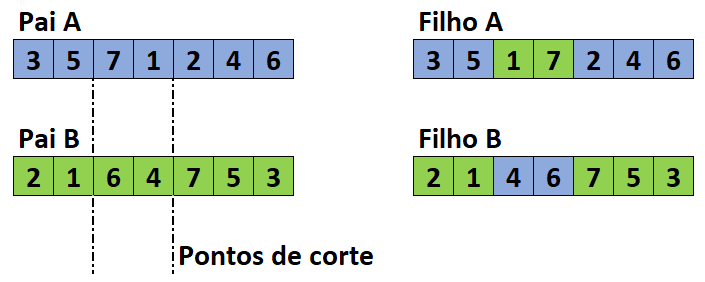
\includegraphics[width=0.75\linewidth]{imagens/exemplo_cross_ordem.png}
	\caption{Crossover com codificação por ordem}
	\label{fig:ex_cross_ordem}
\end{figure}

Quando a codificação for baseada em números reais, o operador de crossover pode ser modificado para em vez de escolher um dos dois valores do gene presentes nos pais, considerar um deles como mínimo e o outro como máximo e realizar um sorteio uniforme no intervalo para o valor do gene. Isso irá gerar filhos bem distintos dos pais, aumentando o aspecto de \textit{exploration} do algoritmo.

\subsection{Mutação}
O operador de mutação é responsável em aumentar o aspecto de \textit{exploration} do GA, e através dele que é possível explorar novas soluções ainda não testadas. Existe um parâmetro associado a esse operador referente a taxa de mutações presentes no algoritmo, sendo que essa taxa usada é um valor baixo na ordem de 0,5\%. A taxa deve ser baixa, pois quanto maior for, mais o algoritmo irá se assemelhar a uma busca randômica. Portanto com probabilidades de mutação nessa ordem garante apenas que novas soluções serão apresentadas quando o algoritmo já estiver convergindo, e assim representa uma alternativa caso o GA estiver convergindo para um máximo local.

O procedimento é simples, para cada gene é feito um sorteio com a probabilidade determinada para a taxa de mutação, caso o sorteio tenha um resultado positivo, o gene em questão será modificado. Essa modificação depende do tipo de codificação que foi utilizado. Para codificação binária há duas opções, inverte-se o estado do bit que deve sofrer a mutação, ou pode-se sortear um novo bit com probabilidade igual para 0 ou 1. Usando essa segunda forma, a taxa de mutação resultante será \(p_m \cdot 0,5\), onde \(p_m\) é o parâmetro de mutação escolhido.

Sobre a codificação binária, existe um detalhe sobre o operador mutação. Como cada bit tem uma significância para o parâmetro que representa do problema, dependendo do bit que for modificado pode representar ``saltos'' maiores ou menores no espaço de soluções e consequentemente nos valores da avaliação. Algumas formas foram propostas para contornar esse dilema, uma seria definir que o \(p_m\) seja proporcional à significância do bit que será modificado. Outra forma seria primeiro transformar a representação binária na variável do problema, realizar uma mutação sobre esse valor, e depois transformar de volta a variável para binário.

Para codificações em inteiro ou em reais, a mutação será na forma de um sorteio sobre o valor do gene. Esse pode usar alguma distribuição conhecida para toda a faixa dos valores que a variável pode assumir, ou usar uma distribuição normal para definir um valor de desvio para a variável e condicionando o resultado para ficar nos limites, ou como visto anteriormente na \autoref{sec:avaliacao}, permitir esse valores fora das restrições que serão penalizados pela função de avaliação.

As mutações para codificações que usam ordem podem ser feita de duas formas. A primeira se um gene deverá ser modificado, sorteia-se outro gene aleatoriamente e é feita a permutação dos dois. Na segunda forma defini-se dois pontos no cromossomo e é feita ou uma mistura dos elementos entre esses dois pontos, ou inverte-se a ordem entre esses dois pontos.

Para cromossomos baseados em grafos, ou árvores, a sugestão é remover o ramo selecionada para mutação, e gerar um novo aleatório, seguindo o mesmo processos usado para gerar a população inicial.

É comum usar para o parâmetro de taxa de mutação, um valor variável, que pode ir aumentando a cada iteração do algoritmo, permitindo assim que conforme vai se atingindo a convergência genética, o GA não perca sua característica de \textit{exploration}, buscando soluções totalmente novas.

\subsection{Outros operadores}
Existem outros operadores menos usados no algoritmo como por exemplo o de inversão proposto por Holland e alguns que operam sobre como são formados os pares para reprodução.

\citeauthor{Holland1992} propôs um operador que inverte parte da sequência do cromossomo, isso pois percebeu a questão do crossover de um ponto que têm uma maior probabilidade em interromper esquemas com genes mais afastados na sequência. Esse operador é inspirado pelo que acontece na genética real, onde a função do gene não depende da sua posição, portanto invertendo parte do cromossomo, sua essência seria mantida. Para adaptar esse operador no GA, além do valor do gene, o cromossomo deve armazenar qual a sua posição original também, o que acarreta uma maior custo computacional. O funcionamento básico do operador é selecionar dois pontos aleatórios no cromossomo, e inverter a ordem dos genes encontrados nesse intervalo. Quando foi realizar o crossover, como os pais selecionados podem ter a ordem dos genes alteradas, utiliza-se um deles como referência e ordena-se o segundo da mesma forma, assim o crossover não correrá o risco de repetir genes na concatenação das partes. Testes com inversão foram feitos mas nenhum obteve resultados indicando que o uso desse operador melhora o desempenho do GA. \cite{Mitchell1996}.

Além desse operador, foram feitos alguns experimentos com operadores de seleção que procuram determinar outros fatores na seleção dos pais, como por exemplo não selecionar dois indivíduos que tenham o genótipo parecido, evitando assim convergência genética prematura e buscando que a combinação entre pais geram filhos diferentes dos encontrados na população até o momento.

Também existem as versões dos operadores apresentados para cromossomos diplóides, onde o genótipo possui um par de cromossomos, sendo que deve ser utilizado o aspecto de dominância dos alelos para definir o fenótipo. A maior diferença está no operador de crossover, pois por serem indivíduos diplóides, ocorre primeiro a separação do par de cromossomos em gametas, feito o crossover e depois recombinação entre os gametas dos pais selecionados. Em \cite{Goldberg1989} é possível verificar uma análise mais detalhada sobre esse assunto.

\section{Fundamentos teóricos}
\subsection{Esquemas}
\label{sec:esquemas}
O conceito de esquema (\textit{schema} ou \textit{schemata}) foi primeiro definido por \citeauthor{Holland1992}, em uma tentativa de especificar por qual razão o algoritmo genético funciona e pode ser eficiente. Foi apresentado também por \citeauthor{Goldberg1989} como teorema fundamental do GA, e ficou conhecido de Teorema dos Esquemas (\textit{Schema Theorem}). Por trás desse conceito, Holland ainda explica a teoria do paralelismo implícito presente no algoritmo razão da qual ele apresentar certa eficiência se comparado a outros algoritmos.

Para explicar o conceito primeiro define-se que o cromossomo é uma sequência, de comprimento \textit{l}, de genes que podem ter os alelos presentes no alfabeto \textit{V}. Para simplificar as definições e cálculos e sem perda de generalidade, foi escolhido um alfabeto binário \(V = \{0, 1\}\) e os cromossomos são portanto sequências binárias. O esquema funciona como um gabarito ou \textit{template} definindo assim subconjuntos de todos os possíveis indivíduos. Para realizar tal gabarito o esquema usa um outro elemento considerado um coringa, que representa uma posição no cromossomo que não importa (\textit{don't care}). Assim para o alfabeto binário utilizado o alfabeto para os esquemas pode ser definido como \(V+ = {0, 1 , *}\), sendo \textit{*} nosso valor coringa. Exemplo, para uma população de cromossomos com \(l=8\), o esquema \(H=**11*0*1\) tem os indivíduos com cromossomos \(A_1=00110001\) e \(A_2=10111011\) como representantes desse esquema e são chamados de instâncias de \textit{H}. Assim se tivermos cromossomos binários com comprimento \textit{l} existirão \(2^l\) combinações possíveis de cromossomos e \(3^l\) combinações de esquemas.

Existem duas características importantes sobre os esquemas, uma delas é sua \textbf{ordem}, denotada por \(o(H)\), que define quantas posições possuem valor fixo no esquemas, isto é, quantas posições no esquema são diferentes de \textit{*}. No exemplo anterior \(H=**11*0*1\) possui ordem 4(\(o(**11*0*1) = 4\)). Outra característica é o \textbf{tamanho} do esquema (\textit{defining length}), denotado por \(\delta(H)\), que é calculado como a diferença entre as posições do ultimo valor definido no esquema e do primeiro definido. Por exemplo para o esquema \(011*1***\) seu tamanho é 4, pois o ultimo valor definido está na posição 5 e o primeiro na posição 1 (\(\delta(011*1***) = 4\)). 

Goldberg usou o simbolo \textit{H} pois o esquema define um hiperplano do espaço de dimensão \textit{l} que representa as sequências binárias de comprimento \textit{l}. Considerando sequências binárias e esquemas de comprimento \(l=3\), é possível desenhar a representação dos hiperplanos de forma geométrica, que pode ser visto na \autoref{fig:schema_hyperplane}. Os vértices são esquemas de ordem 3, as linhas de ordem 2 e os planos de ordem 1.

\begin{figure}[ht]
	\centering
	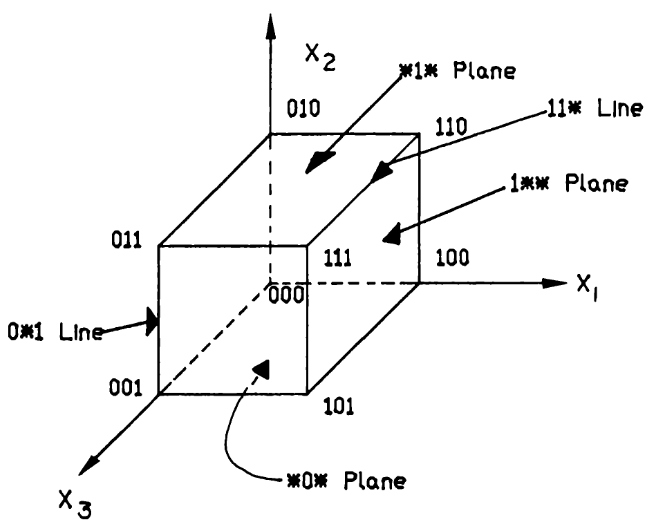
\includegraphics[width=0.75\linewidth]{imagens/schema_hyperplane.png}
	\caption{Representação dos esquemas como hiperplanos em um espaço tridimensional. \cite{Goldberg1989}}
	\label{fig:schema_hyperplane}
\end{figure}

Avaliando os novos conceitos, pode ser verificado que quanto maior for o tamanho de um esquema (\(\delta(H)\)), maior será sua probabilidade de ser desfeito com os operadores genéticos de crossover, e quanto maior sua ordem, maior será a probabilidade do operador de mutação também destruí-lo. Apesar da probabilidade de modificar alguns dos esquemas presentes e que foram bem avaliados, pois os operadores serão aplicados aos cromossomos selecionados e portanto que possuem melhor avaliação me média, existe a chance de com isso encontrar esquemas que responderão melhor ainda para o problema em questão. 

Como esquemas de ordem e tamanho maiores estão mais sujeitos a serem destruídos, os esquemas mais curtos e que mais contribuem para a avaliação dos cromossomos, tendem a ser preservados, e esses constituem os blocos de construção (\textit{building blocks}) citados por \citeauthor{Goldberg1989}.

O que \citeauthor{Holland1992} indica como paralelismo intrínseco se atribui ao fato, de que apesar do algoritmo estar avaliando \textit{n} indivíduos contido na população na geração presente, ele está também avaliando de forma implícita um número bem maior de esquemas. Qualquer sequência binária de comprimento \textit{l} é uma instância de \(2^l\) esquemas. Por exemplo a sequência 11, é uma instância dos seguintes esquemas: **, 1*, *1 e 11. Estendendo para a população de tamanho \textit{n} existem portanto um total de até \(n \cdot 2^l\) esquemas, assim o total de esquemas em determinada população será um valor entre \(2^l\), caso todos os cromossomos sejam iguais, e \(n \cdot 2^l\), caso todos diferentes. Por essa razão o GA avalia uma quantidade de esquemas maior do que a quantidade de indivíduos presentes na população.

\subsection{Teorema fundamental do GA}
A definição do teorema dos esquemas de acordo com \cite{Linden2008} é "o GA tende a preservar com o decorrer do tempo aqueles esquemas com maior avaliação média e com menores ordem e tamanho, combinando-os como blocos de armar de forma a buscar a melhor solução". 

O teorema pode ser verificado através da estimação do aumento ou diminuição das instâncias dos esquemas presentes na população. Consideremos uma população \(\Omega\) de tamanho \textit{N} de cromossomos com codificação binária e comprimento \textit{l}. Seja \textit{H} um esquema que tenha ao menos uma instância na população na geração \textit{t}, e \(m(H, t)\) o número de instâncias de \textit{H} no instante \textit{t}. Definimos \[\hat{u}(H,t) = \frac{\sum\limits_{x \in H}f(x)}{m(H,t)}\]
onde \textit{x} é um indivíduo na população, e \(f(x)\) é a função de avaliação. Assim \(\hat{u}(H,t)\) é a média das avaliações das instâncias de \textit{H} no instante \textit{t}.

Relembrando que a probabilidade de um indivíduo ser escolhido para seleção com o método da roleta viciada é definido por \(p(i) = f(i) / \sum_{j=0}^{N}{f(j)}\), com \(i = 1,2,\dots,n\). Sendo \(n(i,t)\) a quantidade de vezes que o cromossomo \textit{i} é selecionado na população na geração \textit{t}, o valor esperado de \textit{n} será \(E[n(i,t)] = N \cdot p(i)\). Se \(\overline{f}(t) = \sum_{i \in \Omega} {f(i)} / N\) é a média das avaliações da população no instante \textit{t}, o valor esperado de \(n(i,t)\) pode ser expresso como \(E[n(i,t)] = f(i) / \overline{f}(t)\)

O valor esperado da quantidade de instâncias de \textit{H} em \(t+1\) considerando apenas a seleção descrita e sem usar os operadores de crossover e mutação será dado por:
\begin{align}
	E[m(H,t+1)] &= \frac{\sum\limits_{x \in H} {f(x)}}{\overline{f}(t)} \nonumber \\
				&= \frac{\hat{u}(H,t)}{\overline{f}(t)} m(H,t)
\label{eq:valor_esperado_H}
\end{align}

Assim é verificado que a quantidade de instâncias do esquema \textit{H} na próxima geração depende diretamente da média das avaliações das instâncias do esquema na geração atual e pode ser concluído que esquemas com avaliação maior que a média irão aumentar ao passo que os avaliação menor diminuirão.

Como visto antes, os operadores de crossover e mutação podem tanto construir como destruir as instâncias do esquema \textit{H}, e que a probabilidade de destruir é proporcional as características do esquema dado pela ordem (\(o(H)\)) e pelo tamanho (\(\delta(H)\)). Considerando apenas o fato destrutivo dos operadores, para o caso do crossover de ponto único, com \(p_c\) sendo a probabilidade de ser aplicado, o limite inferior da probabilidade de sobrevivência do esquema pode ser estimado como:
\[S_c(H) \ge 1 - p_c \frac{\delta(H)}{l - 1}\] % parte depois do 1 - é o limite superior da probabilidade de destruir ele, e 1 - p_destroy e a probabilidade de sobreviver%
e pela equação é verificado que quanto menor o tamanho do esquema, maior sua probabilidade de sobrevivência.

Já para o operador de mutação, considerando \(p_m\) como a probabilidade de um bit sofrer mutação, a probabilidade de sobrevivência do esquema é dada por:
\[S_m(H) = (1 - p_m)^{o(H)}\]
e novamente quanto menor a ordem do esquema, maior probabilidade de sobrevivência.

Por fim, a \autoref{eq:valor_esperado_H} pode ser alterada para definir um limite inferior dado por:
\begin{equation}
E[n(H,t+1)] \ge \frac{\hat{u}(H,t)}{\overline{f}(t)} m(H,t)\left( 1 - p_c \frac{\delta(H)}{l - 1} \right) \left[(1 - p_m)^{o(H)} \right]
\label{eq:schema_theorem}
\end{equation}
A \autoref{eq:schema_theorem} define o Teorema dos Esquemas proposto por \citeauthor{Holland1992} e que pode ser visto também em \citeonline{Goldberg1989}. 

\subsection{Two-armed bandit}
\citeauthor{Holland1992} menciona que a adaptação possui uma tensão entre os componentes de \textit{exploitation} e \textit{exploration}, e que a análise de esquemas demonstrava, assumindo certas condições, que o GA atingi um certo equilíbrio próximo do ótimo. A permutação entre os dois podem ser comparados com o \textit{``Two-armed bandit problem''}\footnote{Uma máquina caça-níquel é também conhecida como \textit{One-armed bandit}}.\cite{Mitchell1996}

O problema é descrito como um jogador com \textit{N} moedas e uma máquina caça-níquel com duas alavancas, sendo que uma delas(\(A_1\)) paga com média \(\mu_1\) e desvio-padrão \(\sigma_1\) e a outra(\(A_2\)) paga com média \(\mu_2\) e desvio-padrão \(\sigma_2\). Esses valores não variam, são independentes e são desconhecidos ao jogador. O objetivo do jogador é maximizar os lucros, porém como não tem informações sobre qual das alavancas paga mais, só pode estimar realizando jogadas nas duas. 

\citeauthor{Mitchell1996} descreve uma solução simples para o problema seguindo o que foi proposto por \citeauthor{Holland1992} e que pode ser visto em detalhes em \citeonline{Holland1992}. Considerando sem perda de generalidade que \(\mu_1 > \mu_2\), ou seja, a alavanca \(A_1\) paga mais que a \(A_2\), e sendo \(A_h(N, N-n)\) e \(A_l(N,n)\) as alavancas com maior e menor valores pagos observados respectivamente, após \textit{N} tentativas, sendo \(N-n\) tentativas usadas em \(A_h\) e \textit{n} tentativas na \(A_l\). O que se busca é o valor \(n = n^*\) que maximize o lucro. A melhor estratégia seria colocar as \textit{N} apostas na alavanca que paga mais, porém como ela não é conhecida isso não é possível.

Duas possibilidades podem ocorrer, ou \(A_l\) corresponde a pior alavanca e nesse caso houve prejuízo somente nas \(n\) apostas feitas em \(A_l\) (as perdas dadas por \((N-n)(\mu_1-\mu_2)\)), ou \(A_l\) corresponde a melhor alavanca e então houve prejuízo nas \(N- n\) apostas colocadas em \(A_h\) (perdas dadas por \(n(\mu_1-\mu_2)\)). Seja \textit{q} a probabilidade de \(A_l\) ser na verdade a melhor alavanca \(A_1\), isto é, \(q = P(A_l(N,n) = A_1)\), assim as perdas \(L(N-n,n)\) após \textit{N} tentativas é dado por:

\begin{equation*}
L(N-n,n) = q(N-n)(\mu_1-\mu_2) + (1-q)n(\mu_1-\mu_2)
\end{equation*}

Como o desejado é \(n = n^*\) que minimiza essa função (ou seja maximiza o lucro), tomando a derivada com relação a \textit{n} e igualando a zero.
\begin{equation*}
\frac{dL}{dn} = (\mu_1-\mu_2)\left( 1 - 2q + (N-2n)\frac{dq}{dn}\right) = 0
\end{equation*}

Que para ter uma solução é necessário expressar \textit{q} em função de \textit{n}. Sejam \(S_1^n\) a soma recebida pelas apostas em \(A_1\) e \(S_2^{N-n}\) a soma recebida pelas apostas em \(A_2\). Então \textit{q} pode ser expresso na forma:

\begin{align}
q 	&= P\left(\frac{S_2^{N-n}}{N-m} > \frac{S_1^n}{n}\right) \nonumber \\
	&= P\left( \left( \frac{S_2^{N-n}}{N-m} - \frac{S_1^n}{n} \right) < 0 \right)
\label{eq:prob_q}
\end{align}

que indica de fato a probabilidade de observar que \(A_2\) pagou mais que \(A_1\). Como \(S_1^n\) e \(S_2^{N-n}\) são variáveis aleatórias, sua diferença também é uma v.a. e a probabilidade descrita em \autoref{eq:prob_q} é a área abaixo da curva de distribuição na parte menor que zero. \citeauthor{Holland1992} aproximou essa probabilidade usando o teorema central do limite assumindo a distribuição normal. Na segunda edição, Holland atribui a correção dessa aproximação para Dan Frantz, que usou a teoria dos grandes desvios(\textit{theory of large deviations}), para aproximar essa probabilidade e chegar ao resultado:

\begin{equation*}
n^* \approx c_1 ln\left( \frac{c_2 N^2}{ln(c_3 N^2)} \right)
\end{equation*}

onde \(c_1\), \(c_2\) e \(c_3\) são constantes positivas. Rearranjando os termos obtêm-se:

\begin{equation*}
N - n^* \approx e^{n^*/2c_1} \sqrt{\frac{ln(c_3 N^2)}{c_2}} - n^*
\end{equation*}

Conforme \(n^*\) aumenta, o termo exponencial domina a equação, e pode-se aproximar mais ainda obtendo:

\begin{equation*}
N - n^* \approx e^{cn^*}
\end{equation*}

que indica em resumo que o valor ótimo de apostas \(N-n^*\) feitas à melhor alavanca observada deve aumentar exponencialmente conforme o número de apostas feitas na pior alavanca observada. \cite{Mitchell1996}

O que o Teorema dos Esquemas sugere é que da mesma forma que o problema descrito \textit{``two-armed bandit''} que pode ser estendido a um problema com \textit{k} alavancas(\textit{``k-armed bandit''}), o GA aumenta de forma exponencial as tentativas feitas com os melhores esquemas observados com relação as tentativas feitas aos piores esquemas. \citeauthor{Goldberg1989} indica que na verdade o GA deve ser comparado a uma composição de \textit{k-armed bandits}.

\citeauthor{Mitchell1996} faz uma ressalva com a comparação com relação ao fato de que no caso do \textit{two-armed bandit}, as alavancas são independentes, que não é o caso do GA, pois os esquemas interagem entre eles, pois por exemplo, o valor observado de retorno do esquema \(111*\ldots*\) tem influência sobre o valor observado do retorno de \(1***\ldots*\).

\subsection{O GA como uma cadeia de Markov}
O teorema dos esquemas versa sobre a evolução dos esquemas presentes no algoritmo, porém para tentar determinar exatamente fatores como a distribuição da população, das avaliações e da convergência do algoritmo conforme as iterações, foram procurados outros modelos matemáticos para determinar o comportamento do GA. Um desses modelos descritos por \citeauthor{Nix1992}, modela o GA na forma de uma cadeia de Markov, para uma população finita. Assim o estado atual é definido pela presente população, que através de uma matriz de transição \textit{Q} define a probabilidade de ir para uma nova população dada a atual.

Seja o espaço de soluções definido por \(\Omega\) formado por cromossomos codificados como sequências binárias de comprimento \textit{l}, assim \(r=2^l\) define a quantidade de soluções possíveis, e seja \textit{P} uma população de elementos de \(\Omega\) de tamanho \textit{n}. \textit{N} é a quantidade de possíveis populações que podem ser formadas e pode ser calculado como:
\[N = \binom{n+2^l-1}{2^l-1}\]
que de fato é a combinação com repetição de \textit{n} elementos de um conjunto com \(2^l\) elementos.

Define-se a matriz \textit{Z} com tamanho \(r\times N\) cuja as colunas representam todas as possíveis populações de tamanho \textit{n}. Cada coluna é um vetor coluna das incidências de cada elemento \textit{y} de \(\Omega\) na população \(P_i\), isto é,  cada elemento \(z_{y,i}\) representa o número de ocorrências do indivíduo \textit{y} na população \(P_i\), com \textit{y} sendo o indexador do indivíduo começando com 0. A matriz \textit{Z} define assim os possíveis estados da cadeia de Markov.

Agora seja \textit{Q} a matriz de transição de tamanho \(N \times N\), onde \(Q_{i,j}\) é a probabilidade de a partir da população \(P_i\) passar para a população \(P_j\). Para determinar a as probabilidades de transição, defini-se \(p_i(y)\) como a probabilidade de do indivíduo \textit{y} ser gerado a partir de \(P_i\) através dos operadores genéticos de seleção e recombinação(crossover e mutação). Na próxima população \(P_j\), \textit{y} está presente o número de vezes determinado em \(z_{y,j}\), e para determinar a probabilidade, Nix e Vose enumeraram as formas possíveis de gerar as sequências presentes em \(P_j\).

A quantidade de formas de selecionar \(z_{0,j}\) vezes o indivíduo 0 dentro da população de tamanho \textit{n} é dado por \(\binom{n}{z_{0,j}}\), e sobram \(n - z_{0,j}\) posições na população para serem preenchidas. Seguindo para o indivíduo 1, a quantidade de formas de selecionar ele \(z_{1,j}\) vezes é definido por \(\binom{n-z_{0,j}}{z_{1,j}}\). Continuando da mesma maneira, o total de combinações para todas os indivíduos é dado por:
\begin{equation*}
\binom{n}{z_{0,j}}\binom{n-z_{0,j}}{z_{1,j}}\cdots \binom{n-z_{0,j}-\cdots -z_{2^l-2,j}}{z_{2^l-1,j}} = \frac{n!}{z_{0,j}!z_{1,j}!\cdots z_{2^l-1,j}!}
\end{equation*}

Como a probabilidade de produzir a quantidade certa do indivíduo \textit{y} na população \(P_j\) a partir da população \(P_i\) é dado por:
\[ \prod_{y=0}^{2^l-1}\left(p_i(y)\right)^{z_{y,j}} \]

A probabilidade de produzir \(P_j\) a partir de \(P_i\) fica definido como a distribuição multinomial dada por:
\begin{equation*}
Q_{i,j} = \frac{n!}{z_{0,j}!z_{1,j}!\cdots z_{2^l-1,j}!} \prod_{y=0}^{2^l-1}\left(p_i(y)\right)^{z_{y,j}} = n!\prod_{y=0}^{2^l-1} \frac{\left(p_i(y)\right)^{z_{y,j}}}{z_{y,j}!}
\end{equation*}

Para calcular a probabilidade \(p_i(y)\) no artigo de \citeonline{Vose1991PunctuatedEI} são derivados duas matrizes, \textit{F} que define a avaliação dos indivíduos em sua diagonal principal e \textit{M} que define a recombinação do algoritmo genético simples. Seja \(\overrightarrow{\phi}_i\) o vetor coluna que representa a população \(P_i\) e portanto é uma das colunas de \textit{Z}, e define-se \(\left| \overrightarrow{\phi}_i \right|\) como a soma dos elementos do vetor. Dessa forma a proporção dos indivíduos \textit{y} na população \(P_i\) é dada por \((\overrightarrow{\phi}_i / \left| \overrightarrow{\phi}_i \right| )_y\).
A probabilidade de \textit{y} ser selecionado é dado por
\[\left( \frac{F \overrightarrow{\phi}_i}{\left| F \overrightarrow{\phi}_i \right|} \right)_y\]
e o valor esperado da proporção de \textit{y} na próxima geração dado por
\[\left[ M \left( \frac{F \overrightarrow{\phi}_i}{\left| F \overrightarrow{\phi}_i \right|} \right) \right]_y\]
e como \(p_i(y)\) é equivalente a proporção esperada de \textit{y}, a matriz de transição então pode ser escrita como 

\begin{equation*}
Q_{i,j} = n!\prod_{y=0}^{2^l-1} \frac{\left[ M \left( \frac{F \overrightarrow{\phi}_i}{\left| F \overrightarrow{\phi}_i \right|} \right)_y \right]^{z_{y,j}}}{z_{y,j}!}
\end{equation*}

Assim a cadeia de Markov fica definida com \textit{Z} sendo a matriz de estados, e \textit{Q} a matriz de transições. Com base nas propriedades das cadeias de Markov, \citeauthor{Nix1992} derivaram alguns resultados importantes, como por exemplo, quando \(n \to \infty\), a cadeia converge para iterações de \textit{G}, com probabilidade próxima de 1, onde \(G = F \circ M \). Também mostraram que para \textit{n} suficientemente grande, e se \(G_p\) tem um ponto fixo, o GA tende a ficar o tempo todo com a população correspondente a este ponto. Se \(G_p\) tem mais de um ponto, o GA gasta um tempo fora desses pontos com tendência a 0.\(G_p(\overrightarrow{x}) = M \left( {F \overrightarrow{x}}/{\left| F \overrightarrow{x} \right|} \right) \)

Apesar de lucidar alguns pontos sobre o GA, esses modelos são impraticáveis para predizer modelos reais por serem muitos detalhados e necessitarem de matrizes muito grandes conforme \textit{l} e \textit{n} aumentam.

\subsection{Mecânica estatística}
Uma outra forma de avaliar o GA indicado por \citeauthor{Mitchell1996} é o uso da mecânica estatística, que em vez de procurar determinar como cada parte define o comportamento do algoritmo, procura ver o GA de uma forma mais macroscópica. Um estudo feito sobre esse tema pode ser encontrado no \citeonline{Pruegel-Bennett1994}, onde usaram o modelo de Ising de uma dimensão e o GA para minimizar a energia na grade. O objetivo era verificar e tentar prever o comportamento da distribuição de energia na população conforme as gerações do algoritmo. Para o modelo de uma dimensão, \citeauthor{Pruegel-Bennett1994}, conseguiram gerar uma previsão sobre os dois primeiros momentos, média e variância, da distribuição de energia na população.

Como será visto no \autoref{chap:implementGA} foi escolhido o modelo de Ising com duas dimensões, e será feito uma simulação para verificar o comportamento da distribuição da população durante as gerações do algoritmo, variando alguns dos parâmetros do GA para averiguar quais mudanças causam nos resultados.

\section{Problemas associados ao GA}
\label{sec:problemas_GA}
Existem duas situações conhecidas que levam o GA a ter uma piora de desempenho podendo se tornar ineficiente. Uma delas é chamado de carona (\textit{hitchhiking}), e consiste no fato de que genes vizinhos aos que formam esquemas com alta avaliação, tendem a se manter nas próximas gerações como caronistas. Isso levanta questões sobre o teorema dos esquemas, dando argumentos aos que se opõe a ele. No exemplo de codificação binária, a ocorrência desses bits que pegam caronas se deve ao operador de crossover, que deveria ter seus pontos de corte sorteados de tal forma a precisamente manter somente os bits que geram a alta avaliação no esquema e remover os caronas, mas que dependendo do comprimento das cadeias de bits e dos esquemas passam a ter probabilidade pequena de ocorrerem. 

Outra questão levantada sobre os GAs é com relação aos problemas que foram definidos como enganadores (\textit{deceptives}), que são problemas que apresentam esquemas que não contêm o máximo global com média de avaliação superior aos esquemas que o contêm. \citeauthor{Linden2008} descreve esses problemas como tendo o máximo global em forma de pico cercados por valores de avaliação muito baixos, porém da mesma forma que impõem uma dificuldade ao GA, também será difícil para outros métodos.

\citeauthor{Spall2003} também menciona a questão sobre epistasia, onde genes interagem entre si e combinados produzem um resultado melhor do que avaliados individualmente, o que vai contra a teoria dos blocos de construção de \citeauthor{Goldberg1989}, onde pequenos blocos com alta avaliação garantem ao GA sua eficiência. Na forma do algoritmo genético simples apoiado no teorema dos esquemas, ficou definido que o GA tende a preservar esquemas com menor ordem e tamanho, mas no caso deveria-se preservar esquemas que podem ter o tamanho grande se os genes que interagem ocupam posições distantes no cromossomo.

Mesmo com o GA apresentando alguns problemas, ele pode ser uma opção interessante, principalmente se o conhecimento do problema permitir que esses efeitos sejam reduzidos, como o posicionamento dos genes no cromossomo, ou o uso de outros operadores, como o de inversão que explora novos posicionamentos dos genes, ou usar operadores modificados de crossover, ou de mutação direcionados. Além disso ainda existe a opção de combinar o GA com outros métodos de otimização locais, por exemplo, usar o método de \textit{hill-climbing} na fase de mutação.


% ---
% Capitulo explicando modelo de Ising
% ---
%\include{isingModel}

% ---
% Capitulo explicando implementacao
% ---
% ---
% Este capítulo, apresenta os conceitos sobre o algoritmo genético
% ---

\chapter{Implementação do algoritmo genético}
\label{chap:implementGA}

Para implementação do algoritmo foi utilizado a linguagem de programação Java, e os testes feitos com dois problemas distintos. As avaliações foram feitas através de gráficos e estatísticas geradas no R.

\section{Implementação inicial}
Os testes começam sobre um modelo simples usando codificação binária para representar duas variáveis reais \textit{x} e \textit{y} com valores no intervalo \([-100,100]\), e 15 bits de comprimento. A conversão é feita usando um fator \textit{C} definido por \(C = \dfrac{200}{2^{15} - 1}\) que multiplicado pela representação binária transformada para o inteiro \textit{i} e somado ao valor mínimo, apresenta o valor real da variável, com resolução definida pelo fator,
\(x = C \cdot i_x - 100\). O cromossomo é formado por uma sequência de 30 bits, 15 para cada variável, concatenados na forma de um vetor (Em Java será utilizado os conceitos de Listas por serem mais versáteis com relação aos elementos que podem ser guardados e manipulados). A função que deve ser maximizada, que será a mesma de \textbf{avaliação}, é dada pela equação seguinte e apresenta o gráfico visto na \autoref{fig:grafico_teste1}: 
\[f(x,y) = \left| x \cdot y \cdot \sin\left(\frac{\pi \cdot y}{4}\right) \right|\] 
É possível ver que a função possui 4 pontos máximos definidos dentro do domínio, e utilizando o R para encontrar o máximo da função em um desses pontos, foi obtido os seguintes resultados: \(x = 100\), \(y = 98,01654\) e \(f(x,y) = 9800,827\). O ponto com é critico de ser encontrado pelo fato de possuir vários máximos locais dentro do domínio. Para comparação dos resultados do GA, sempre será executado uma busca aleatório com a quantidade de pontos gerados equivalentes a \(n * T\), onde \textit{n} é o tamanho da população definido como parâmetro do GA e \textit{T} o total de gerações que o algoritmo será executado.

%\begin{figure}[ht]
%	\centering
%	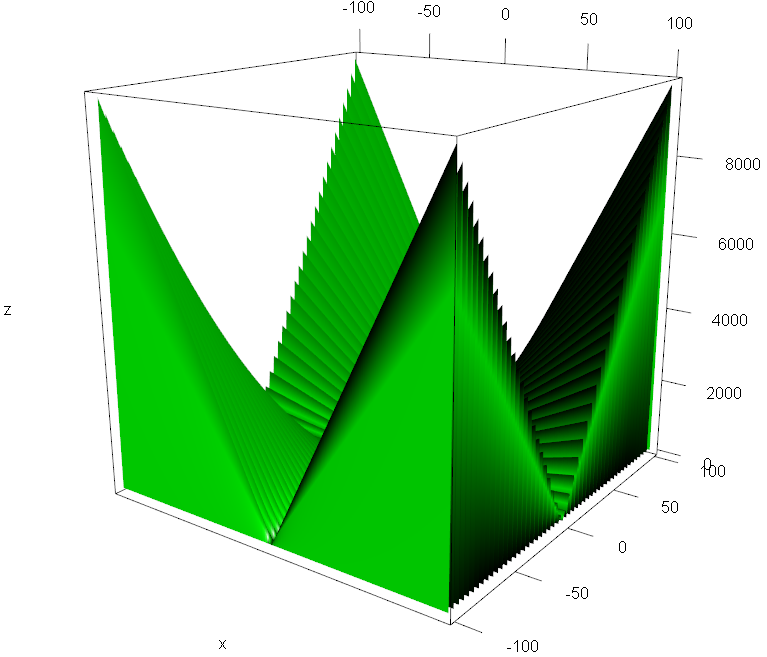
\includegraphics[width=1.1\linewidth]{imagens/teste1.png}
%	\caption{Gráfico da função de avaliação}
%	\label{fig:grafico_teste1}
%\end{figure}

\begin{figure}[ht]
	\centering
	\begin{subfigure}[b]{0.47\linewidth}
		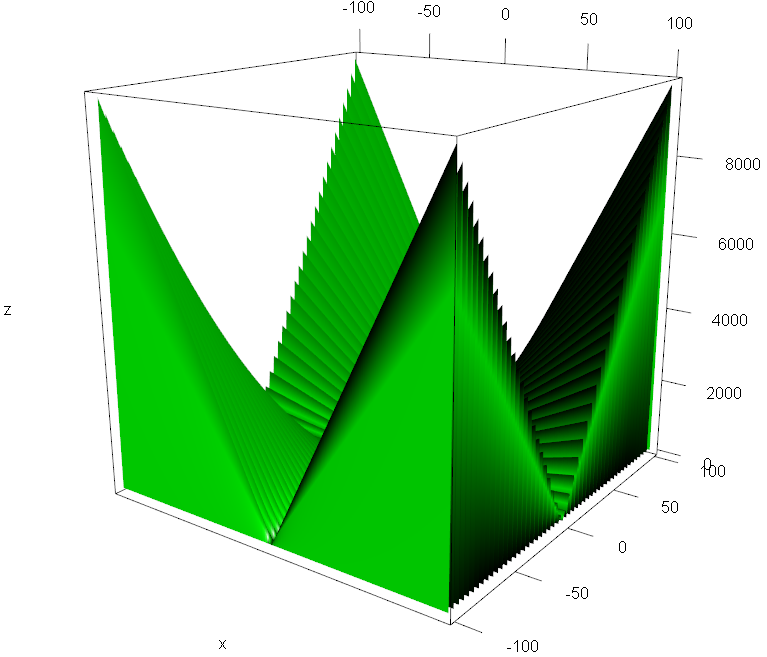
\includegraphics[width=\linewidth]{imagens/teste1.png}
		\caption{Gráfico no domínio completo}
	\end{subfigure}
	\begin{subfigure}[b]{0.47\linewidth}
		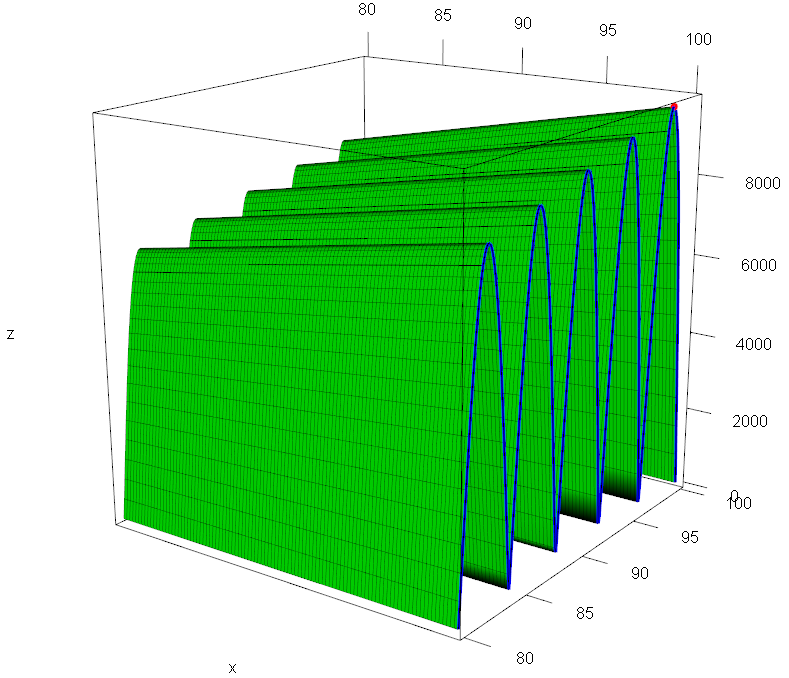
\includegraphics[width=\linewidth]{imagens/teste2.png}
		\caption{Gráfico ampliado em um dos máximos}
	\end{subfigure}
	\caption{Gráfico da função de avaliação}
	\label{fig:grafico_teste1}
\end{figure}

Para esse GA foi utilizado o método de seleção da roleta viciada, com um algoritmo simples que pode ser visto em \autoref{alg:roleta}, considerando as funções \textsf{random()} como um gerador de números aleatórios entre 0 e 1, \textsf{somaAvaliacao()} que soma todos os valores da função de avaliação dos cromossomos da população e \textsf{calculaAvaliacao()} que calcula o valor da função de avaliação de um cromossomo da população. Como pode ser visto, sorteia-se um número entre 0 e o valor da soma das avaliações da população, depois é feito um \textit{loop} iterando pelos valores das avaliações de cada cromossomo e somando a uma variável auxiliar. Ao atingir o valor sorteado, o ultimo individuo que teve seu valor somado a variável auxiliar é retornado.

\begin{algorithm}[h!]
	\LinesNumbered
	\SetKwFunction{somaAvaliacao}{somaAvaliacao}\SetKwFunction{calculaAvaliacao}{calculaAvaliacao}
	\SetKwFunction{random}{random}
	\Entrada{População de cromossomos: $populacao$}
	\Saida{Cromossomo selecionado: $cromossomo$}
	$valor$ = \random() * \somaAvaliacao($populacao$)\;
	$aux$ = 0\;
	$i$ = 1\;
	\Enqto{aux < valor  {\normalfont \textbf{e}} i <= populacao.tamanho()} {
			$aux = aux$ + \calculaAvaliacao($populacao[i]$) \;
			$i = i + 1$ \;
	}
	\Retorna{populacao[i-1]}
	\caption{Roleta viciada}
	\label{alg:roleta}
\end{algorithm}

O operador de crossover testado foi o com único ponto de corte, e seu algoritmo pode ser visto em \autoref{alg:crossover}, sendo \textsf{concatenar()} a função responsável por unir as duas partes dos cromossomos pais e formar um novo cromossomos que é colocado na variável \textit{Filho}. O crossover somente é executado se no sorteio inicial, o valor for menor que \(p_c\). Caso não seja aplicado o operador, é feito uma cópia do \textit{PaiA}.

\begin{algorithm}[h!]
	\LinesNumbered
	\SetKwFunction{concatenar}{concatenar} \SetKwFunction{random}{random}
	\Entrada{Cromossomos: $PaiA$ e $PaiB$; probabilidade de crossover: $p_c$}
	\Saida{Cromossomo: $Filho$}
	\eSe{ \random() <= $p_c$}{
		$corte$ = \random() * $PaiA.tamanho()$\;
		\eSe{ \random() <= 0.5}{
			$Filho$ = \concatenar($PaiA[0:corte]$, $PaiB[corte:PaiB.tamanho()$])\;
		}{
			$Filho$ = \concatenar($PaiB[0:corte]$, $PaiA[corte:PaiA.tamanho()]$)\;
		}
	}{
		$Filho = PaiA$\;
	}
	\Retorna{Filho}
	\caption{Crossover com um ponto de corte}
	\label{alg:crossover}
\end{algorithm}

O operador de mutação é feito apenas invertendo o estado do bit caso o sorteio seja positivo para aquele bit, respeitando o parâmetro de probabilidade de mutação, \(p_m\), e o seu algoritmo está descrito em \autoref{alg:mutacao}. A expressão \(bit = !bit\) indica a inversão do estado do bit do cromossomo.

\begin{algorithm}[h!]
	\LinesNumbered
	\SetKwFunction{random}{random}
	\Entrada{Cromossomo: $cromo$; probabilidade de mutação: $p_m$}
	\Saida{Cromossomo: $cromo$}
	\ParaCada{bit {\normalfont \textbf{em}} cromo}{
		\Se{ \random() <= $p_m$} {
			\tcp{inversão do bit}
			$bit$ = !$bit$ \;
		}
	}
	\Retorna{cromo}
	\caption{Mutação em cromossomo binário}
	\label{alg:mutacao}
\end{algorithm}

O critério de parada ficou definido apenas pela quantidade de iterações, isto é, quantas gerações da população foram produzidas. Para a população inicial são gerados cromossomos com bits aleatórios, sendo que é feito um sorteio individual para cada bit. Essa mesma operação é usada para gerar os valores para a busca randômica. Nesse primeiro teste a população é toda substituída por uma nova a cada geração, mas o melhor cromossomos de todas as gerações é guardado e apresentado como resultado final do algoritmo genético. O algoritmo básico de execução do GA pode ser visto em \autoref{alg:GA}. Nesse algoritmo, as funções \textsf{operadorCross()}, \textsf{operadorMutacao()} e \textsf{roletaViciada()} representam os algoritmos descritos anteriormente. A função \textsf{geraPopulacaoInicial()} é responsável em criar a população de tamanho \textit{n} com os bits escolhidos aleatoriamente, a função \mbox{\textsf{pegaMelhorCromossomo()}} retorna o cromossomo melhor avaliado na população, isto é, o que teve o maior valor pela função de avaliação, e a função \textsf{calculaAvaliacao()} é a mesma descrita para \autoref{alg:roleta}

\begin{algorithm}[h!]
	\LinesNumbered
	\SetKwFunction{geraPopulacaoInicial}{geraPopulacaoInicial} \SetKwFunction{operadorCross}{operadorCross}
	\SetKwFunction{operadorMutacao}{operadorMutacao} \SetKwFunction{roletaViciada}{roletaViciada}
	\SetKwFunction{pegaMelhorCromossomo}{pegaMelhorCromossomo} \SetKwFunction{calculaAvaliacao}{calculaAvaliacao}
	\Entrada{Tamanho população: $n$; Iterações: $T$ ;probabilidade de crossover: $p_c$; probabilidade de mutação: $p_m$}
	\Saida{Melhor Cromossomo: $melhor$}
	$populacao$ = \geraPopulacaoInicial($n$) \;
	$melhor$ = \pegaMelhorCromossomo($populacao$) \;
	\Para{t = 1 \Ate T}{
		\tcp{Gera nova população}
		$novaPopulacao$ = [] \;
		\Para{j = 1 \Ate n} {
			\tcp{Sorteia os pais}
			$PaiA$ = \roletaViciada($populacao$) \;
			$PaiB$ = \roletaViciada($população$) \;
			\tcp{Aplica operadores}
			$Filho$ = \operadorCross($PaiA$, $PaiB$, $p_c$) \;
			$Filho$ = \operadorMutacao($Filho$, $p_m$) \;
			\tcp{Guarda novo cromossomo na população}
			$novaPopulacao[j] = Filho$ \;
 		}
 		\tcp{Substitui população anterior}
 		$populacao$ = $novaPopulacao$ \;
 		\tcp{Verifica se deve trocar o melhor cromossomo}
 		$novoMelhor$ = \pegaMelhorCromossomo($populacao$) \;
 		\Se{ \calculaAvaliacao($melhor$) < \calculaAvaliacao($novoMelhor$) } {
 			\tcp{substitui o melhor cromossomo encontrado até o momento}
 			$melhor$ = $novoMelhor$ \;
 		}
	}
	
\Retorna{melhor}
\caption{Algoritmo Genético Simples}
\label{alg:GA}
\end{algorithm}

Seguem alguns resultados para execução do GA, com os parâmetros: \(n = 30\), \(T = 10\), \(p_c = 0,8\), \(p_m = 0,01\), onde \textit{n} é o tamanho da população, \textit{T} é por quantas gerações o GA irá evoluir, \(p_c\) e \(p_m\) as probabilidades de crossover e mutação. Na \autoref{lst:resultado_reproducao_t1} temos o resultado dos operadores de seleção, crossover e mutação para um descendente. O \textit{``HERITAGE MAP''} mostra qual porção do cromossomo herdou do pai 1 ou 2 e o \textit{``MUTATE MAP''} representa os bits que sofreram mutação. Além disso demonstra quantas vezes cada pai foi selecionado para produzir a nova geração, e com esses dados foi possível verificar os funcionamentos básicos do algoritmo, correspondendo ao esperado. %Como usamos 15 bits em cada uma das variáveis, o espaço de soluções possíveis tem \(2^{15} \cdot 2^{15} = 1.073.741.824\), e no caso da busca randômica cobre cerca de \(3000 / 1.073.741.824‬\) do espaço.

%\begin{quadro}[htb]
%\caption{\label{qd:resultado_reproducao_t1}Resultado de um ciclo de seleção, crossover e mutação do teste preliminar}
%\begin{verbatim}
%Geração: 1 | Média Avaliação: 2847,450535
%#### CHILD #####
%ID: 31
%Fenotipo: x = -13,91949 | y = -94,32356
%Avaliação: 1270,770525
%#### PARENT 1 #####
%ID: 11
%Fenotipo: x = -13,91949 | y = -19,02829
%Avaliação: 183,079928
%Selecionado 1 vezes, 0,03
%
%#### PARENT 2 #####
%ID: 13
%Fenotipo: x = 38,99960 | y = -94,28694
%Avaliação: 3584,173001
%Selecionado 6 vezes, 0,20
%
%### HERITAGE MAP ###
%111111111111111111122222222222
%### MUTATE MAP
%000000000000000000000000000000
%\end{verbatim}
%\end{quadro}

\begin{minipage}{\linewidth}
	\noindent
\begin{lstlisting}[caption = {Resultado de um ciclo de seleção, crossover e mutação do teste preliminar}, label=lst:resultado_reproducao_t1]
Geração: 1 | Média Avaliação: 2847,450535
#### CHILD #####
ID: 31
Fenotipo: x = -13,91949 | y = -94,32356
Avaliação: 1270,770525
#### PARENT 1 #####
ID: 11
Fenotipo: x = -13,91949 | y = -19,02829
Avaliação: 183,079928
Selecionado 1 vezes, 0,03

#### PARENT 2 #####
ID: 13
Fenotipo: x = 38,99960 | y = -94,28694
Avaliação: 3584,173001
Selecionado 6 vezes, 0,20

### HERITAGE MAP ###
111111111111111111122222222222
### MUTATE MAP
000000000000000000000000000000
\end{lstlisting}
\end{minipage}

Na \autoref{tab:resultados_teste1} é feito um comparativo entre o GA e a busca randômica (RS), executados em 1000 testes e calculado médias com intervalo de confiança e qual proporção o GA teve melhor resultado que o RS. Pode ser verificado que com poucas gerações, o GA apresentou resultados melhores que o RS, aumentando a população para 50, \(n=50\), o GA teve ainda uma pequena melhora com relação ao RS, mas aumentando para 100 gerações (\(T=100\)) os resultados praticamente são similares considerando os intervalos de confiança, porém percebe-se que ambos começaram a apresentar média de resultados maiores, e o GA supera o RS em menor quantidade de testes. Isso deve ocorrer, primeiro pelo fato do GA já não conseguir pelos operadores normais, refinar a solução, e segundo pelo RS ter cada vez mais amostras e com isso melhorar seu resultado.

Os testes com os outros parâmetros do GA se mostraram significativos também, com \(n = 30\), \(T = 10\), \(p_c = 0,8\), \(p_m = 0,05\), o GA apresentou resultados ainda melhores, particularmente com \(T=100\), mostrou expressiva melhora com relação ao teste anterior e ao RS. Isso mostra a necessidade do operador de mutação para garantir a exploração (\textit{exploration}) do espaço de soluções. Os testes alterando \(p_c = 0,9\) apresentaram nenhum efeito prático para esse problema, e o destaque ficou na ultima linha da tabela, onde ao usar em conjunto os parâmetros que individualmente melhoraram os resultados, obteve-se soluções muito próximas da ótima e um desempenho bem superior à busca aleatória.

\begin{table}[h]
	\begin{tabular}{|l|l|l|l|l|l|l|l|l|}
		\hline
		\multicolumn{4}{|c|}{\textbf{Parâmetros}} & \multicolumn{2}{c|}{\textbf{Resultados GA}} & \multicolumn{2}{c|}{\textbf{Resultados RS}} & \multicolumn{1}{c|}{\textbf{\#}} \\ \hline
		\textbf{\textit{n}}     & \textbf{\textit{T}}      & $\bm{p_c}$   & $\bm{p_m}$   & \textbf{Média $\pm$ IC}            & \textbf{D.P.}       & \textbf{Média $\pm$ IC}              & \textbf{D.P.}           & \textbf{GA $>$ RS}                                                               \\ \hline
		30    & 10     & 0,8	& 0,01    & 8693,10 $\pm$ 47,04     & 758,98    & 8419,40 $\pm$ 39,28       & 633,80        & 659                                                            \\ \hline
		50    & 10     & 0,8	& 0,01    & 9084,39 $\pm$ 32,39     & 522,60    & 8736,45 $\pm$ 32,43       & 523,22        & 716                                                            \\ \hline
		30    & 100    & 0,8	& 0,01    & 9369,35 $\pm$ 26,09     & 421,03    & 9352,98 $\pm$ 15,41       & 248,67        & 578                                                            \\ \hline
		30    & 10     & 0,8	& 0,05    & 8995,23 $\pm$ 35,40     & 571,19    & 8481,60 $\pm$ 38,72       & 624,75        & 741                                                            \\ \hline
		30    & 100    & 0,8	& 0,05    & 9670,58 $\pm$ 12,67     & 204,53    & 9367,58 $\pm$ 15,16       & 244,68        & 852                                                            \\ \hline
		30    & 10     & 0,9	& 0,01    & 8729,25 $\pm$ 45,65     & 736,59    & 8453,47 $\pm$ 39,33       & 634,68        & 623                                                            \\ \hline
		30    & 10     & 0,9	& 0,05    & 8997,06 $\pm$ 35,47     & 572,39    & 8504,56 $\pm$ 38,22       & 616,72        & 735                                                            \\ \hline
		50    & 100    & 0,8	& 0,05    & 9739,77 $\pm$ 8,45      & 136,34    & 9454,56 $\pm$ 12,07       & 194,75       & 927                                                            \\ \hline
	\end{tabular}
	\caption{Resultados teste simples com alguns parâmetros}
	\label{tab:resultados_teste1}
\end{table}

Além disso, pode ser vista a distribuição de um dos testes de busca aleatória, da ultima geração no GA e um comparativo da distribuição em algumas gerações \autoref{fig:scatter_RS_GA}. O ponto verde indica o melhor resultado para cada uma das distribuições. 
%\begin{figure}[ht]
%	\centering
%	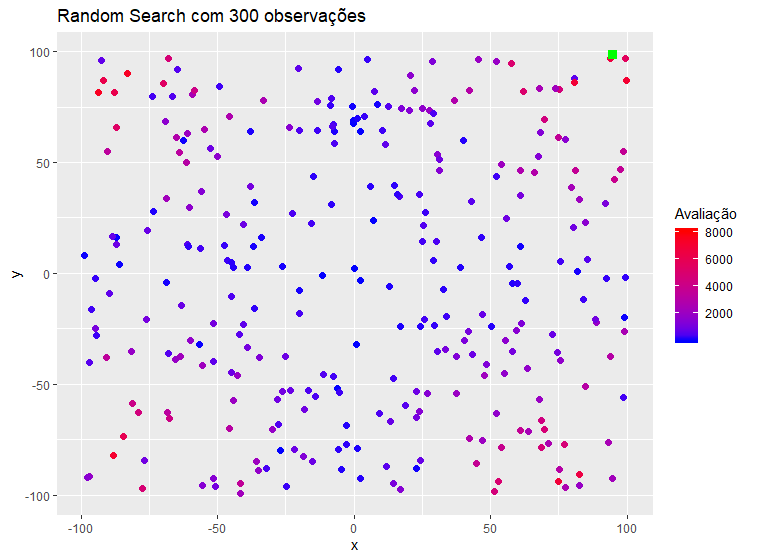
\includegraphics[width=0.8\linewidth]{imagens/scatter_rs_P30_T10.png}
%	\caption{Distribuição dos pontos na busca randômica (RS)}
%	\label{fig:scatter_RS}
%\end{figure}

\begin{figure}[ht]
	\centering
	\begin{subfigure}[b]{0.47\linewidth}
		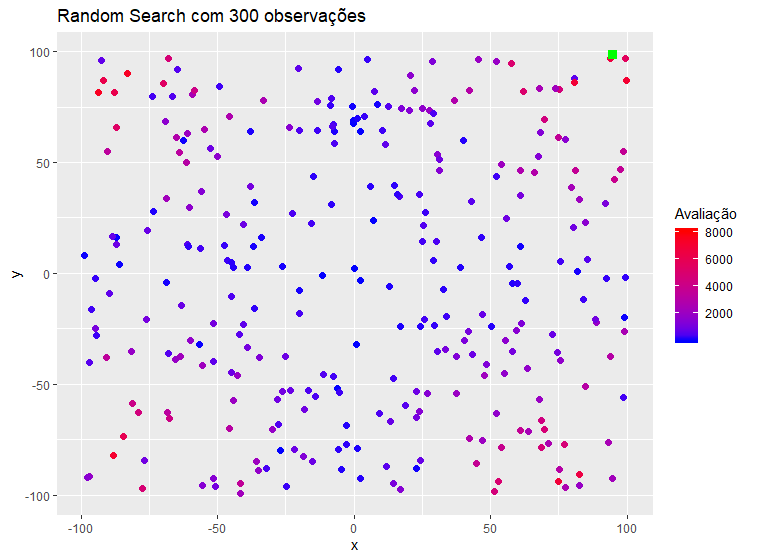
\includegraphics[width=\linewidth]{imagens/scatter_rs_P30_T10.png}
		\caption{Distribuição dos pontos gerados no RS}
	\end{subfigure}
	\begin{subfigure}[b]{0.47\linewidth}
		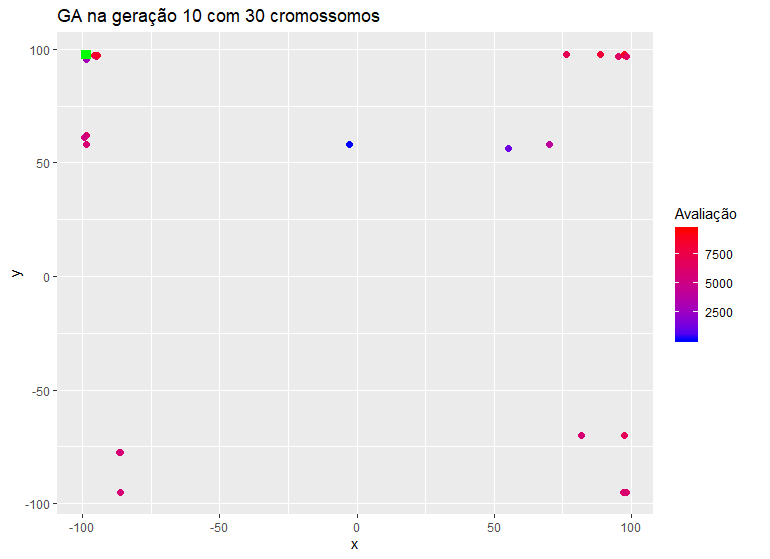
\includegraphics[width=\linewidth]{imagens/scatter_GA_P30_T10.png}
		\caption{Distribuição da ultima geração no GA}
	\end{subfigure}
	\begin{subfigure}[b]{0.65\linewidth}
		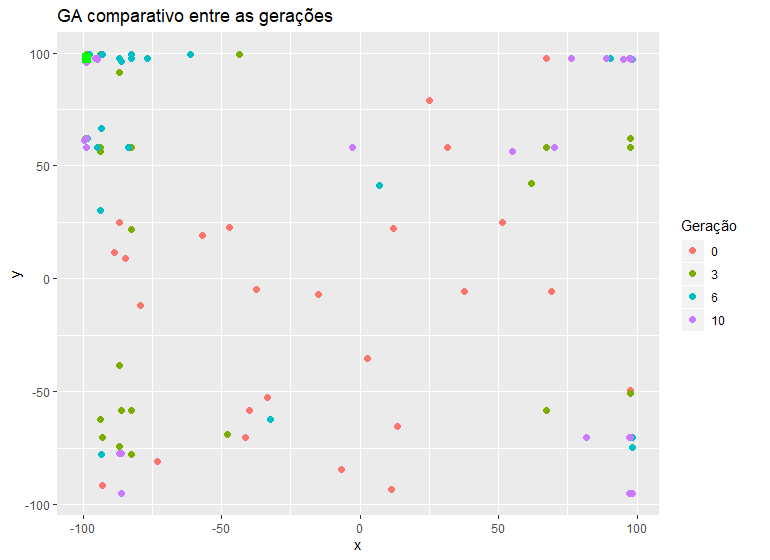
\includegraphics[width=\linewidth]{imagens/scatter_GA_P30_T10b.png}
		\caption{Comparativo entre algumas gerações do GA}
	\end{subfigure}
	\caption{Distribuições das soluções encontradas nos algoritmos de busca aleatória e GA}
	\label{fig:scatter_RS_GA}
\end{figure}



\section{Modelo de Ising}

O modelo de Ising\footnote{O modelo também é conhecido como Lenz-Ising, pois Lenz introduziu o modelo, porém nunca calculou nenhuma de suas propriedades} é um modelo da física para estudos de fênomenos magnéticos em materiais. Ising resolveu analiticamente o modelo para uma dimensão e depois Onsanger resolveu para uma rede quadrada (2D). Apesar do modelo ter sido elaborado para compreender melhor o propriedades magnéticas de certos materiais, ele se mostrou de grande utilidade para modelar problemas de outras áreas de estudos de fenômenos cooperativos, como por exemplo a dissertação de \citeonline{Lucena2014} onde usa o modelo de Ising aplicado a um estudo de criminalidade. É considerado um dos mais simples e estudado dos modelos de mecânica estatística.

O modelo define uma grade de \textit{spins} \(\sigma_s\) que podem conter os valores -1 e +1 somente. Esses spins possuem uma interação de energia dada por \(-J(s, s')\sigma_s\sigma_{s'}\), ou seja, o valor de energia de dois spins será \(-J(s, s')\) se os spins forem diferentes, e \(+J(s, s')\) se forem iguais, e adicionalmente podem interagir com um campo magnético externo \textit{h} com energia \(-h\sigma_s\). \cite{McCoy1973}.

Seja então \( \sigma_s \in \{ -1, +1 \} \) cada vértice do modelo, \(\Lambda\) representando a grade do modelo, e \(\Omega_{\Lambda} = \{-1, +1 \} ^ {\Lambda} \) o espaço de possíveis estados do modelo, define-se \(\sigma \in  \Omega_{\Lambda}\), \( \sigma = (\sigma_s)_{s \in \Lambda} \) como um estado possível do modelo de Ising para essas configurações. O Hamiltoniano do sistema para o estado \(\sigma\), \(\mathcal{H}(\sigma)\), será dado por: 

\[ \mathcal{H}(\sigma) = -\sum_{s,s' \in \Lambda}J(s,s')\sigma_{s}\sigma_{s'} -\sum_{s \in \Lambda}h \sigma_s \]

Sendo \(\beta = 1/\kappa \mathcal{T}\), com \(\mathcal{T}\) a temperatura em Kelvin e \(\kappa \) a constante de Boltzmann, a função de partição é definida por
\[ Z(\beta) = \sum_{\sigma \in \Omega_{\Lambda}} e^{-\beta \mathcal{H}(\sigma)} \]

e a probabilidade de encontrar o estado \(\sigma \)
\[ P(\sigma) = \frac{e^{-\beta \mathcal{H}(\sigma)}}{Z(\beta)} \]

Temperaturas altas deixam \(\beta\) baixo, o que torna a distribuição mais plana, e todos os estados tem probabilidades mais próximas de serem encontrados, conforme a temperatura baixa, os estados de menor energia passam a ter a maior probabilidade de ser encontrado.

O modelo de duas dimensões mais simples usa uma estrutura formada por quadrados com formato retangular de dimensões \(\Lambda = n \times m\), facilmente representada por uma matriz. Além disso \(J(s, s')\) é um valor fixo independente dos spins e que se \textit{s} e \textit{s'} não forem vizinhos será igual 0. Por fim será sem campo magnético externo, ou seja, \(h = 0\), e assim o Hamiltoniano pode ser reescrito na forma:

\begin{equation}
\mathcal{H}(\sigma) = - \sum_{i = 1}^{n-1} \sum_{j = 1}^{m-1} \Bigl( J(s,s')\sigma_{i,j}\sigma_{i,j+1} + J(s,s')\sigma_{i,j}\sigma_{i+1,j} \Bigr)
\label{eq:Energia_modelo_ising}
\end{equation}

O algoritmo genético simples será usado para apresentar uma solução, isto é \(\sigma\), para modelo de Ising em uma matriz \(10 \times 10\), com \(J(s,s') = 1\) para os spins vizinhos, sendo \(\Lambda = \left[1,10\right]^2\) as posições da matriz, e a função de avaliação utilizada será baseada na \autoref{eq:Energia_modelo_ising}.

\section{GA para o modelo de Ising}
A classe cromossomo será usada para representar cada solução para o problema e conterá um vetor de valores inteiros de tamanho $100$, representando assim a matriz \( 10 \times 10 \), alinhando uma linha da matriz na sequencia da outra no vetor. Assim o nosso genótipo é uma cadeia de inteiros, onde o fenótipo será a matriz correspondente quebrando o vetor em linhas de tamanho $10$.

Exemplo da relação genótipo x fenótipo para uma matriz \( 3 \times 3 \):
\begin{align*}
\text{cromossomo} &= \left[-1, 1, 1, 1, -1, 1, 1, 1, -1 \right]\\
\text{fenótipo} &= \begin{bmatrix}
-1 & 1 & 1 \\
1 & -1 & 1 \\
1 & 1 & -1
\end{bmatrix}
\end{align*}

Na implementação em Java, os cromossomos são definidos como classes, encapsulando os genes, os métodos dos operadores genéticos de crossover e mutação, e os métodos para avaliação e classificação dos cromossomos quando necessário. Para outros tipos de verificação cada cromossomo também guardou informações sobre seus cromossomos pais.

Para o método de seleção foi usado o método da roleta viciada, definindo a proporção de seleção de cada estado presente na população relacionado diretamente a sua função de avaliação. A primeira função testada foi usando o resultado da \autoref{eq:Energia_modelo_ising} somando o valor de \(\min\limits_{\sigma \in \Omega_{\sigma}}(\mathcal{H}(\sigma))\) e multiplicando por \(-1\) para conter somente valores positivos. Essa função não mostrou bons resultados pois não houve muita pressão seletiva, pois cromossomos com melhores valores recebiam pouco ou nenhum destaque na fase de seleção, assim o algoritmo precisava de muitas gerações para começar um avanço em encontrar melhores soluções. Na literatura sobre GA é mencionado o fato da função de avaliação ser muito plana o algoritmo passa a ser menos eficiente, isso também ocorre com outros métodos de otimização, como por exemplo os que usam gradientes por aproximação numérica, pois em funções que mostram pouco crescimento, a aproximação pode falhar em indicar a direção de maior crescimento. Os resultados para a seleção de uma das gerações pode ser visto na \autoref{tab:resumo_GA_H} do \refanexo{chap:anexos}. Para corrigir isso foi adotada a função de avaliação \(e^{-\beta \mathcal{H}(\sigma)} \) o que leva a uma probabilidade de seleção do indivíduo definida por:

\begin{equation}
Pr(\sigma) = \frac{e^{-\beta \mathcal{H}(\sigma)}}{\sum_{\sigma \in \theta_{\Lambda}}e^{-\beta \mathcal{H}(\sigma)}}
\label{eq:selecao_modelo_ising}
\end{equation}

Onde \(\theta_{\Lambda} \in \Omega_{\Lambda} \) representa a população de estados daquela geração do algoritmo e o método de seleção é parecido com o apresentado como seleção de Boltzmann na \autoref{subsec:selecao}. O problema que deve ser definido um novo parâmetro para o algoritmo dado por \(\beta \), que como valor inicial será usado o 0,05. Os resultados foram muito melhores e podem ser verificados na \autoref{tab:resumo_GA_expH} do \refanexo{chap:anexos}.

O operador de crossover será testado com o método de ponto único, dois pontos e uniforme, e para o operador de mutação cada posição do gene será sorteado com a probabilidade \(p_m\) para ser eleito para alteração e depois cada estado possível, no caso dois \(\{ -1, +1\}\), será sorteado com probabilidades iguais para definir o novo estado do gene.

A população inicial é definida sorteando os \(\sigma_s\) de cada posição das matrizes de cada um dos indivíduos. O programa terá definido uma classe para a população que é responsável por criar a geração inicial aleatória, controlar aspectos sobre a geração como melhor e pior cromossomo e algumas estatísticas sobre a população como quantidade de indivíduos que sofreram mutação e crossover, entre outros. 

Da mesma forma que o teste inicial, serão testados algumas variações dos parâmetros do algoritmo e comparado com os resultados da busca aleatória. Além disso será verificado, assim como no mencionado em \citeonline{Mitchell1996} sobre o trabalho de \citeonline{Pruegel-Bennett1994}, as distribuições dos valores de \(\mathcal{H}(\sigma)\) para as gerações 0, 10, 20, 30 e 40 do GA, e calculando as estatísticas para média e variância da amostra de 1000 testes. De forma ampliar as comparações dos resultados finais, os dois algoritmos foram modificado para ordenar as populações, que no caso do GA é feito a cada geração.

\section{Testes e resultados}
O começo da \autoref{tab:resultados_teste2} demonstra os resultados mantendo-se os parâmetros fixo e alterando apenas o método usado no crossover, indicado pelo índice nos valores de \(p_c\), com 1 para ponto único, 2 para crossover em dois pontos e \textit{u} para uniforme. Todos são muitos superiores ao método RS, provavelmente em virtude do espaço de soluções ser dado por \(2^{10*10}\) e a quantidade de observações geradas para o método cobrir uma parte pequena do espaço. 

\begin{table}[h!]
	\centering
	\begin{tabular}{|l|l|l|l|l|l|l|l|l|}
		\hline
		\multicolumn{4}{|c|}{\textbf{Parâmetros}}                                                    & \multicolumn{2}{c|}{\textbf{Resultados GA}}                                        & \multicolumn{2}{c|}{\textbf{Resultados RS}}                                        & \multicolumn{1}{c|}{\textbf{\#}}                      \\ \hline
		\textbf{\textit{n}} & \textbf{\textit{T}} & $\bm{p_c}$ & $\bm{p_m}$ & \textbf{Média $\pm$ IC} & \textbf{D.P.} & \textbf{Média $\pm$ IC} & \textbf{D.P.} & \textbf{GA < RS} \\ \hline
		30                          & 10                          & $0,8_1$    & 0,02       & -58.90 $\pm$ 0,54                            & 8,77                           & -39,05 $\pm$ 0,33                            & 5,43                           & 978                                          \\ \hline
		30                          & 10                          & $0,8_2$    & 0,02       & -60,21 $\pm$ 0,57                            & 9,33                           & -38,98 $\pm$ 0,32                            & 5,22                           & 970                                          \\ \hline
		30                          & 10                          & $0,8_u$    & 0,02       & -60,42 $\pm$ 0,63                            & 10,30                          & -39,39 $\pm$ 0,35                            & 5,68                           & 960                                          \\ \hline
		30                          & 100                         & $0,8_1$    & 0,02       & -122,24 $\pm$ 0,71                           & 11,57                          & -48,54 $\pm$ 0,27                            & 4,49                           & 1000                                         \\ \hline
		30                          & 100                         & $0,8_2$    & 0,02       & -126,05 $\pm$ 0,75                           & 12,19                          & -47,94 $\pm$ 0,27                            & 4,48                           & 1000                                         \\ \hline
		30                          & 100                         & $0,8_u$    & 0,02       & -130,47 $\pm$ 0,73                           & 11,89                          & -48,23 $\pm$ 0,28                            & 4,54                           & 1000                                         \\ \hline
	\end{tabular}
	\caption{Resultados da média de energia para 1000 testes com modelo Ising alterando tipo de crossover}
	\label{tab:resultados_teste2}
\end{table}

Comparando o resultado entre os 3 métodos de crossover, é possível pela média dos resultados verificar pequena melhora usando o método para 2 pontos e mais uma pequena melhora para o uniforme, mais visível nos testes com mais gerações. Isso pode ser explicado pela construção do genótipo do cromossomos, como cada linha da matriz está na sequência da outra, podemos ter \textit{clusters} com bom resultados de forma quadrada, como mostrado na \autoref{fig:Map_ising}. A região vermelha possui uma baixa energia contribuindo de forma positiva para a avaliação do indivíduo, porém essa área não consegue ser isolada pelos operadores de crossover de 1 ou 2 pontos, mas tem boa probabilidade de ser compartilhada em partes ou inteira através do operador uniforme. Outro fator que piora nessa condição é os genes caronistas, discutidos na \autoref{sec:problemas_GA}, pois a área azul ao apresentar pior resultado tem alta probabilidade de pegar carona com a área vermelha do cromossomo.

\begin{figure}[h!]
	\centering
	\includegraphics[width=0.35\linewidth]{imagens/Mapa_ising.png}
	\caption{Exemplo de uma região (vermelha) com baixa energia, próxima de outras com energias superiores}
	\label{fig:Map_ising}
\end{figure}



Nos próximos testes fica fixado o crossover uniforme, além disso pela característica do GA, quanto mais iterações do algoritmo permitida, melhores resultados deve apresentar, portanto serão avaliados os demais parâmetros e os resultados estão apresentados na \autoref{tab:resultados_teste3}. Pelos valores de média apresentado é possível ver que os parâmetros \(p_c = 0,8\) e \(p_m = 0,02\), apresentaram os melhores resultados, quando o \(p_m\) é aumentado, como o algoritmo não tem elitismo, é provável que os melhores esquemas se perdem com a mutação. O \(p_c\) com valores mais baixos teve um resultado pior, que indica que com menos crossover deve ter ocorrido menos \textit{exploitation} do algoritmo levando a uma convergência mais lenta.

\begin{table}[h!]
	\centering
	\begin{tabular}{|l|l|l|l|l|l|l|l|l|}
		\hline
		\multicolumn{4}{|c|}{\textbf{Parâmetros}}                                                    & \multicolumn{2}{c|}{\textbf{Resultados GA}}                                        & \multicolumn{2}{c|}{\textbf{Resultados RS}}                                        & \multicolumn{1}{c|}{\textbf{\#}}                      \\ \hline
		\textbf{\textit{n}} & \textbf{\textit{T}} & $\bm{p_c}$ & $\bm{p_m}$ & \textbf{Média $\pm$ IC} & \textbf{D.P.} & \textbf{Média $\pm$ IC} & \textbf{D.P.} & \textbf{GA < RS} \\ \hline
		30                          & 40                          & 0,8        & 0,02       & -105,07 $\pm$ 0,72                           & 11,66                          & -44,98 $\pm$ 0,31                            & 5,01                           & 1000                                      \\ \hline
		30                          & 40                          & 0,8        & 0,05       & -93,90 $\pm$ 0,71                            & 11,52                          & -44,63 $\pm$ 0,29                            & 4,81                           & 1000                                      \\ \hline
		30                          & 40                          & 0,8        & 0,01       & -101,69 $\pm$ 0,74                           & 11,96                          & -44,91 $\pm$ 0,30                            & 4,85                           & 1000                                      \\ \hline
		40                          & 40                          & 0,8        & 0,02       & -111,06 $\pm$ 0,73                           & 11,89                          & -46,24 $\pm$ 0,30                            & 4,87                           & 1000                                      \\ \hline
		40                          & 40                          & 0,8        & 0,01       & -109,59 $\pm$ 0,73                           & 11,84                          & -46,02 $\pm$ 0,31                            & 5,04                           & 1000                                      \\ \hline
		30                          & 40                          & 0,95       & 0,02       & -108,42 $\pm$ 0,75                           & 12,15                          & -44,91 $\pm$ 0,31                            & 5,14                           & 1000                                      \\ \hline
		30                          & 40                          & 0,7        & 0,02       & -101,26 $\pm$ 0,69                           & 11,27                          & -44,78 $\pm$ 0,31                            & 5,10                           & 1000                                      \\ \hline
	\end{tabular}
	\caption{Resultados da média de energia para 1000 testes com modelo Ising alterando outros parâmetros}
	\label{tab:resultados_teste3}
\end{table}

Os resultados mostrados foram para o melhor cromossomo encontrado entre todas as gerações do GA. A \autoref{tab:resultados_teste4} mostra mais dois resultados para a implementação do elitismo mantendo os 3 melhores cromossomos para a próxima população. Os valores indicam que houve pequena melhora no algoritmo.

\begin{table}[h!]
	\centering
	\begin{tabular}{|l|l|l|l|l|l|l|l|l|}
		\hline
		\multicolumn{4}{|c|}{\textbf{Parâmetros}}                                                    & \multicolumn{2}{c|}{\textbf{Resultados GA}}                                        & \multicolumn{2}{c|}{\textbf{Resultados RS}}                                        & \multicolumn{1}{c|}{\textbf{\#}}                      \\ \hline
		\textbf{\textit{n}} & \textbf{\textit{T}} & $\bm{p_c}$ & $\bm{p_m}$ & \textbf{Média $\pm$ IC} & \textbf{D.P.} & \textbf{Média $\pm$ IC} & \textbf{D.P.} & \textbf{GA < RS} \\ \hline
		30                          & 40                          & 0,8        & 0,02       & -110,66 $\pm$ 0,66                           & 10,73                          & -44,81 $\pm$ 0,30                            & 5,88                           & 1000                                      \\ \hline
		30                          & 40                          & 0,95        & 0,02       & -113,69 $\pm$ 0,70                            & 11,36                          & -44,75 $\pm$ 0,30                            & 4,99                           & 1000                                      \\ \hline
	\end{tabular}
	\caption{Resultados da média de energia para 1000 testes com modelo Ising e usando elitismo mantendo 3 cromossomos}
	\label{tab:resultados_teste4}
\end{table}

Outro parâmetro que pode ser modificado é \(\beta\), introduzido na função de avaliação e portanto com impacto direto na seleção. A \autoref{tab:resultados_teste5} mostra os resultados que se comportam como o esperado. Diminuir o \(\beta\) equivale aumentar a temperatura, e todos os estados passam a ter maior probabilidade de ser selecionado. Já quando o valor é elevado, ou seja, a temperatura fica menor, os estados de menor energia possuem maior probabilidade de ocorrerem, o que eleva a pressão seletiva do algoritmo. 

\begin{table}[h!]
	\centering
	\begin{tabular}{|l|l|l|l|l|l|l|l|l|l|}
		\hline
		\multicolumn{5}{|c|}{\textbf{Parâmetros}}                                                    & \multicolumn{2}{c|}{\textbf{Resultados GA}}                                        & \multicolumn{2}{c|}{\textbf{Resultados RS}}                                        & \multicolumn{1}{c|}{\textbf{\#}}                      \\ \hline
		\textbf{\textit{n}} & \textbf{\textit{T}} & $\bm{p_c}$ & $\bm{p_m}$ & $\beta$ & \textbf{Média $\pm$ IC} & \textbf{D.P.} & \textbf{Média $\pm$ IC} & \textbf{D.P.} & \textbf{GA < RS} \\ \hline
		30                          & 40                          & 0,8        & 0,02  & 0,05      & -113,69 $\pm$ 0,70                           & 11,36                          & -44,75 $\pm$ 0,30                            & 4,99                           & 1000                                      \\ \hline
		30                          & 40                          & 0,95        & 0,02 & 0,01      & -90,78 $\pm$ 0,66                            & 10,74                          & -44,79 $\pm$ 0,30                            & 4,87                           & 1000                                      \\ \hline
		30                          & 40                          & 0,95        & 0,02 & 0,1      & -120,45 $\pm$ 0,70                            & 11,35                          & -44,95 $\pm$ 0,30                            & 4,95                           & 1000                                      \\ \hline
	\end{tabular}
	\caption{Resultados da média de energia para 1000 testes com modelo Ising, usando elitismo com 3 cromossomos e variando \(\beta\)}
	\label{tab:resultados_teste5}
\end{table}

\begin{figure}[h!]
	\centering
	\begin{subfigure}[b]{0.47\linewidth}
		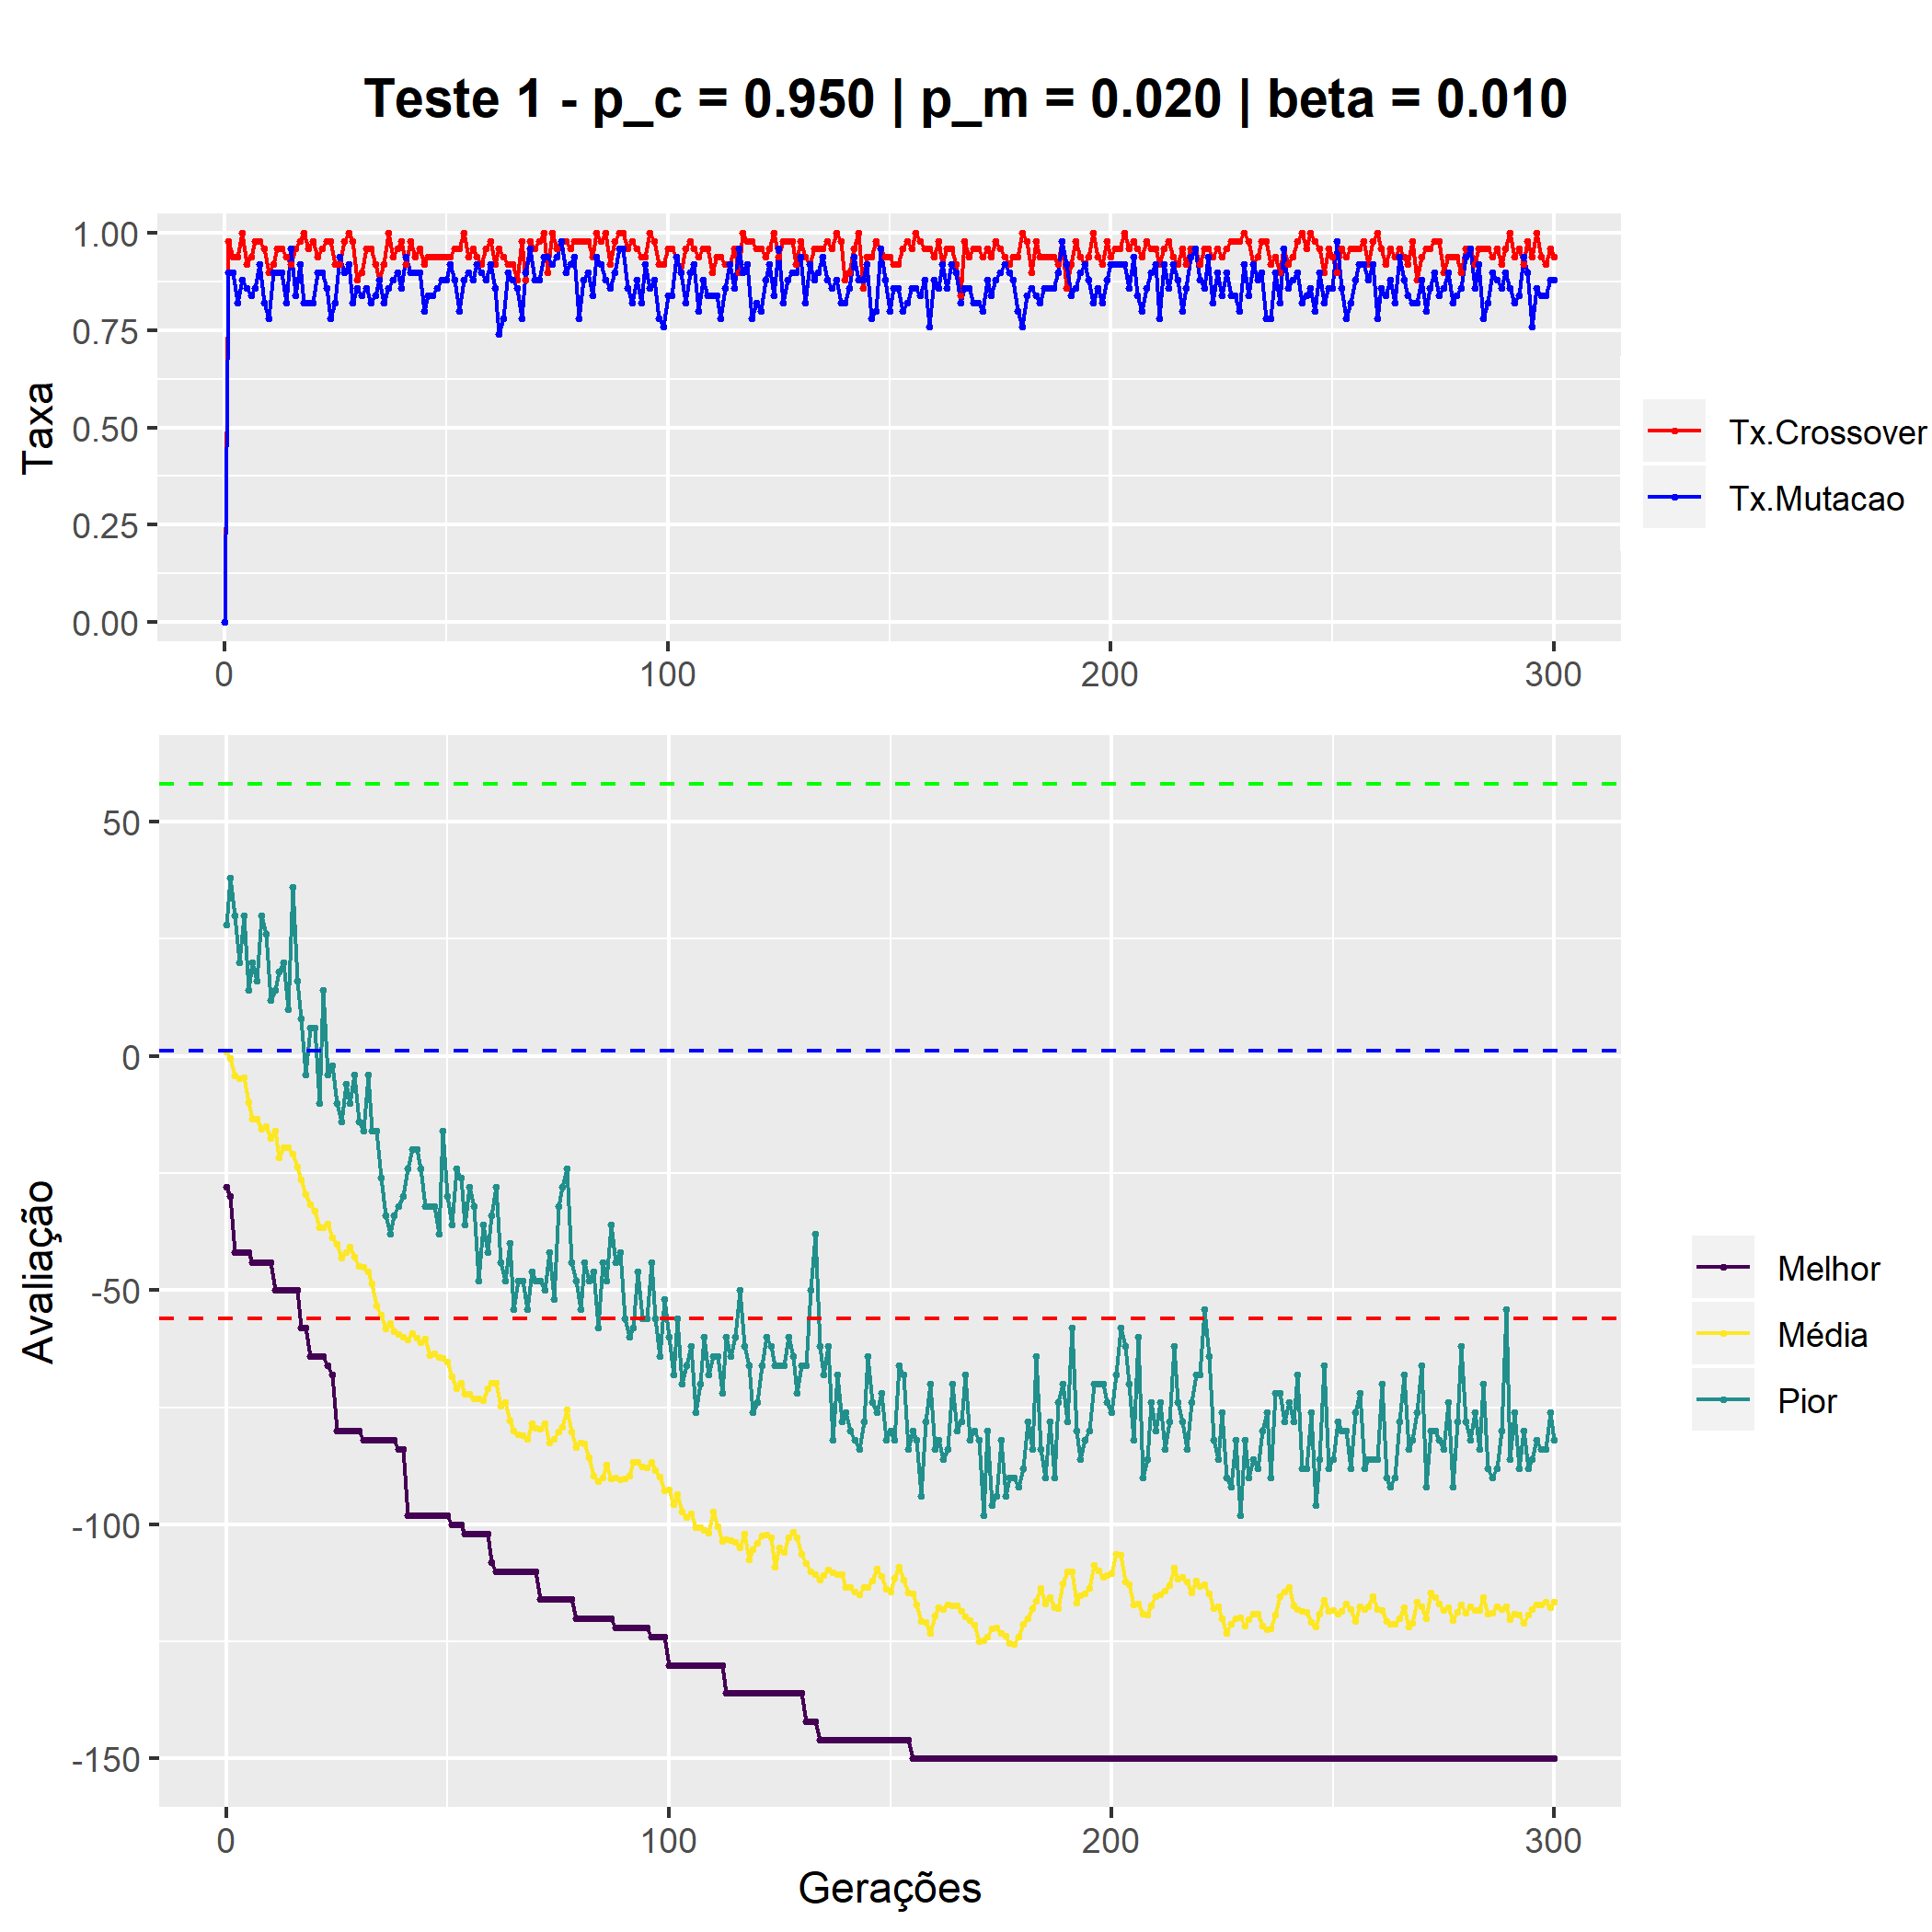
\includegraphics[width=\linewidth]{imagens/graph_pc_0_950_pm_0_020_pop_50_g_300__1_beta_0_01.png}
		\caption{}
	\end{subfigure}
	\begin{subfigure}[b]{0.47\linewidth}
		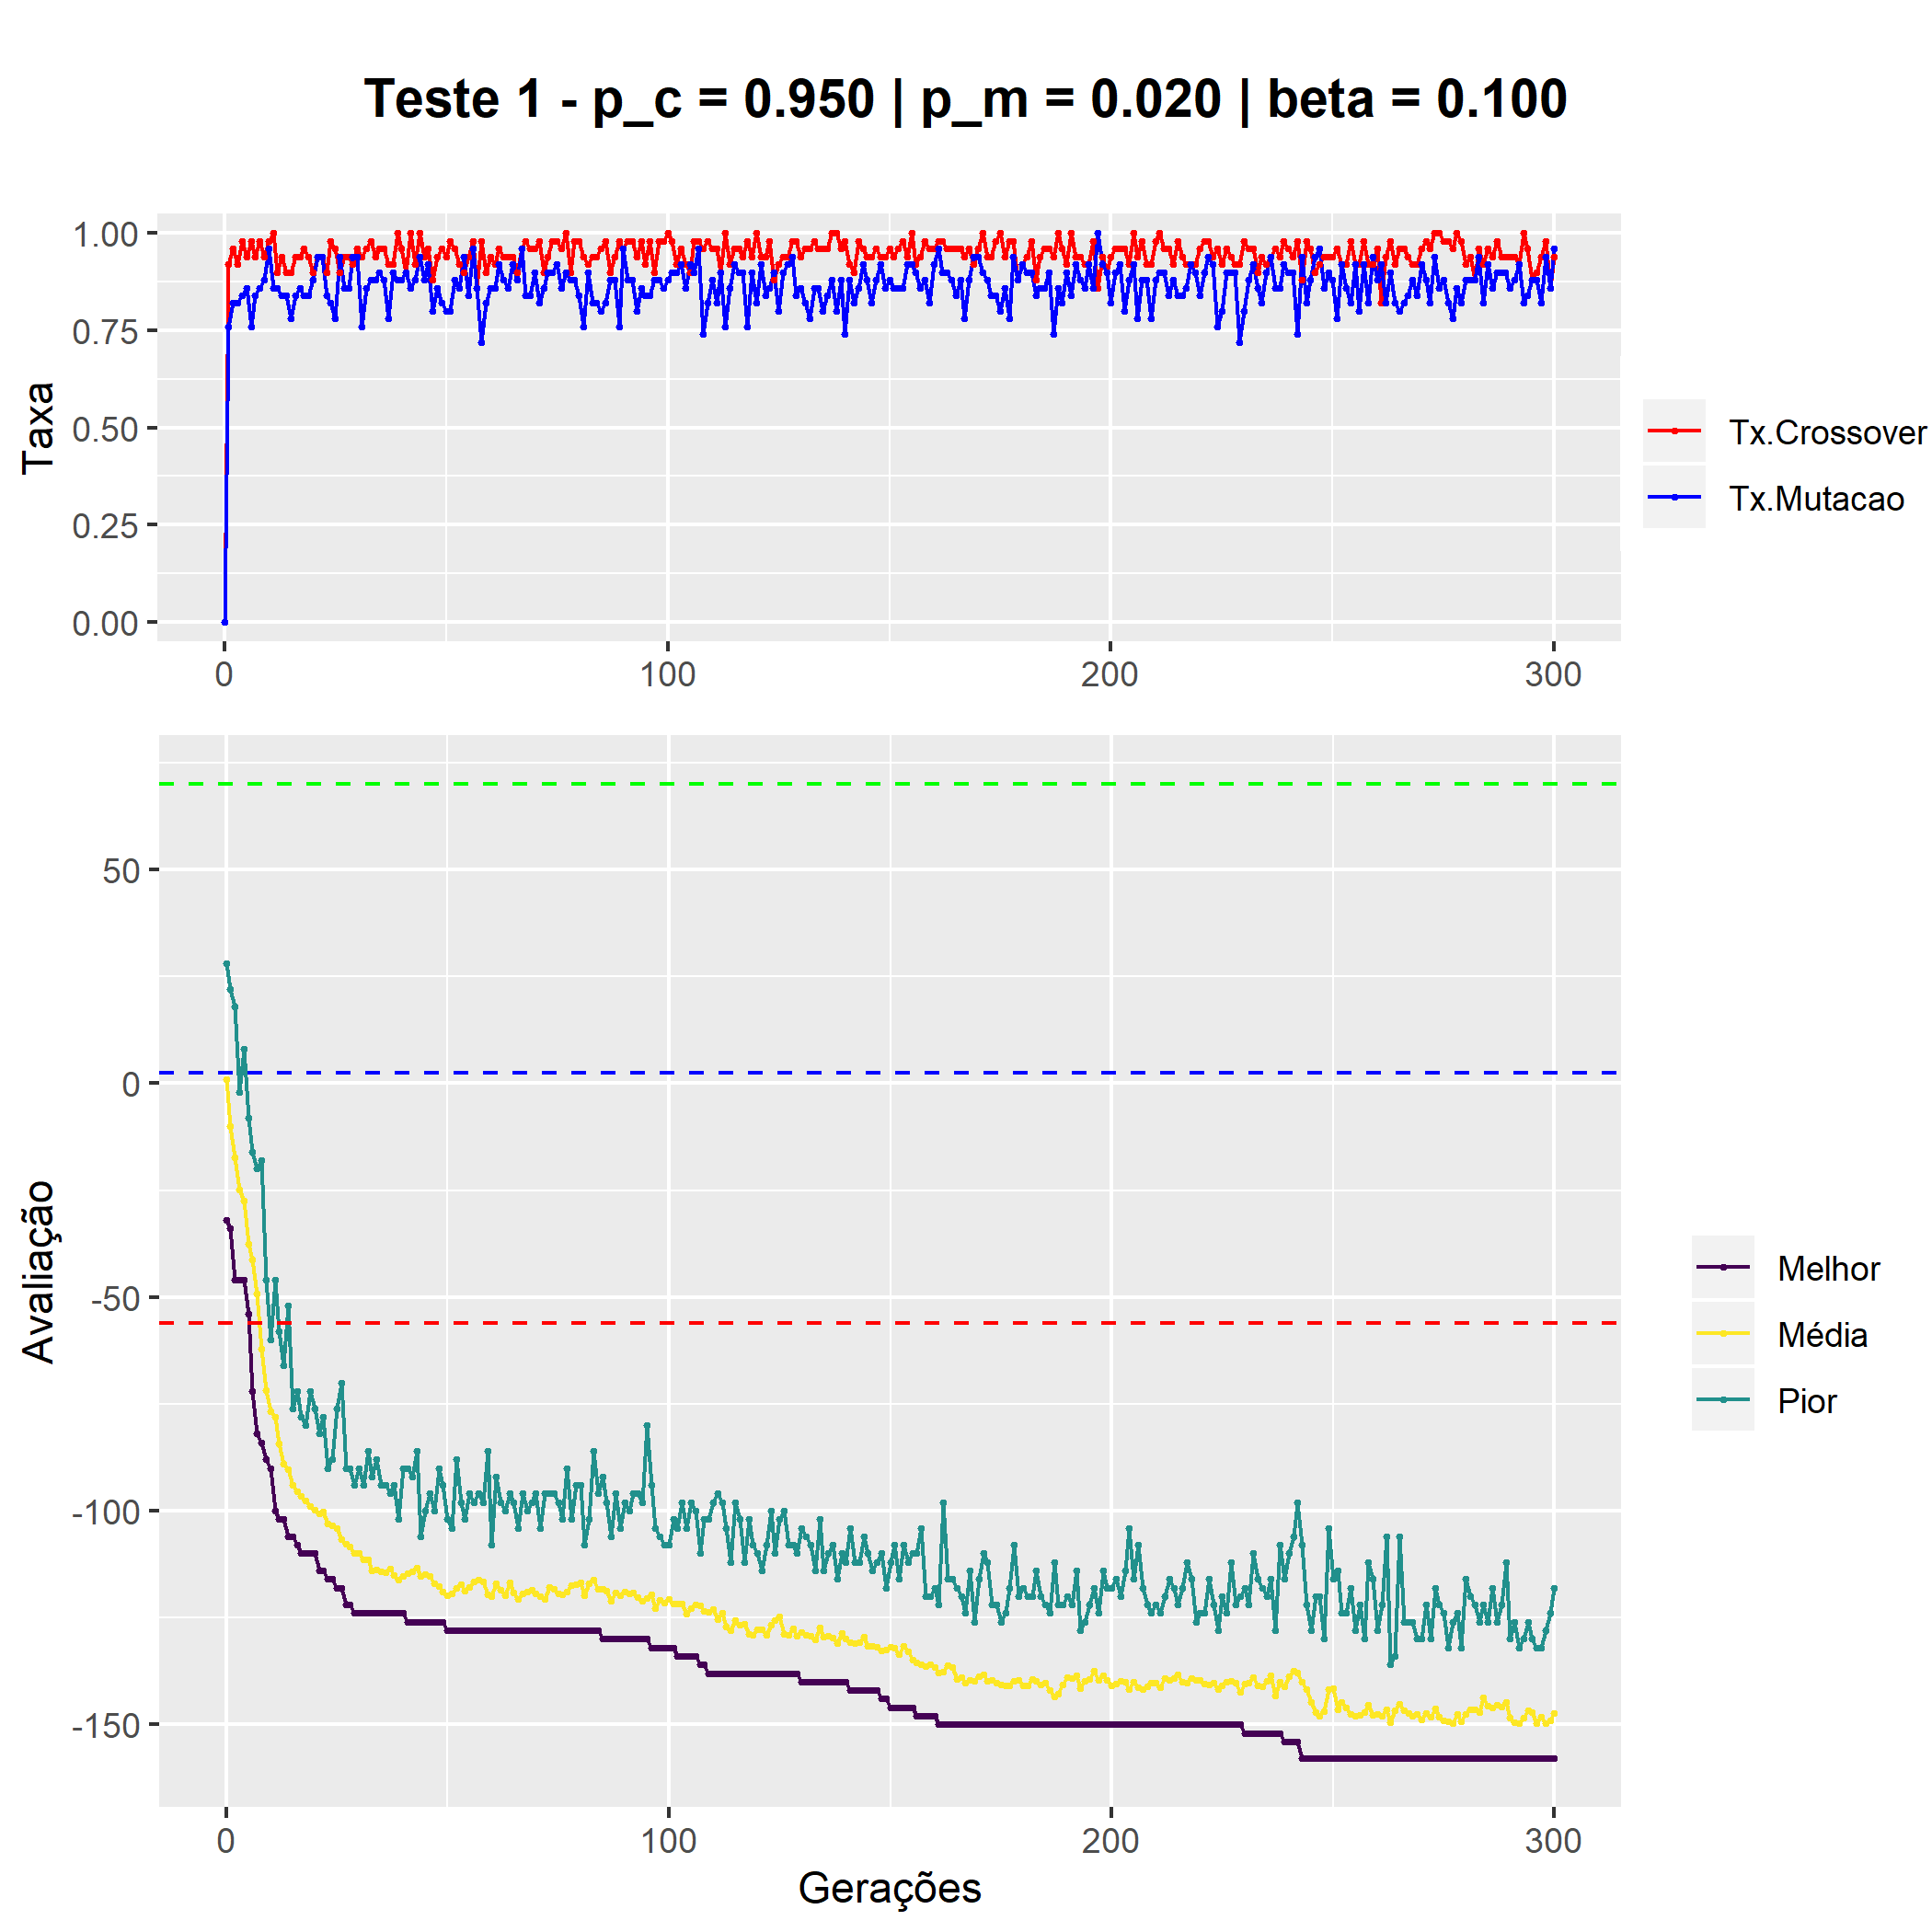
\includegraphics[width=\linewidth]{imagens/graph_pc_0_950_pm_0_020_pop_50_g_300__1_beta_0_1.png}
		\caption{}
	\end{subfigure}
	\begin{subfigure}[b]{0.47\linewidth}
		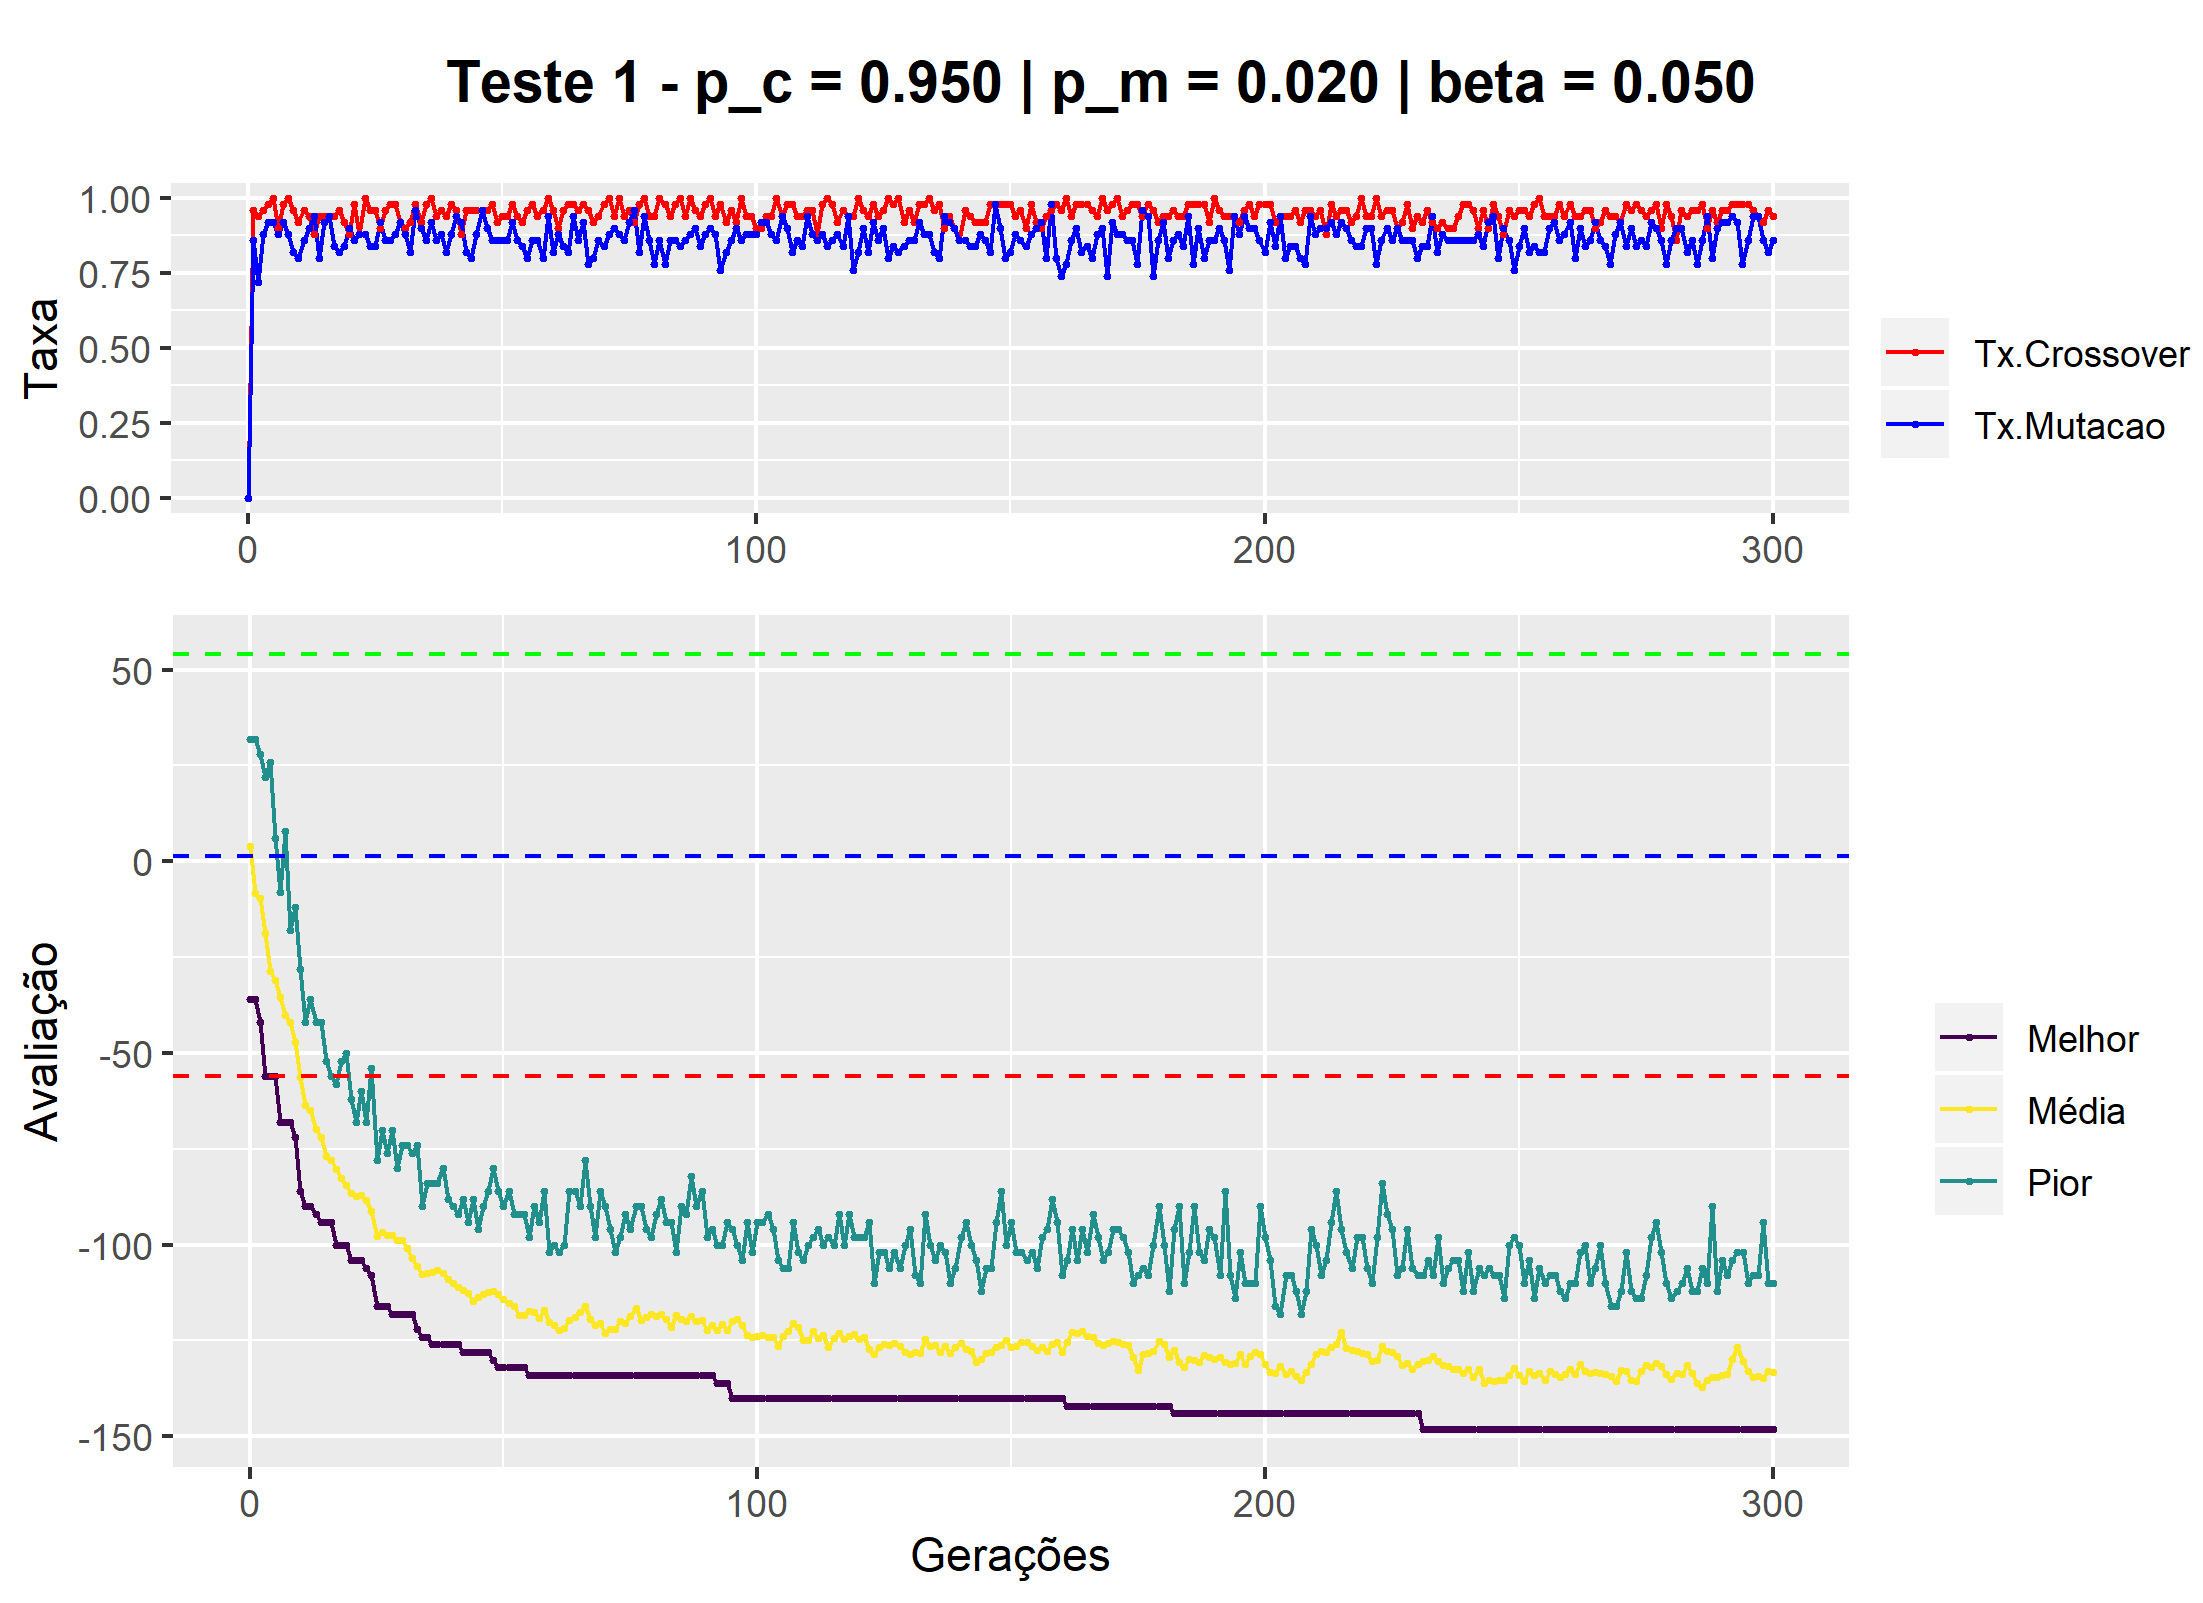
\includegraphics[width=\linewidth]{imagens/graph_pc_0_950_pm_0_020_pop_50_g_300__1_beta_0_05.png}
		\caption{}
	\end{subfigure}
	\begin{subfigure}[b]{0.47\linewidth}
		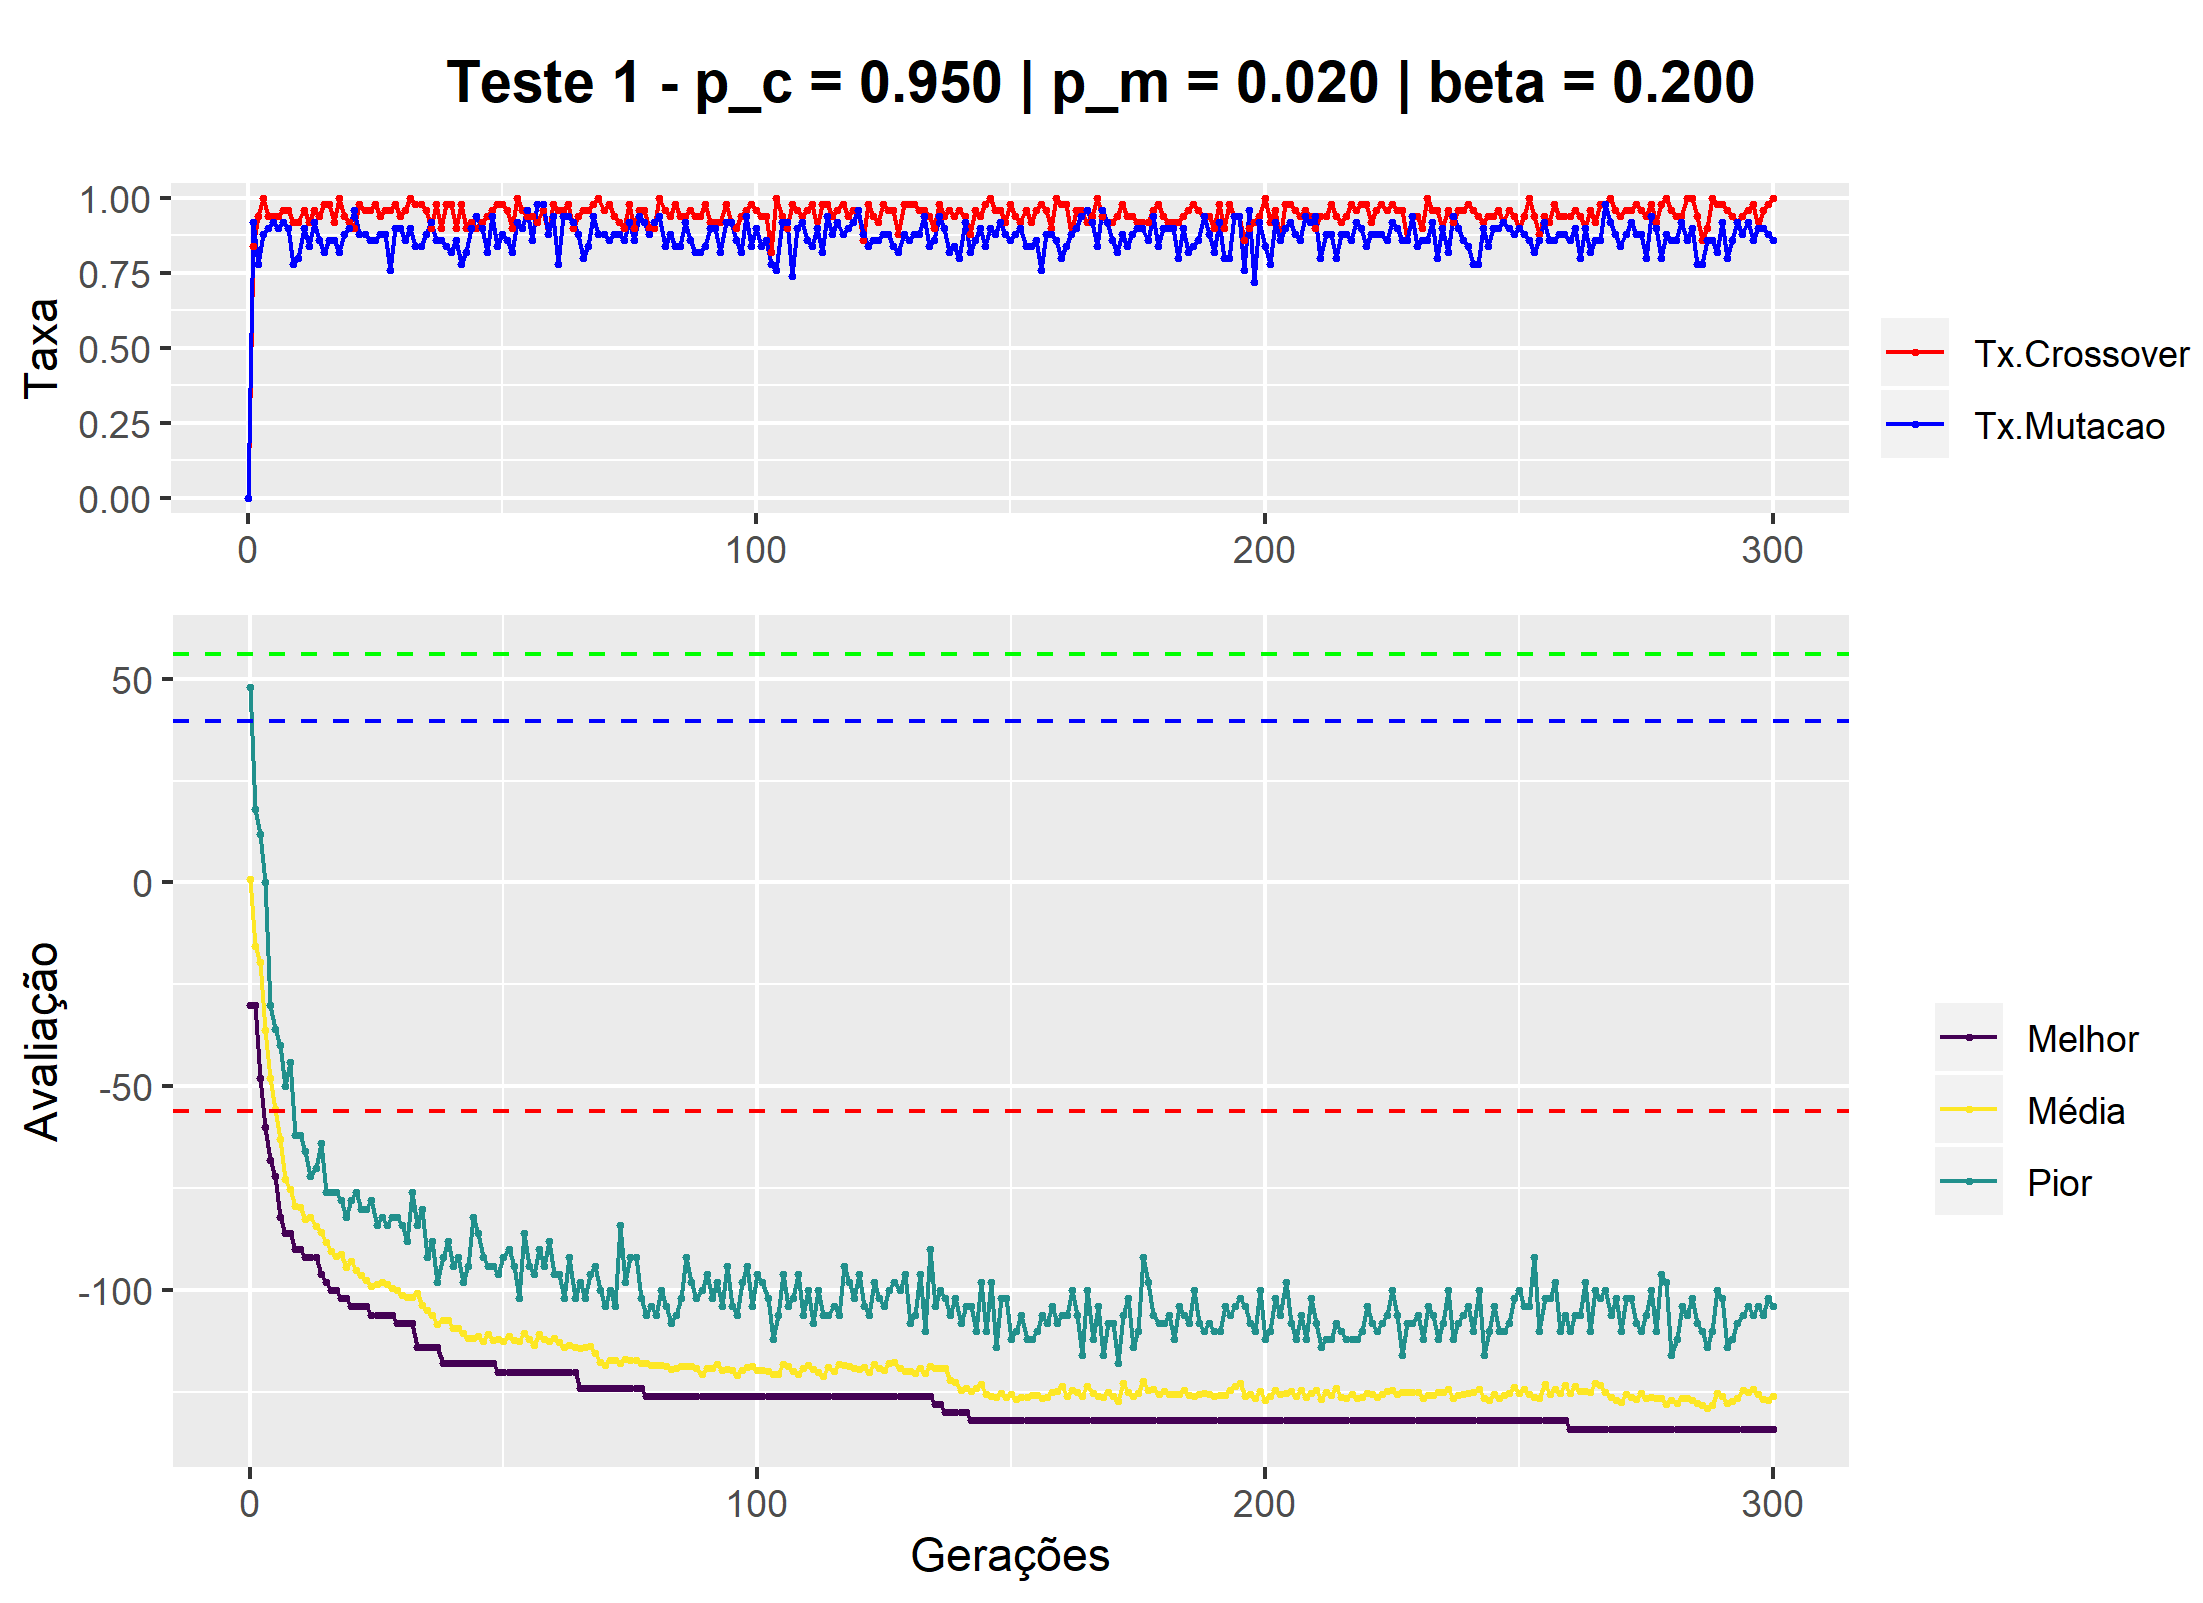
\includegraphics[width=\linewidth]{imagens/graph_pc_0_950_pm_0_020_pop_50_g_300__1_beta_0_2.png}
		\caption{}
	\end{subfigure}
	\caption{Evolução do GA variando o \(\beta\)}
	\label{fig:evolucaoGA_beta}
\end{figure}

Na \autoref{fig:evolucaoGA_beta} percebe-se que ao aumentar o \(\beta\), o algoritmo converge mais rapidamente e pode gerar melhores soluções, porém é necessário manter o equilíbrio entre o \textit{exploitation} e \textit{exploration}. Um valor muito alto para esse parâmetro, pode levar a uma convergência genética prematura, diminuindo as possibilidades de exploração do espaço de soluções (\textit{exploration}).

Para completar as avaliações, mantendo os parâmetros \(n = 50\), \(T = 40\), \(p_c = 0,95\), \(p_m = 0,02\) e com elitismo mantendo 3 cromossomos, foram salvos os valores de energia da população dos 1000 testes para as gerações 0, 10, 20, 30 e 40. Depois foi calculado a média e variância dessas gerações para cada um dos testes e finalmente feita a média dos parâmetros entre os 1000 testes obtendo os valores mostrados na \autoref{tab:resultados_medias_var}

\begin{table}[h!]
	\centering
	\begin{tabular}{|l|c|c|c|c|c|}
		\hline
		\textbf{Geração}   & \textbf{0} & \textbf{10} & \textbf{20} & \textbf{30} & \textbf{40} \\ \hline
		\textbf{Média}     & 0,00       & -47,49      & -78,76      & -96,46      & -106,86      \\ \hline
		\textbf{Variância} & 178,55     & 158,42      & 117,09       & 106,79       & 103,55       \\ \hline
	\end{tabular}
	\caption{Resultados da média de energia para 1000 testes das gerações 0, 10, 20, 30 e 40 do modelo Ising e usando elitismo com 3 cromossomos}
	\label{tab:resultados_medias_var}
\end{table}

\begin{figure}[h!]
	\centering
	\begin{subfigure}[b]{0.47\linewidth}
		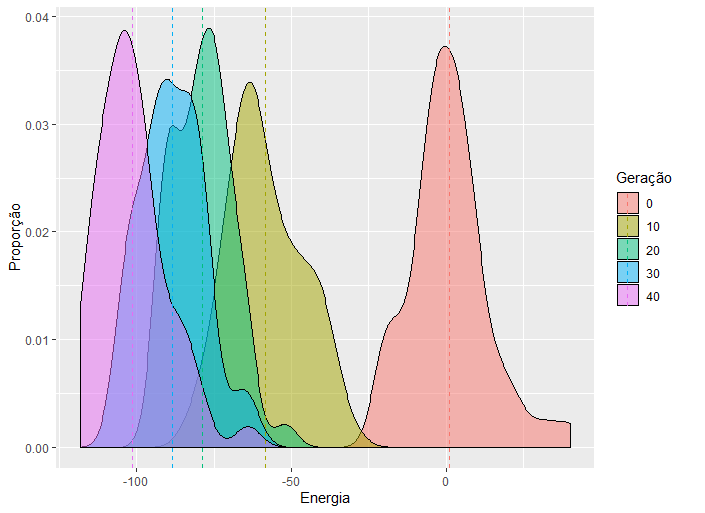
\includegraphics[width=\linewidth]{imagens/distribuicao_t50.png}
		\caption{Distribuição das amostras no teste 50}
	\end{subfigure}
	\begin{subfigure}[b]{0.47\linewidth}
		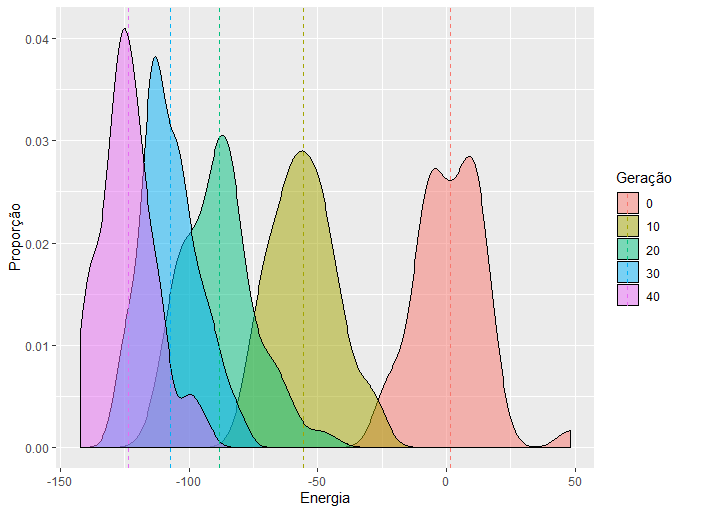
\includegraphics[width=\linewidth]{imagens/distribuicao_t491.png}
		\caption{Distribuição das amostras no teste 491}
	\end{subfigure}
	\begin{subfigure}[b]{0.47\linewidth}
		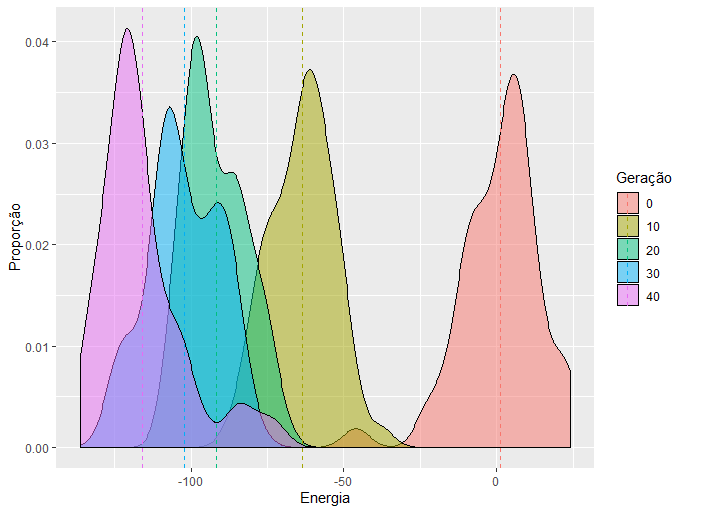
\includegraphics[width=\linewidth]{imagens/distribuicao_t900.png}
		\caption{Distribuição das amostras no teste 900}
	\end{subfigure}
	\begin{subfigure}[b]{0.47\linewidth}
		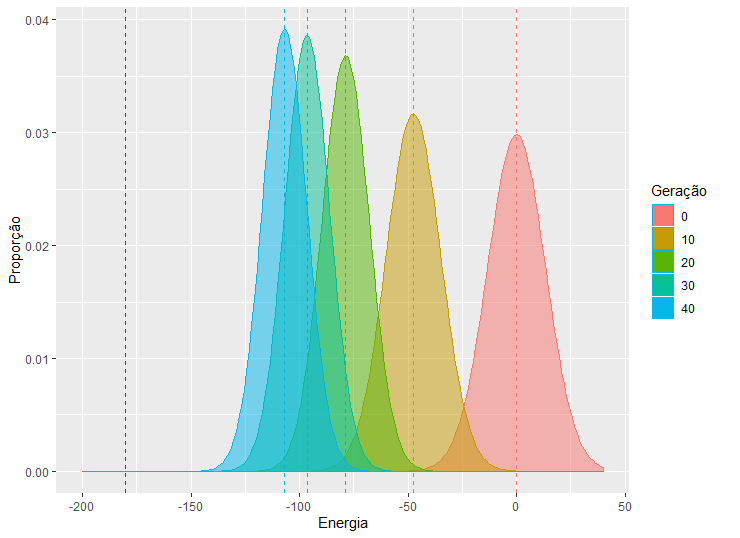
\includegraphics[width=\linewidth]{imagens/Distribuicao_medias.png}
		\caption{Usando média dos valores e considerando distribuição normal}
	\end{subfigure}
	\caption{Distribuições das populações para gerações 0, 10, 20 e 40, com \(p_m=0,02\)}
	\label{fig:distribuicao_ising_1}
\end{figure}

Diferente dos resultados vistos em \citeonline{Pruegel-Bennett1994}, que não usou operador de mutação, a variância no teste executado reduz pouco conforme se passam as gerações, o que é esperado já que a mutação busca manter diversidade na população. Refazendo os testes com \(p_m = 0\) obtemos a seguinte \autoref{tab:resultados_medias_var2}. O operador de mutação mantém a variância na população pois ele garante o \textit{exploration}, mantendo a diversidade da população.

\begin{table}[h!]
	\centering
	\begin{tabular}{|l|c|c|c|c|c|}
		\hline
		\textbf{Geração}   & \textbf{0} & \textbf{10} & \textbf{20} & \textbf{30} & \textbf{40} \\ \hline
		\textbf{Média}     & -0,02       & -52,34      & -85,29      & -96,25      & -98,72      \\ \hline
		\textbf{Variância} & 180,96     & 120,07      & 36,62       & 8,01       & 1,54       \\ \hline
	\end{tabular}
	\caption{Resultados da média de energia para 1000 testes com modelo Ising usando elitismo mantendo 3 cromossomos}
	\label{tab:resultados_medias_var2}
\end{table}


\begin{figure}[h!]
	\centering
	\begin{subfigure}[b]{0.47\linewidth}
		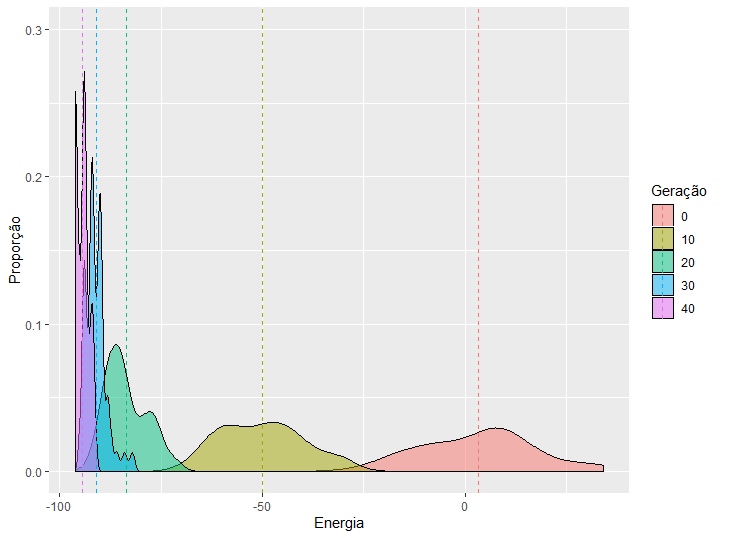
\includegraphics[width=\linewidth]{imagens/distribuicao_t43_2.png}
		\caption{Distribuição das amostras no teste 43}
	\end{subfigure}
	\begin{subfigure}[b]{0.47\linewidth}
		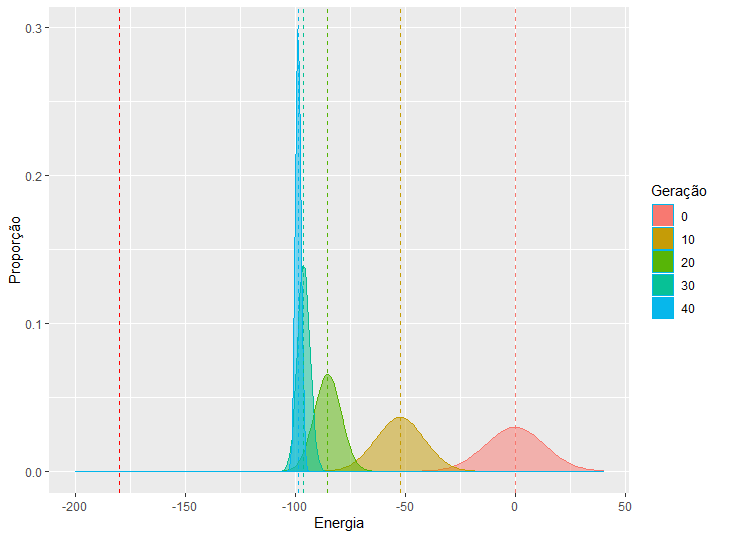
\includegraphics[width=\linewidth]{imagens/Distribuicao_medias2.png}
		\caption{Usando média dos valores e considerando distribuição normal}
	\end{subfigure}
	\begin{subfigure}[b]{0.67\linewidth}
		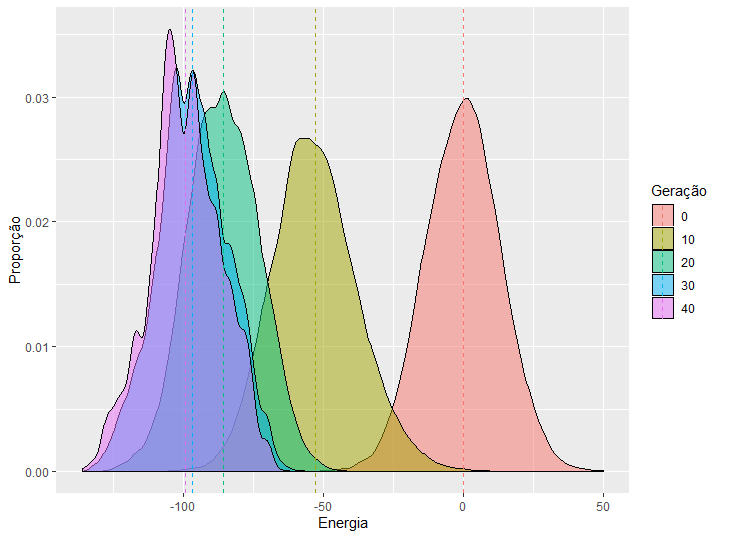
\includegraphics[width=\linewidth]{imagens/Distribuicao_amostral_500_testes_sem_mut.png}
		\caption{Usando amostra dos 500 testes e agrupando por geração}
	\end{subfigure}
\caption{Distribuições das populações para gerações 0, 10, 20 e 40, com \(p_m=0,\)}
	\label{fig:distribuicao_ising_2}
\end{figure}

Na \autoref{fig:distribuicao_ising_geracoes} pode ser visto os resultados das médias e variâncias da população durante as gerações. Os gráficos representam a média das duas medidas de cada geração pelos 500 testes realizados. Quando a taxa de mutação é mantida em 0, percebe-se a rápida convergência do GA, chegando a um patamar mínimo de energia, e a variância com tendência a zero. Ao colocar uma pequena taxa de mutação, o algoritmo converge mais lentamente, porém obtém resultados de média melhores, e a variância se mantém em um patamar. Isso é desejável no GA, pois indica que se manteve a diversidade genética. Além disso também é mostrado novamente o desempenho entre os operadores de crossover de um ponto e uniforme, e como esperado, o uniforme conseguiu médias melhores, mas a variância levou mais iterações para diminuir, justificado pelo fato desse operador obter maior diversidade genética no início, explorando melhor o espaço de soluções e garantindo melhores médias.

\begin{figure}[h!]
	\centering
	\begin{subfigure}[b]{0.47\linewidth}
		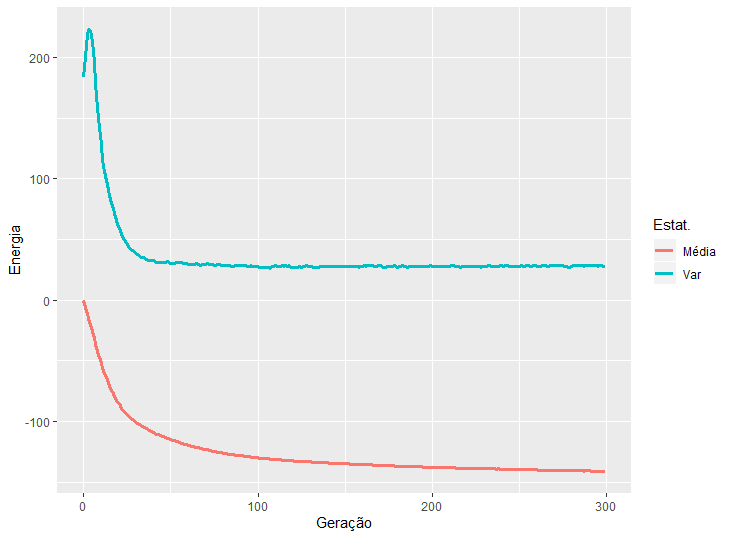
\includegraphics[width=\linewidth]{imagens/curva_media_var_1.png}
		\caption{Usando \(p_m = 0,005\)}
	\end{subfigure}
	\begin{subfigure}[b]{0.47\linewidth}
		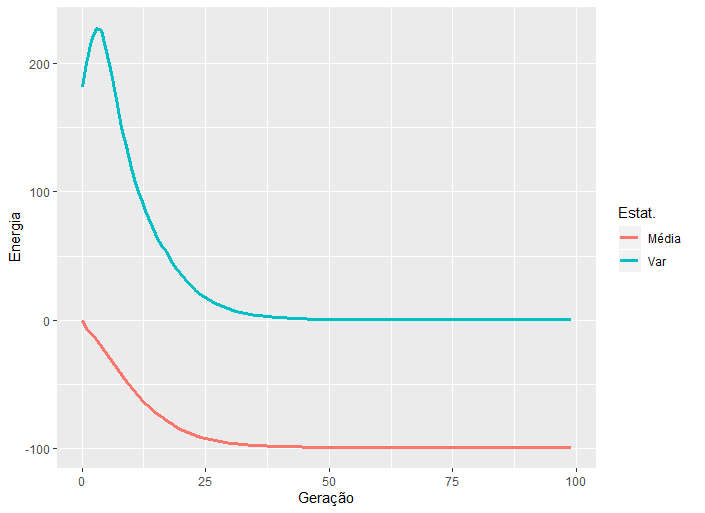
\includegraphics[width=\linewidth]{imagens/curva_media_var_2.png}
		\caption{Usando \(p_m = 0\)}
	\end{subfigure}
	\begin{subfigure}[b]{0.67\linewidth}
		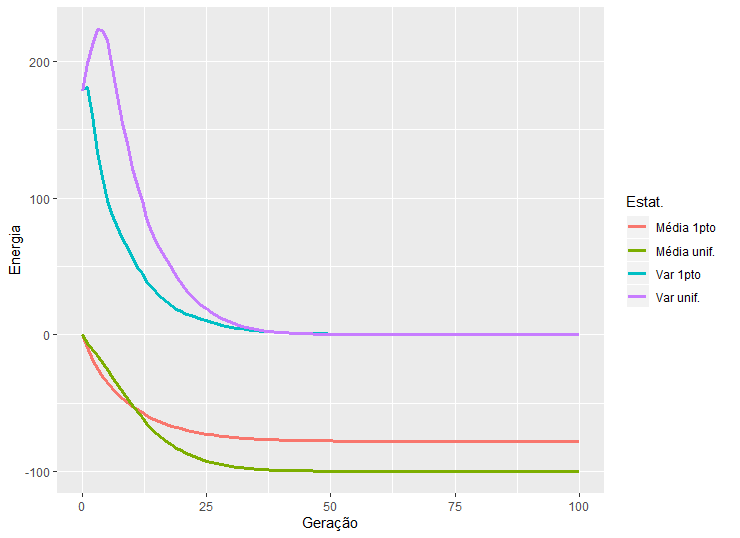
\includegraphics[width=\linewidth]{imagens/comp_cross_1pto_unif.png}
		\caption{Usando \(p_m = 0\) e comparando dois métodos de crossover}
	\end{subfigure}
\caption{Valores das médias e variâncias da população durante as gerações com \(p_m=0,005\). Os valores apresentados são da média de 500 testes}
	\label{fig:distribuicao_ising_geracoes}
\end{figure}

Por último na \autoref{fig:evolucaoGA} é exposto a evolução do algoritmo durante as gerações com variações no parâmetro de probabilidade de mutação, mostrando o melhor, pior cromossomo da população além de sua avaliação média. As linhas horizontais tracejadas mostram o melhor, pior e média do método de busca aleatório, considerando sempre a amostra para esse método de tamanho \(n \cdot T\) e portanto com \(50 \cdot 300 = 15000\) observações.

\begin{figure}[h!]
	\centering
	\begin{subfigure}[b]{0.47\linewidth}
		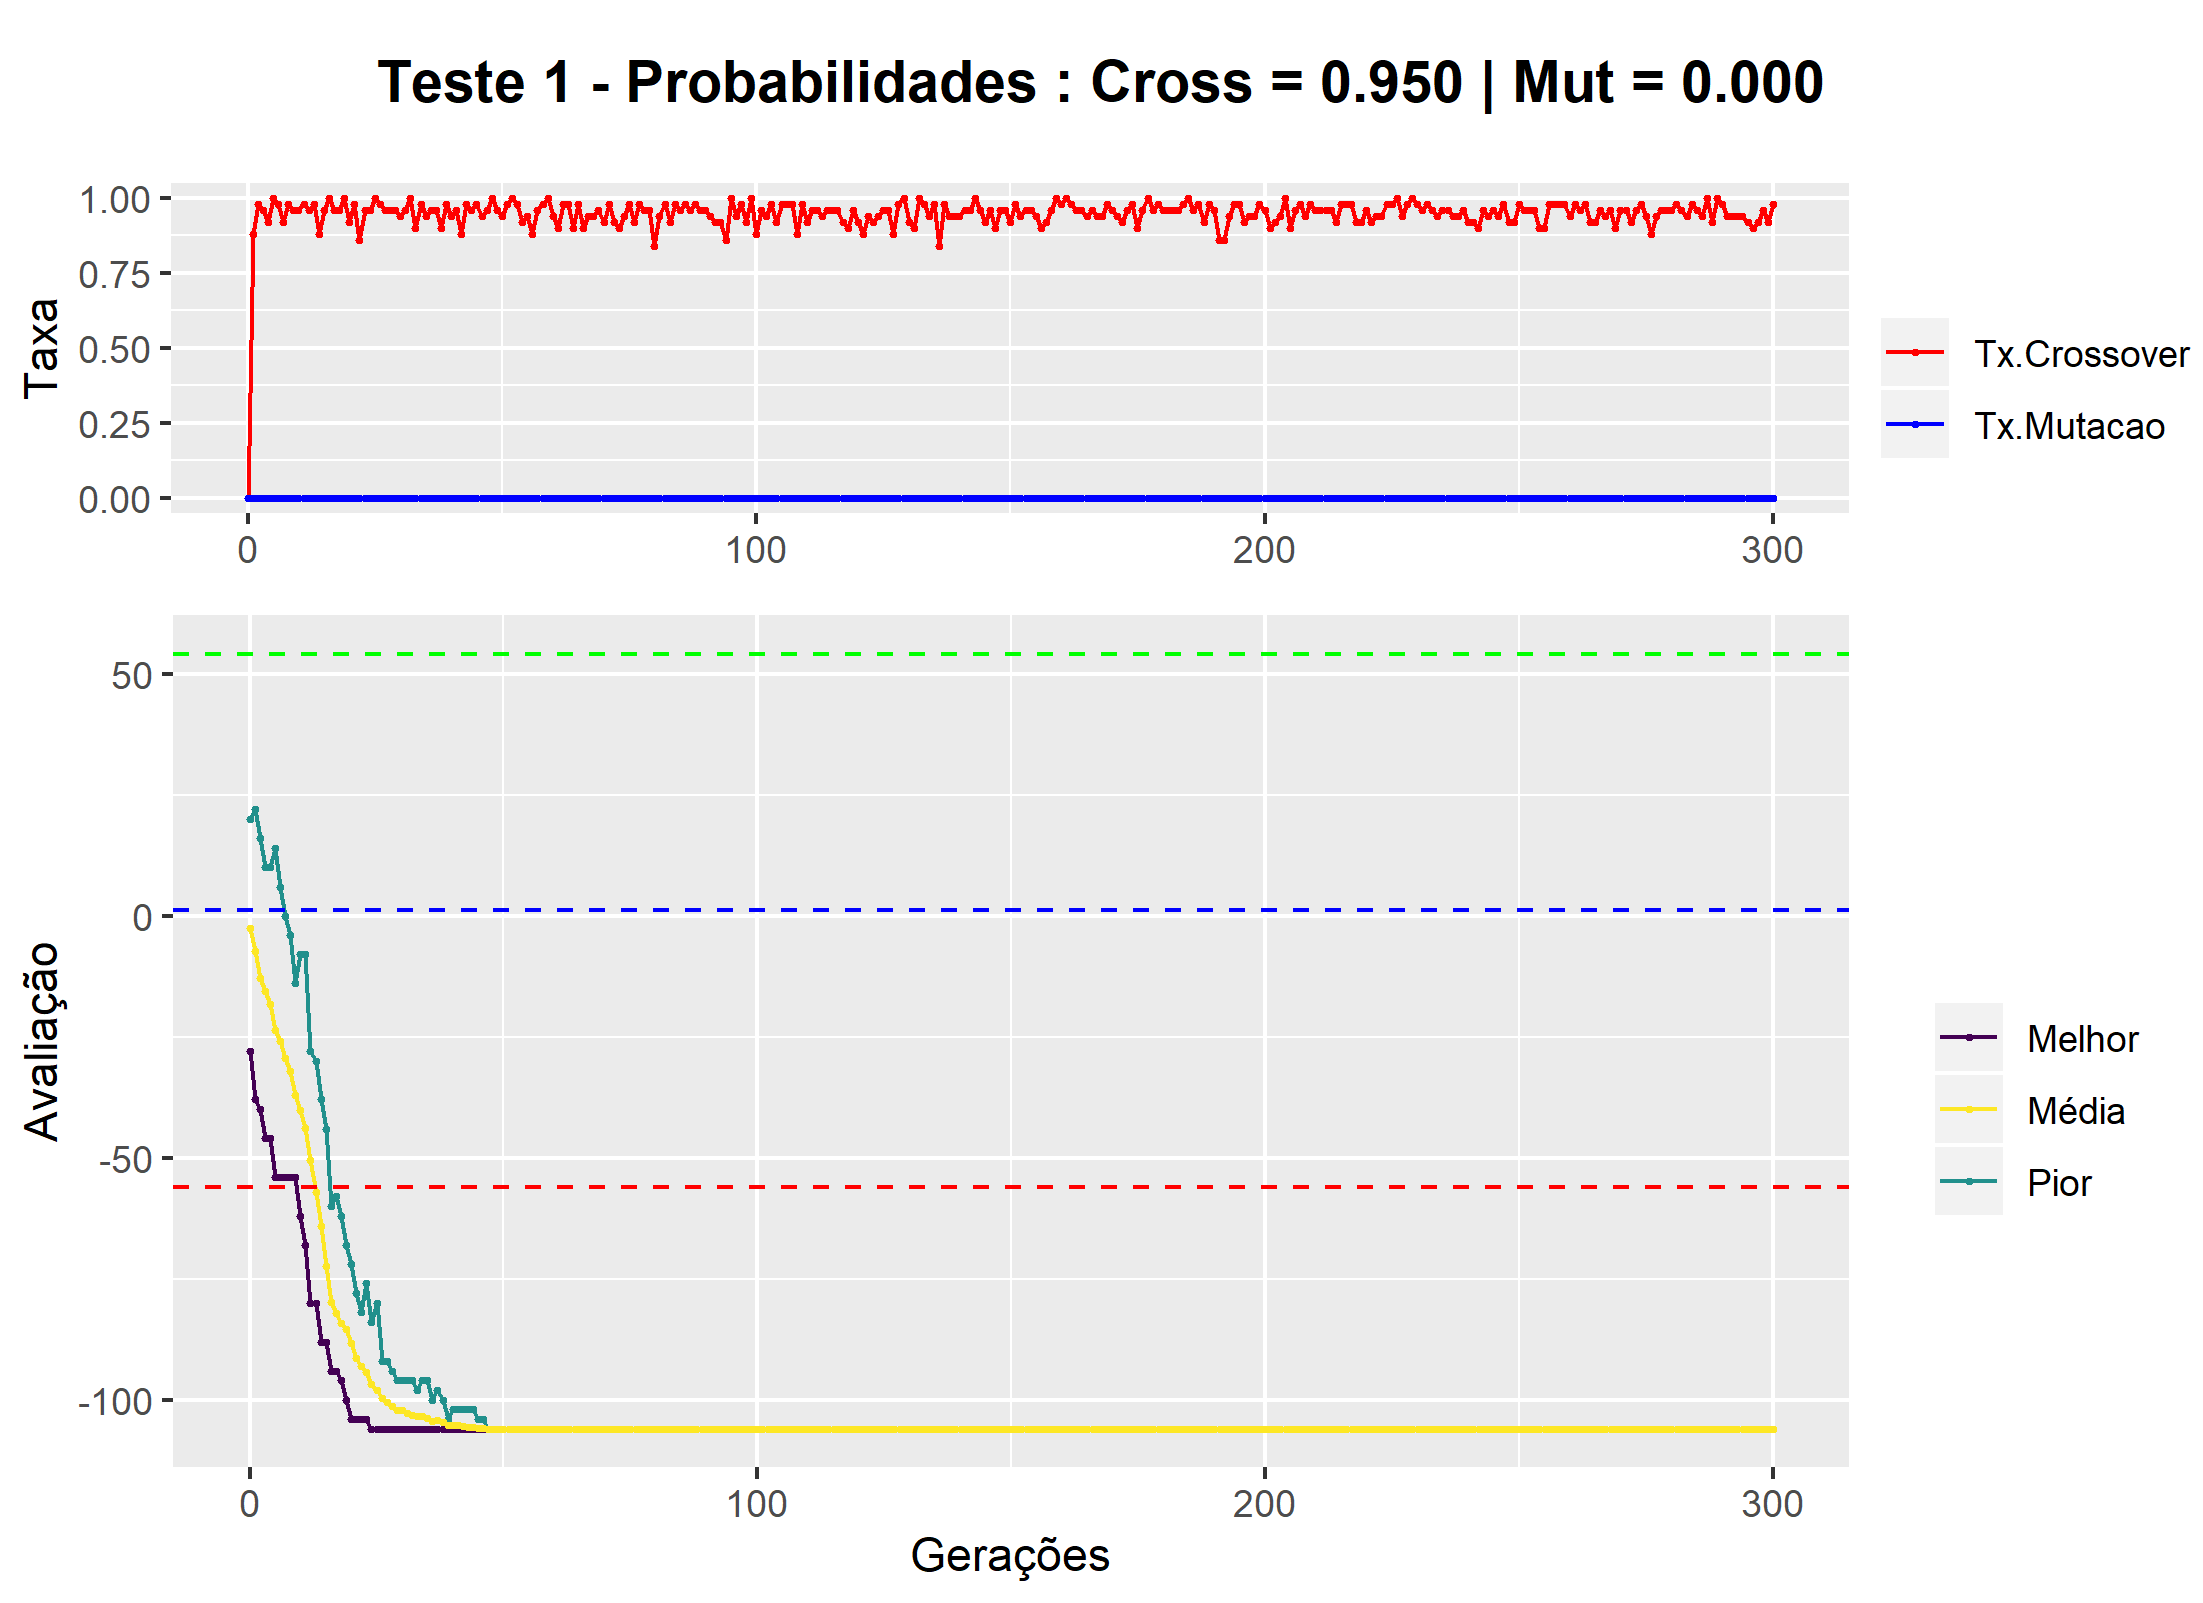
\includegraphics[width=\linewidth]{imagens/graph_pc_0_950_pm_0_000_pop_50_g_300__1.png}
		\caption{}
	\end{subfigure}
	\begin{subfigure}[b]{0.47\linewidth}
		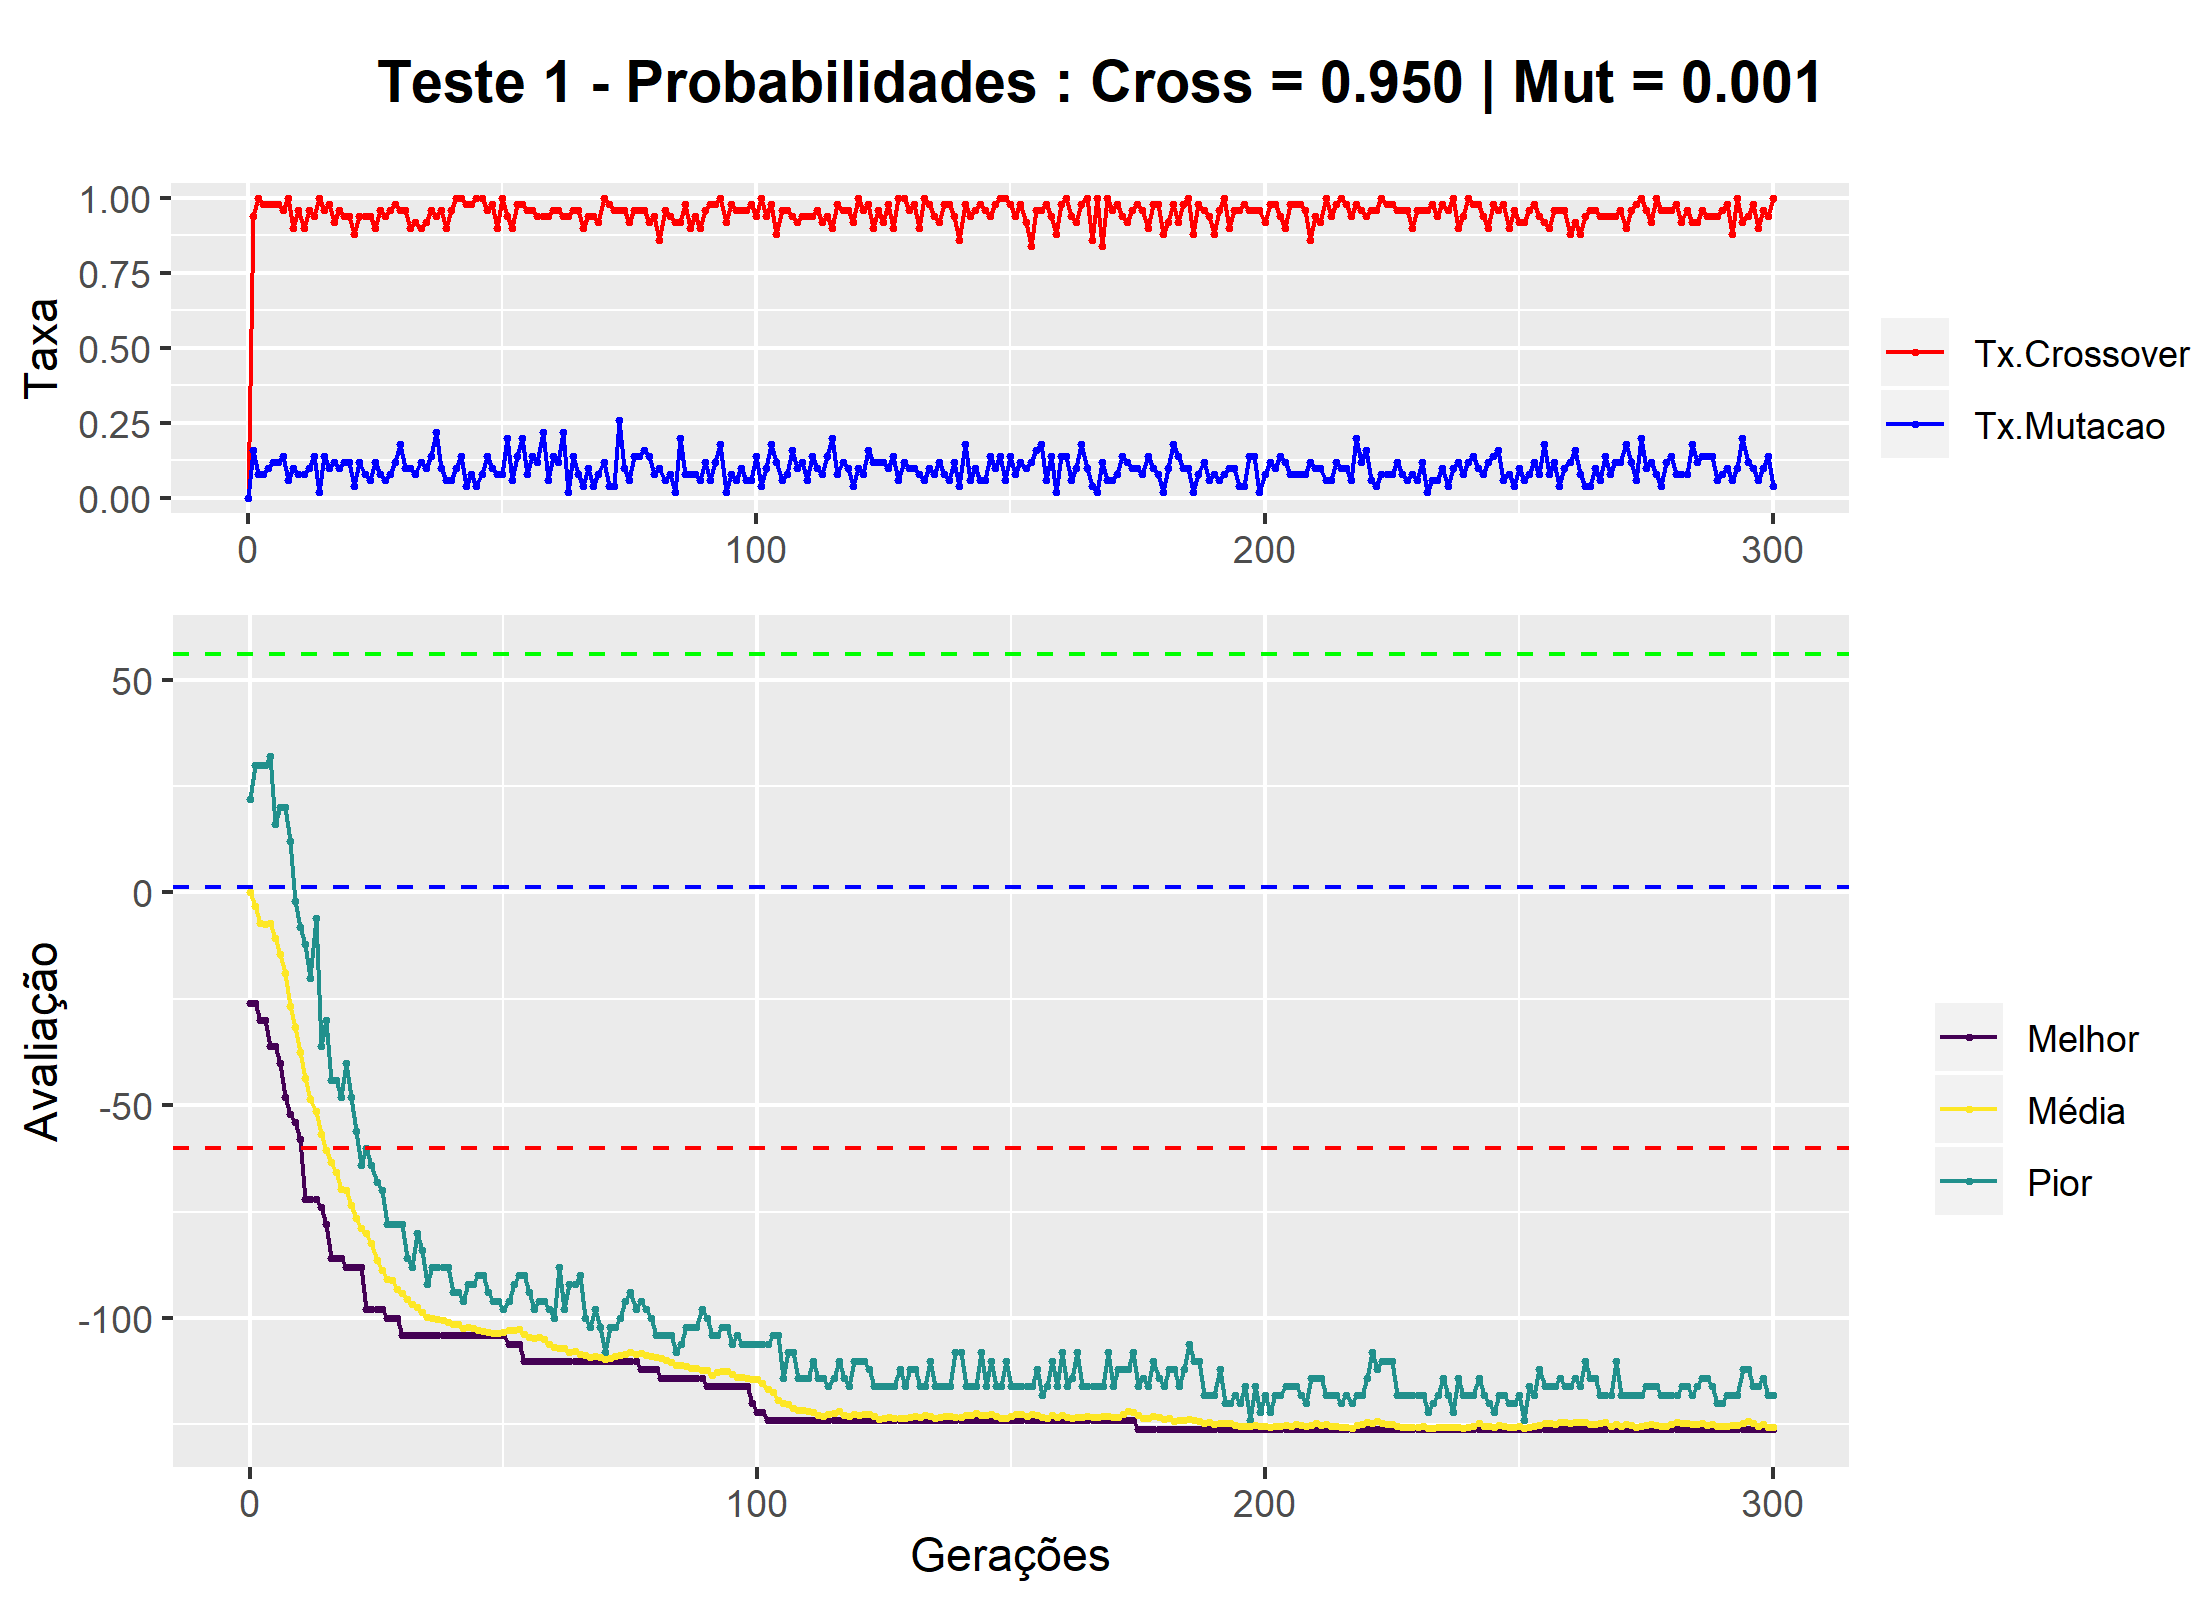
\includegraphics[width=\linewidth]{imagens/graph_pc_0_950_pm_0_001_pop_50_g_300__1.png}
		\caption{}
	\end{subfigure}
	\begin{subfigure}[b]{0.47\linewidth}
		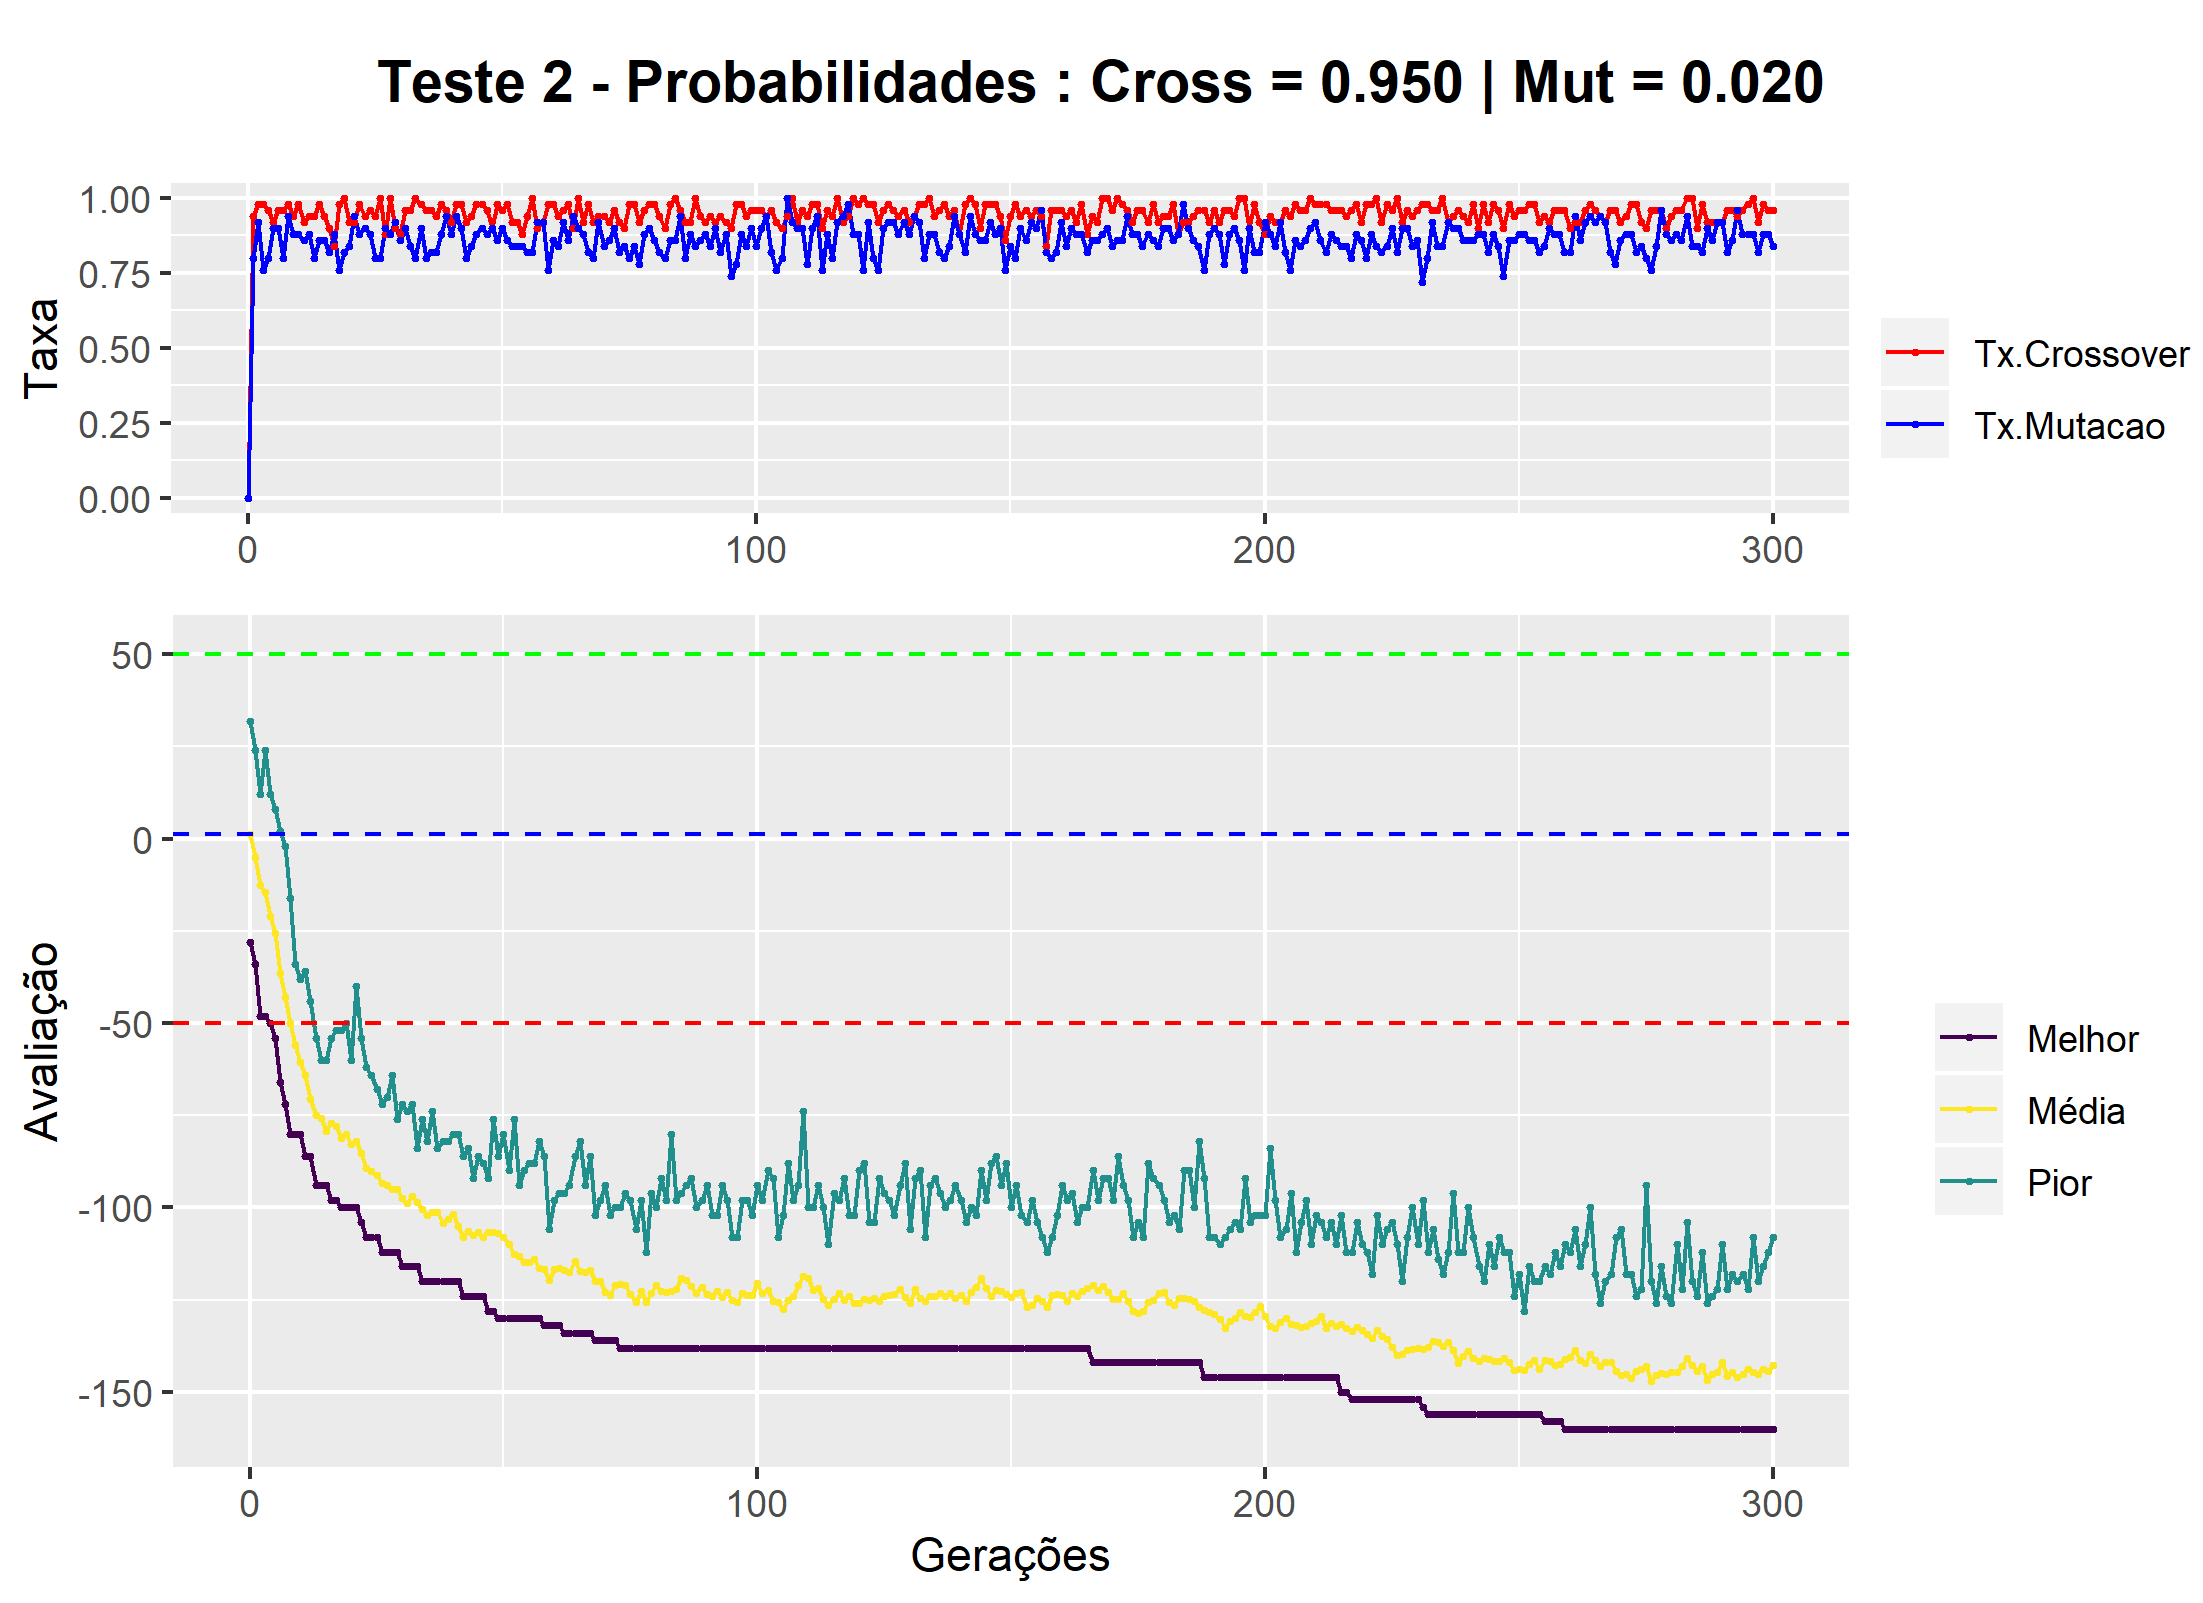
\includegraphics[width=\linewidth]{imagens/graph_pc_0_950_pm_0_020_pop_50_g_300__2.png}
		\caption{}
	\end{subfigure}
	\begin{subfigure}[b]{0.47\linewidth}
		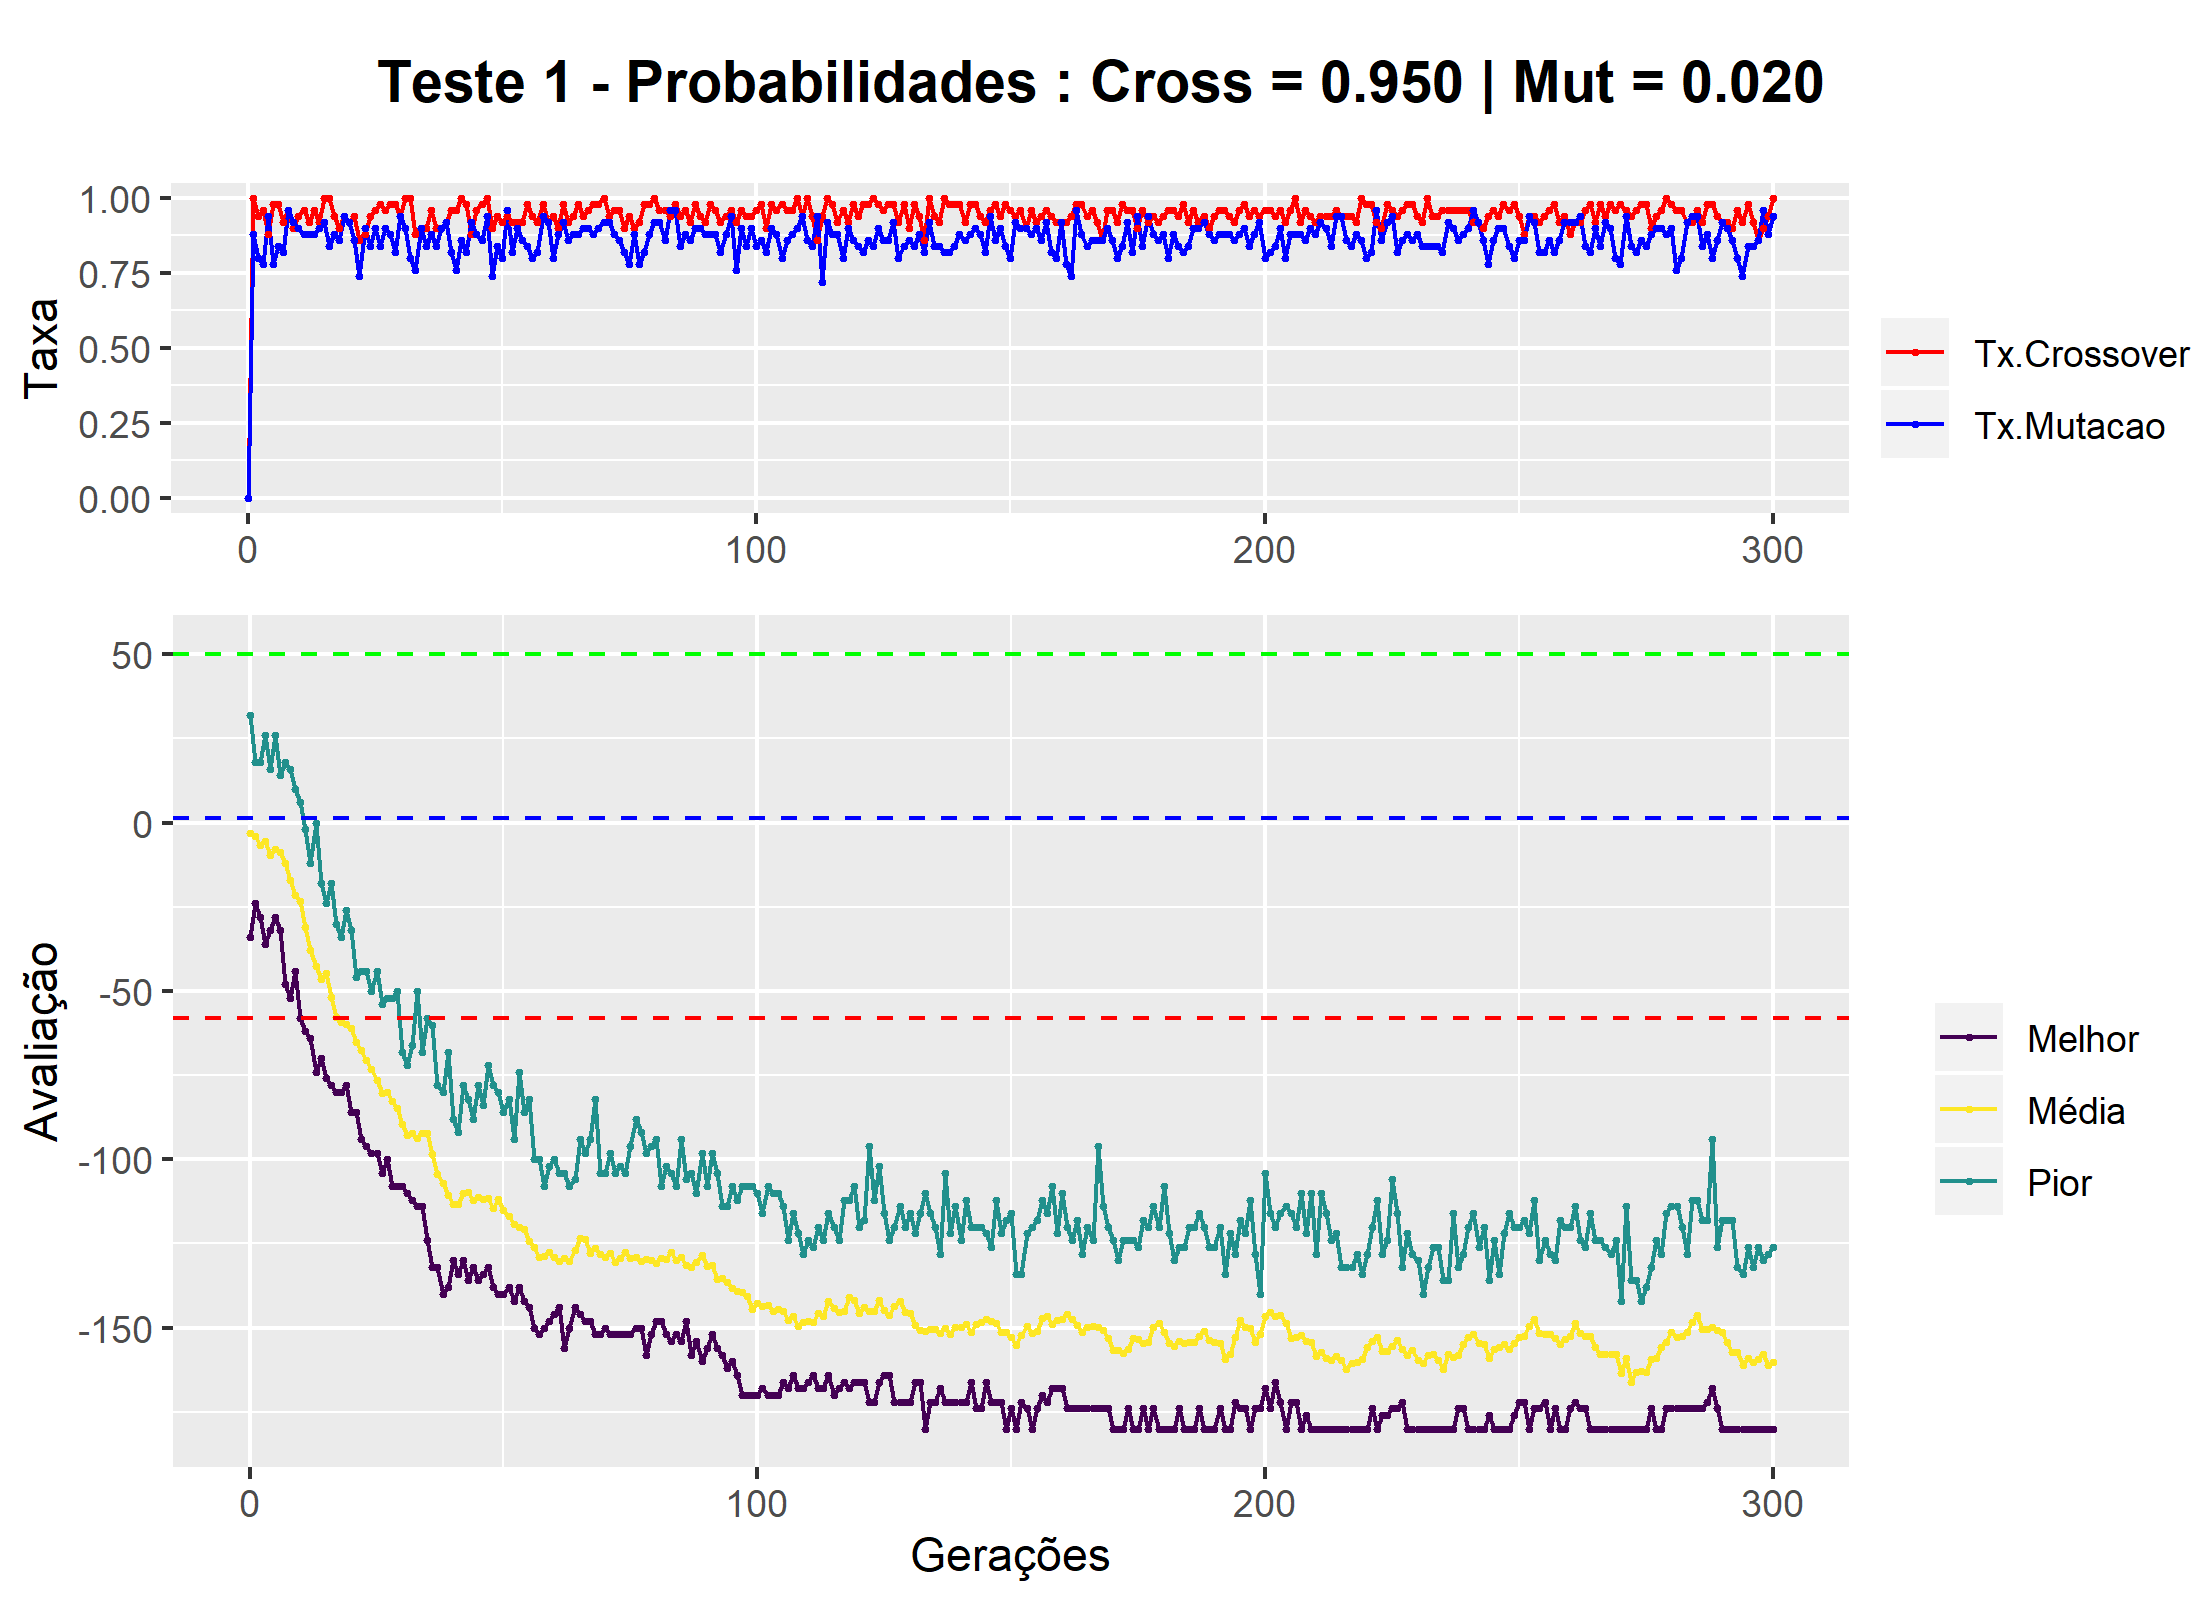
\includegraphics[width=\linewidth]{imagens/graph_pc_0_950_pm_0_020_pop_50_g_300__1_noelite.png}
		\caption{Sem elitismo}
	\end{subfigure}
\caption{Evolução do algoritmo genético durante gerações}
	\label{fig:evolucaoGA}
\end{figure}

Outros gráficos de resultados podem ser vistos na \autoref{fig:evolucaoGA2} do \refanexo{chap:anexos}.


%\chapter{Conteúdos específicos do modelo de trabalho acadêmico}\label{cap_trabalho_academico}
%
%\section{Quadros}
%
%Este modelo vem com o ambiente \texttt{quadro} e impressão de Lista de quadros 
%configurados por padrão. Verifique um exemplo de utilização:
%
%\begin{quadro}[htb]
%\caption{\label{quadro_exemplo}Exemplo de quadro}
%\begin{tabular}{|c|c|c|c|}
%	\hline
%	\textbf{Pessoa} & \textbf{Idade} & \textbf{Peso} & \textbf{Altura} \\ \hline
%	Marcos & 26    & 68   & 178    \\ \hline
%	Ivone  & 22    & 57   & 162    \\ \hline
%	...    & ...   & ...  & ...    \\ \hline
%	Sueli  & 40    & 65   & 153    \\ \hline
%\end{tabular}
%\fonte{Autor.}
%\end{quadro}
%
%Este parágrafo apresenta como referenciar o quadro no texto, requisito
%obrigatório da ABNT. 
%Primeira opção, utilizando \texttt{autoref}: Ver o \autoref{quadro_exemplo}. 
%Segunda opção, utilizando  \texttt{ref}: Ver o Quadro \ref{quadro_exemplo}.

%% ----------------------------------------------------------
%% PARTE
%% ----------------------------------------------------------
%\part{Referenciais teóricos}
%% ----------------------------------------------------------
%
%% ---
%% Capitulo de revisão de literatura
%% ---
%\chapter{Lorem ipsum dolor sit amet}
%% ---
%
%% ---
%\section{Aliquam vestibulum fringilla lorem}
%% ---
%
%\lipsum[1]
%
%\lipsum[2-3]

% ----------------------------------------------------------
% PARTE
% ----------------------------------------------------------
%\part{Resultados}
% ----------------------------------------------------------

%% ---
%% primeiro capitulo de Resultados
%% ---
%\chapter{Lectus lobortis condimentum}
%% ---
%
%% ---
%\section{Vestibulum ante ipsum primis in faucibus orci luctus et ultrices
%posuere cubilia Curae}
%% ---
%
%\lipsum[21-22]
%
%% ---
%% segundo capitulo de Resultados
%% ---
%\chapter{Nam sed tellus sit amet lectus urna ullamcorper tristique interdum
%elementum}
%% ---
%
%% ---
%\section{Pellentesque sit amet pede ac sem eleifend consectetuer}
%% ---
%
%\lipsum[24]

% ----------------------------------------------------------
% Finaliza a parte no bookmark do PDF
% para que se inicie o bookmark na raiz
% e adiciona espaço de parte no Sumário
% ----------------------------------------------------------
\phantompart

% ---
% Conclusão
% ---
\chapter{Conclusão}
% ---
%\lipsum[31-33]
O algoritmo genético é uma outra ferramenta que dispomos pela busca de soluções ótimas. Como visto na literatura, podemos considerar que na verdade é um algoritmo com foco em busca de soluções satisfatórias do que exatamente da solução ótima. Uma das vantagens está na facilidade de implementação do algoritmo, porém possui parâmetros de configuração que ainda não se conhece formas de definir analiticamente os melhores valores, além de dependerem das condições do problema a ser resolvido. Com isso a maior parte dos trabalhos se baseiam em resultados empíricos para ajuste dos parâmetros. Foi visto que o GA também apresenta algumas dificuldades com certas condições, mas que podem ser amenizadas se propriamente codificado e parametrizado. 

Nos testes realizados, o GA se mostrou bem mais eficiente que a busca aleatória, alcançando resultados mais expressivos. Portanto em problemas que por limitações inerentes seriam usados o algoritmo de busca aleatória, o algoritmo genético se apresenta como uma outra abordagem possível. 

Ficou demonstrado que é muito importante as escolhas feitas para a arquitetura do GA e seus parâmetros podem definir o sucesso do algoritmo. No teste sobre o modelo de Ising, percebeu-se que a utilização de uma função de avaliação, que não era a mais apropriada, resultou em ineficiência do algoritmo obtendo resultados iguais e até inferiores que a busca aleatória, fato contornado usando outra função. Esse tipo de detalhe é exatamente o \citeauthor{Linden2008} menciona sobre quanto mais informação sobre o problema conseguir inserir no algoritmo, melhor será a resposta, e por isso não existe uma padrão do GA que seja ideal para todos os problemas.

Outro conceito que impôs diferença nos resultados foi o uso do elitismo, pois ao manter os melhores cromossomos de uma geração para outra, sustentou-se o melhor resultado até o fim do processo. Sem o elitismo era possível ver nos gráficos que o melhor cromossomo em gerações \(t+1\) ficavam com pior resultado que o o melhor da geração \(t\).

No modelo de Ising, o algoritmo mostrou através da análise das médias e variâncias, que caminhava para uma convergência, e com boa probabilidade de se tiver gerações suficientes, encontrar o estado de menor energia

As aplicações para o GA são as mais variadas, podendo ser usado em problemas de busca de máximo ou mínimo de funções multivariadas e também com multiobjetivos, na busca de ordenações mais eficientes, como é o caso do problema do caixeiro viajante, e programação genética, onde o GA consegue criar pequenos algoritmos para solução de problemas. 

Umas das aplicações interessantes para o algoritmo é na busca dos coeficientes de uma rede neural. Para as redes usadas em processos de \textit{machine learning} para classificação, pode ser usado de forma a determinar os coeficientes iniciais para o algoritmo de \textit{backpropagation}, que por ser uma função com vários máximos locais, dependendo do ponto inicial utilizado pode ficar preso a um que não seja o máximo global. Normalmente o ponto inicial é definido aleatoriamente, e nesse sentido que poderia ser usado o GA, que teria uma população definida por cromossomos de valores reais definindo os coeficientes inicias da rede. Para cada cromossomo poderia ser executado o \textit{backpropagation} e verificado através dos resultados qual obteve melhor taxa de sucesso de classificação, e usado esse valor como função de avaliação.

Ainda com redes neurais, existem os casos que a rede define o comportamento de um sistema em resposta a sensores de entrada. O caso clássico de demonstração dessa aplicação é do treinar o computador para jogar determinado jogo eletrônico. A população fica definida como cromossomos de valores reais com os coeficientes da rede e o resultado da rede só pode ser visto após determinada simulação. A população do GA testada contra o resultado de pontuação, que será a função de avaliação do algoritmo, é evoluída então combinando os melhores resultados e aplicando mutação em alguns.

Outra característica interessante, que ainda pode ser explorada, é a possibilidade de combinar o GA com outro algoritmo de otimização, por exemplo direcionando a mutação para uma busca de máximo local da função de avaliação. Esse pode ser um diferencial combinando a qualidade do GA de encontrar soluções satisfatórias ou próximas a máximos locais e combinar com um algoritmo mais eficiente de maximização local, como o \textit{hill climbing}.

O algoritmo genético ainda precisa ser muito analisado de forma a entender melhor seu mecanismo de funcionamento e dessa forma conseguir determinar os melhores parâmetros, e tem demonstrado certa popularidade com as novas técnicas de AI e \textit{machine learning}.

Para trabalhos futuros podem ser seguido os testes com o modelo proposto de Ising, trabalhando com contornos e busca de soluções para acoplamentos do modelo, também podem ser explorados as técnicas de combinar com outros métodos. Ainda é necessário também avaliar o algoritmo com relação a seu desempenho computacional e outro passo importante seria o de executar o algoritmo usando paralelismo, pois a fase de avaliação e seleção poderia facilmente ser colocada em tarefas concorrentes, otimizando o tempo de resposta do algoritmo.  


% ----------------------------------------------------------
% ELEMENTOS PÓS-TEXTUAIS
% ----------------------------------------------------------
\postextual
% ----------------------------------------------------------

% ----------------------------------------------------------
% Referências bibliográficas
% ----------------------------------------------------------
%\bibliography{abntex2-modelo-references}
\nocite{LeeJacobson2015} % colocar nessa forma todos aqueles que não foram citados diretamente
\bibliography{TC}

% ----------------------------------------------------------
% Glossário
% ----------------------------------------------------------
%
% Consulte o manual da classe abntex2 para orientações sobre o glossário.
%
%\glossary

% ----------------------------------------------------------
% Apêndices
% ----------------------------------------------------------

% ---
% Inicia os apêndices
% ---
%\begin{apendicesenv}

% Imprime uma página indicando o início dos apêndices
%\partapendices

%% ----------------------------------------------------------
%\chapter{Quisque libero justo}
%% ----------------------------------------------------------
%
%\lipsum[50]
%
%% ----------------------------------------------------------
%\chapter{Nullam elementum urna vel imperdiet sodales elit ipsum pharetra ligula
%ac pretium ante justo a nulla curabitur tristique arcu eu metus}
%% ----------------------------------------------------------
%\lipsum[55-57]

%\end{apendicesenv}
% ---


% ----------------------------------------------------------
% Anexos
% ----------------------------------------------------------

% ---
% Inicia os anexos
% ---
\begin{anexosenv}

% Imprime uma página indicando o início dos anexos
%\partanexos

% ---
% Este capítulo, apresenta os anexos
% ---

\chapter{Resultados}
\label{chap:anexos}

\begin{table}[h!]
	\begin{tabular}{|c|c|c|c|c|}
		\hline
		\textbf{Cromossomo} 	& \textbf{Avaliação} 	& \textbf{\(\mathcal{H}(\sigma) \)}	& \textbf{Taxa de seleção}	& \textbf{Proporção estimada} \\
		\hline
		287	&  222	&  42 	&  0,067	&  0,040 \\ \hline 
		277	&  206	&  26 	&  0,050	&  0,037 \\ \hline 
		280	&  204	&  24 	&  0,033	&  0,037 \\ \hline 
		282	&  204	&  24 	&  0,017	&  0,037 \\ \hline 
		285	&  200	&  20 	&  0,000	&  0,036 \\ \hline 
		276	&  194	&  14 	&  0,000	&  0,035 \\ \hline 
		291	&  194	&  14 	&  0,083	&  0,035 \\ \hline 
		286	&  192	&  12 	&  0,017	&  0,034 \\ \hline 
		293	&  192	&  12 	&  0,033	&  0,034 \\ \hline 
		283	&  190	&  10 	&  0,033	&  0,034 \\ \hline 
		288	&  190	&  10 	&  0,017	&  0,034 \\ \hline 
		289	&  190	&  10 	&  0,000	&  0,034 \\ \hline 
		299	&  188	&  8 	&  0,017	&  0,034 \\ \hline 
		273	&  186	&  6 	&  0,067	&  0,033 \\ \hline 
		300	&  186	&  6 	&  0,017	&  0,033 \\ \hline 
		292	&  184	&  4 	&  0,033	&  0,033 \\ \hline 
		274	&  182	&  2 	&  0,000	&  0,033 \\ \hline 
		297	&  182	&  2 	&  0,067	&  0,033 \\ \hline 
		271	&  180	&  0 	&  0,033	&  0,032 \\ \hline 
		281	&  180	&  0 	&  0,033	&  0,032 \\ \hline 
		295	&  180	&  0 	&  0,050	&  0,032 \\ \hline 
		290	&  178	&  -2 	&  0,050	&  0,032 \\ \hline 
		294	&  178	&  -2 	&  0,033	&  0,032 \\ \hline 
		278	&  176	&  -4 	&  0,017	&  0,032 \\ \hline 
		284	&  176	&  -4 	&  0,067	&  0,032 \\ \hline 
		279	&  174	&  -6 	&  0,033	&  0,031 \\ \hline 
		275	&  172	&  -8 	&  0,067	&  0,031 \\ \hline 
		298	&  172	&  -8 	&  0,033	&  0,031 \\ \hline 
		272	&  164	&  -16 	&  0,000	&  0,029 \\ \hline 
		296	&  160	&  -20 	&  0,033	&  0,029 \\
		\hline
	\end{tabular}
	\caption{Resumo da geração 9 com média de avaliação 185,86 mostrando a taxa de amostragem da seleção e o que era esperado para a proporção usando a função de avaliação da \autoref{eq:Energia_modelo_ising}}
	\label{tab:resumo_GA_H}
\end{table}
\clearpage

\begin{table}[h!]
	\begin{tabular}{|c|c|c|c|c|}
		\hline
		\textbf{Cromossomo} 	& \textbf{Avaliação} 	& \textbf{\(\mathcal{H}(\sigma) \)}	& \textbf{Taxa de seleção}	& \textbf{Proporção estimada} \\
		\hline
		178	&  6,69		&  -38 &  0,100	&  0,063\\ \hline
		160	&  6,05		&  -36 &  0,100	&  0,057\\ \hline
		159	&  5,47		&  -34 &  0,033	&  0,052\\ \hline
		166	&  5,47		&  -34 &  0,067	&  0,052\\ \hline
		162	&  4,95		&  -32 &  0,067	&  0,047\\ \hline
		171	&  4,95		&  -32 &  0,000	&  0,047\\ \hline
		180	&  4,95		&  -32 &  0,033	&  0,047\\ \hline
		167	&  4,48		&  -30 &  0,050	&  0,042\\ \hline
		175	&  4,48		&  -30 &  0,017	&  0,042\\ \hline
		161	&  4,06		&  -28 &  0,050	&  0,038\\ \hline
		163	&  4,06		&  -28 &  0,033	&  0,038\\ \hline
		169	&  4,06		&  -28 &  0,017	&  0,038\\ \hline
		151	&  3,67		&  -26 &  0,050	&  0,035\\ \hline
		155	&  3,67		&  -26 &  0,033	&  0,035\\ \hline
		170	&  3,32		&  -24 &  0,017	&  0,031\\ \hline
		176	&  3,32		&  -24 &  0,050	&  0,031\\ \hline
		153	&  3,00		&  -22 &  0,067	&  0,028\\ \hline
		157	&  3,00		&  -22 &  0,033	&  0,028\\ \hline
		174	&  3,00		&  -22 &  0,050	&  0,028\\ \hline
		152	&  2,72		&  -20 &  0,000	&  0,026\\ \hline
		164	&  2,72		&  -20 &  0,050	&  0,026\\ \hline
		165	&  2,72		&  -20 &  0,000	&  0,026\\ \hline
		158	&  2,46		&  -18 &  0,017	&  0,023\\ \hline
		154	&  2,23		&  -16 &  0,033	&  0,021\\ \hline
		168	&  2,01		&  -14 &  0,000	&  0,019\\ \hline
		173	&  2,01		&  -14 &  0,000	&  0,019\\ \hline
		156	&  1,82		&  -12 &  0,033	&  0,017\\ \hline
		179	&  1,82		&  -12 &  0,000	&  0,017\\ \hline
		172	&  1,22		&  -4 &  0,000	&  0,012\\ \hline
		177	&  1,11		&  -2 &  0,000	&  0,010\\
		\hline
	\end{tabular}
	\caption{Resumo da geração 5 com média de avaliação 3.516 mostrando a taxa de amostragem da seleção e o que era esperado para a proporção usando a função de avaliação da \autoref{eq:selecao_modelo_ising}}
	\label{tab:resumo_GA_expH}
\end{table}

\clearpage
\begin{figure}[h!]
	\centering
	\begin{subfigure}[b]{0.47\linewidth}
		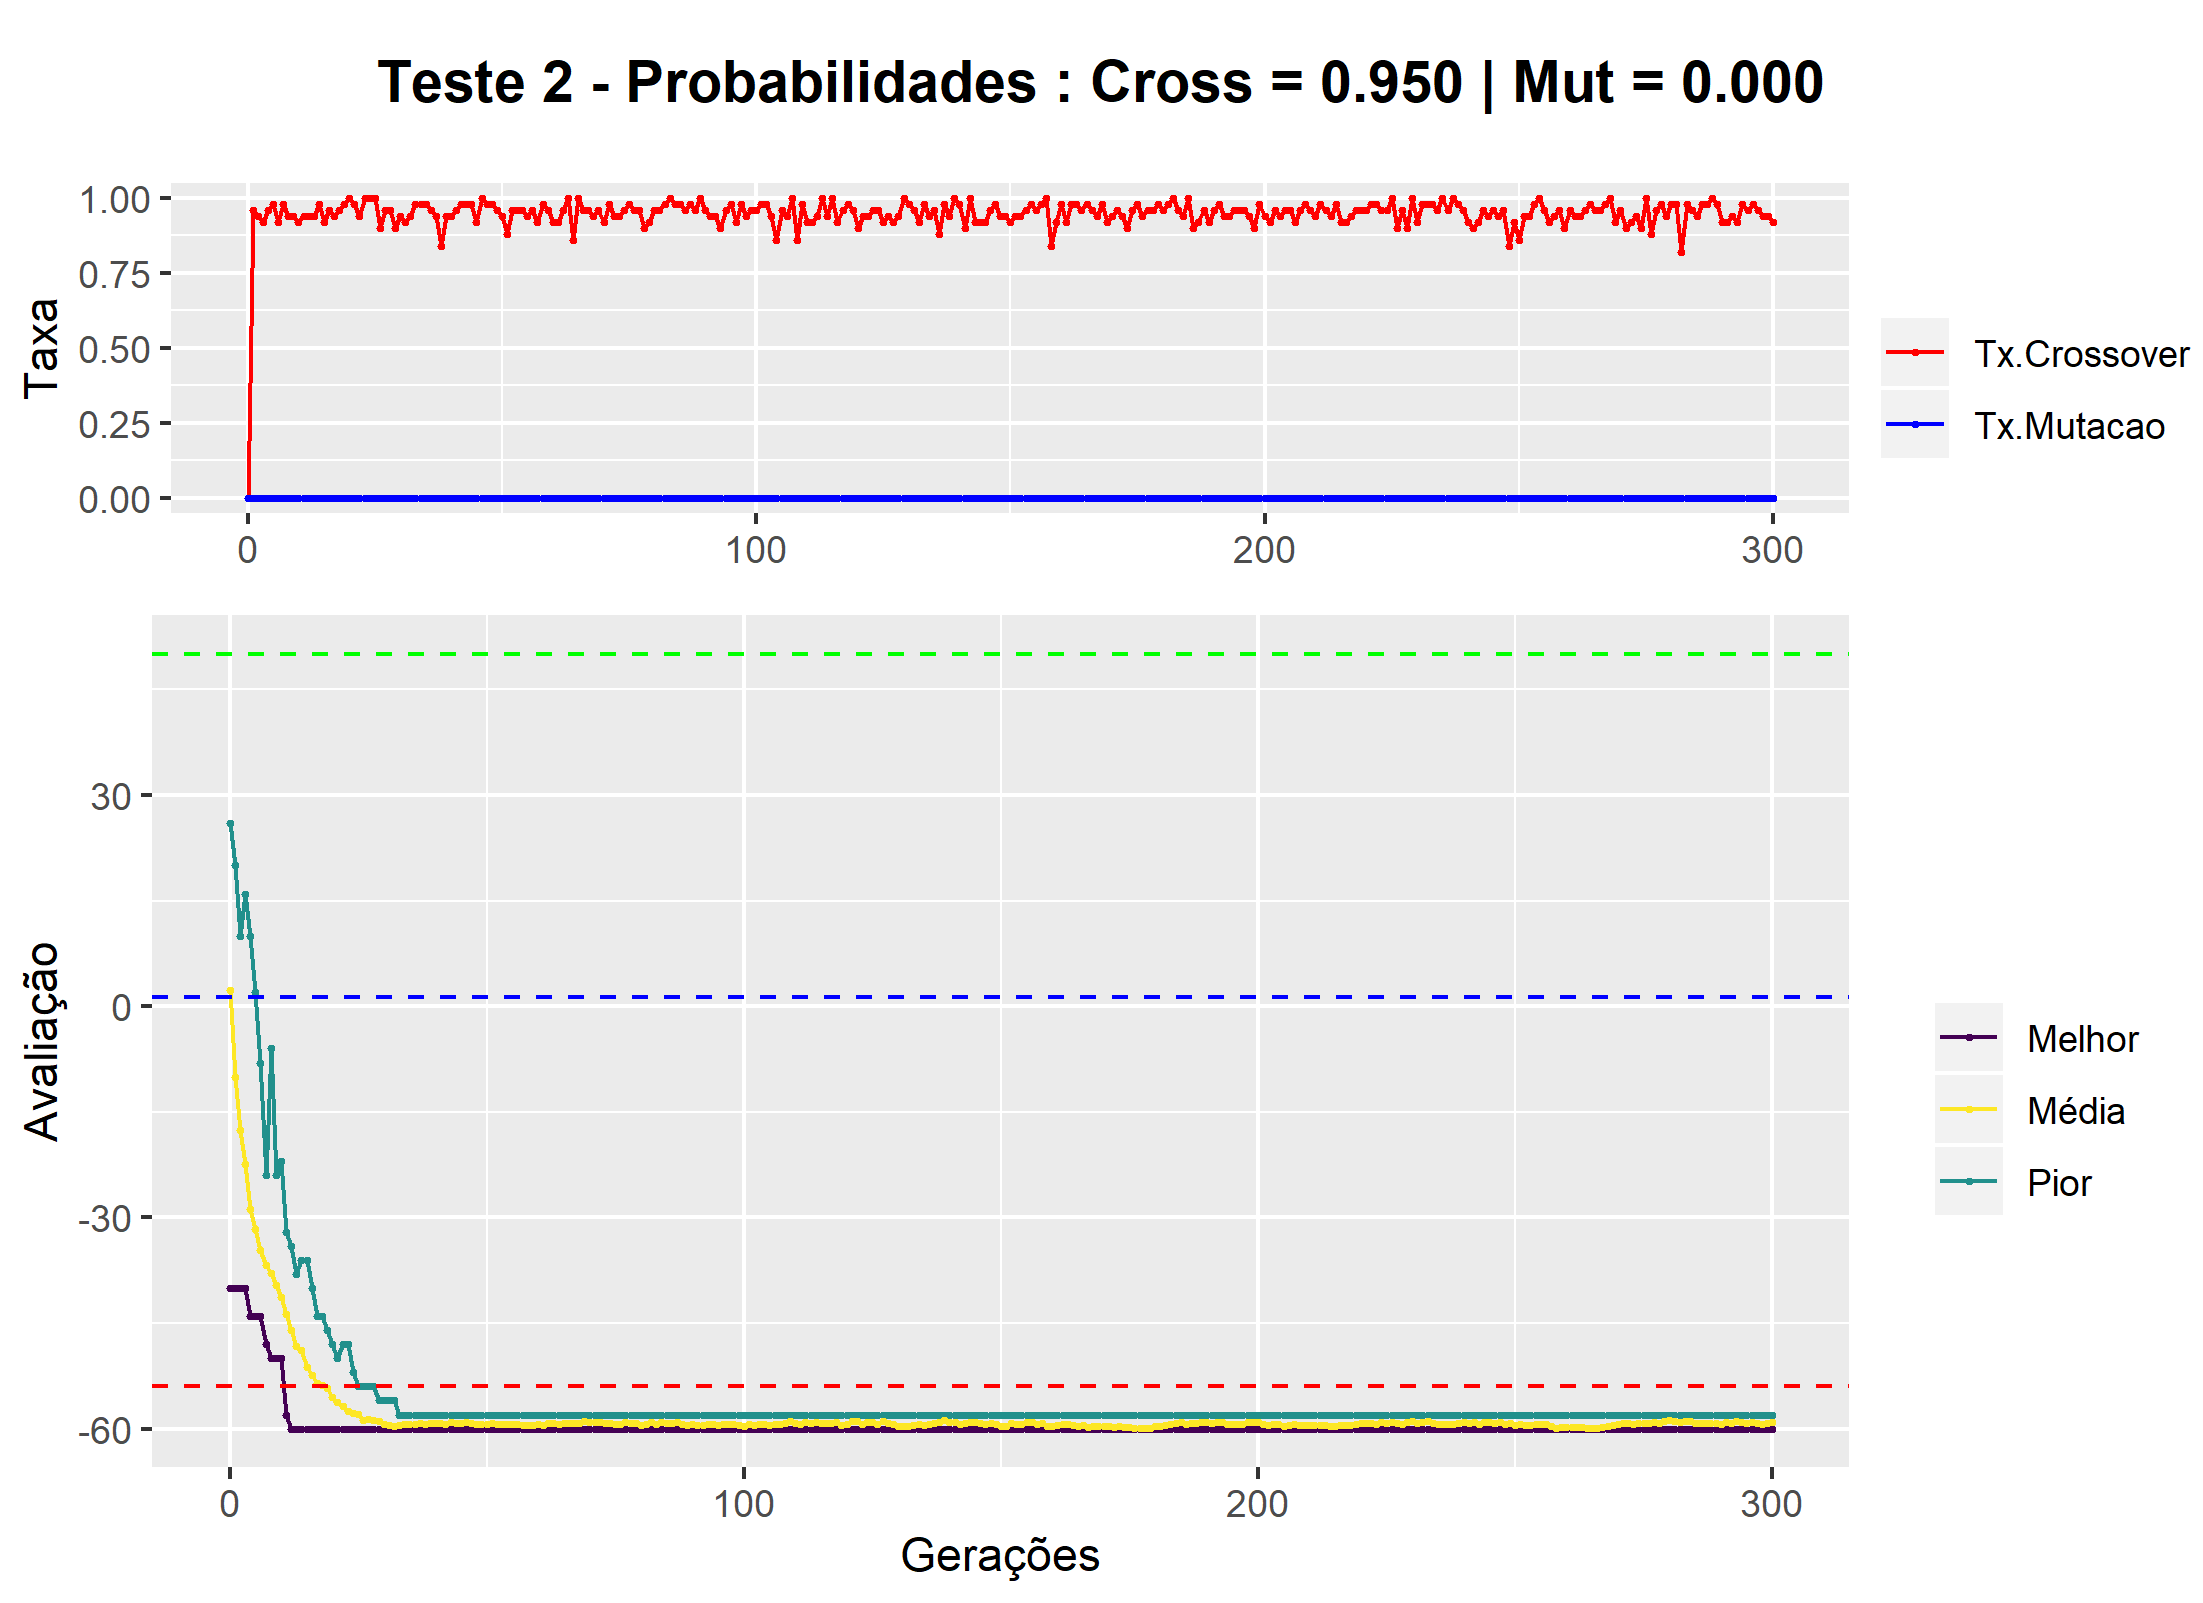
\includegraphics[width=\linewidth]{imagens/graph_pc_0_950_pm_0_000_pop_50_g_300__2.png}
		\caption{}
	\end{subfigure}
	\begin{subfigure}[b]{0.47\linewidth}
		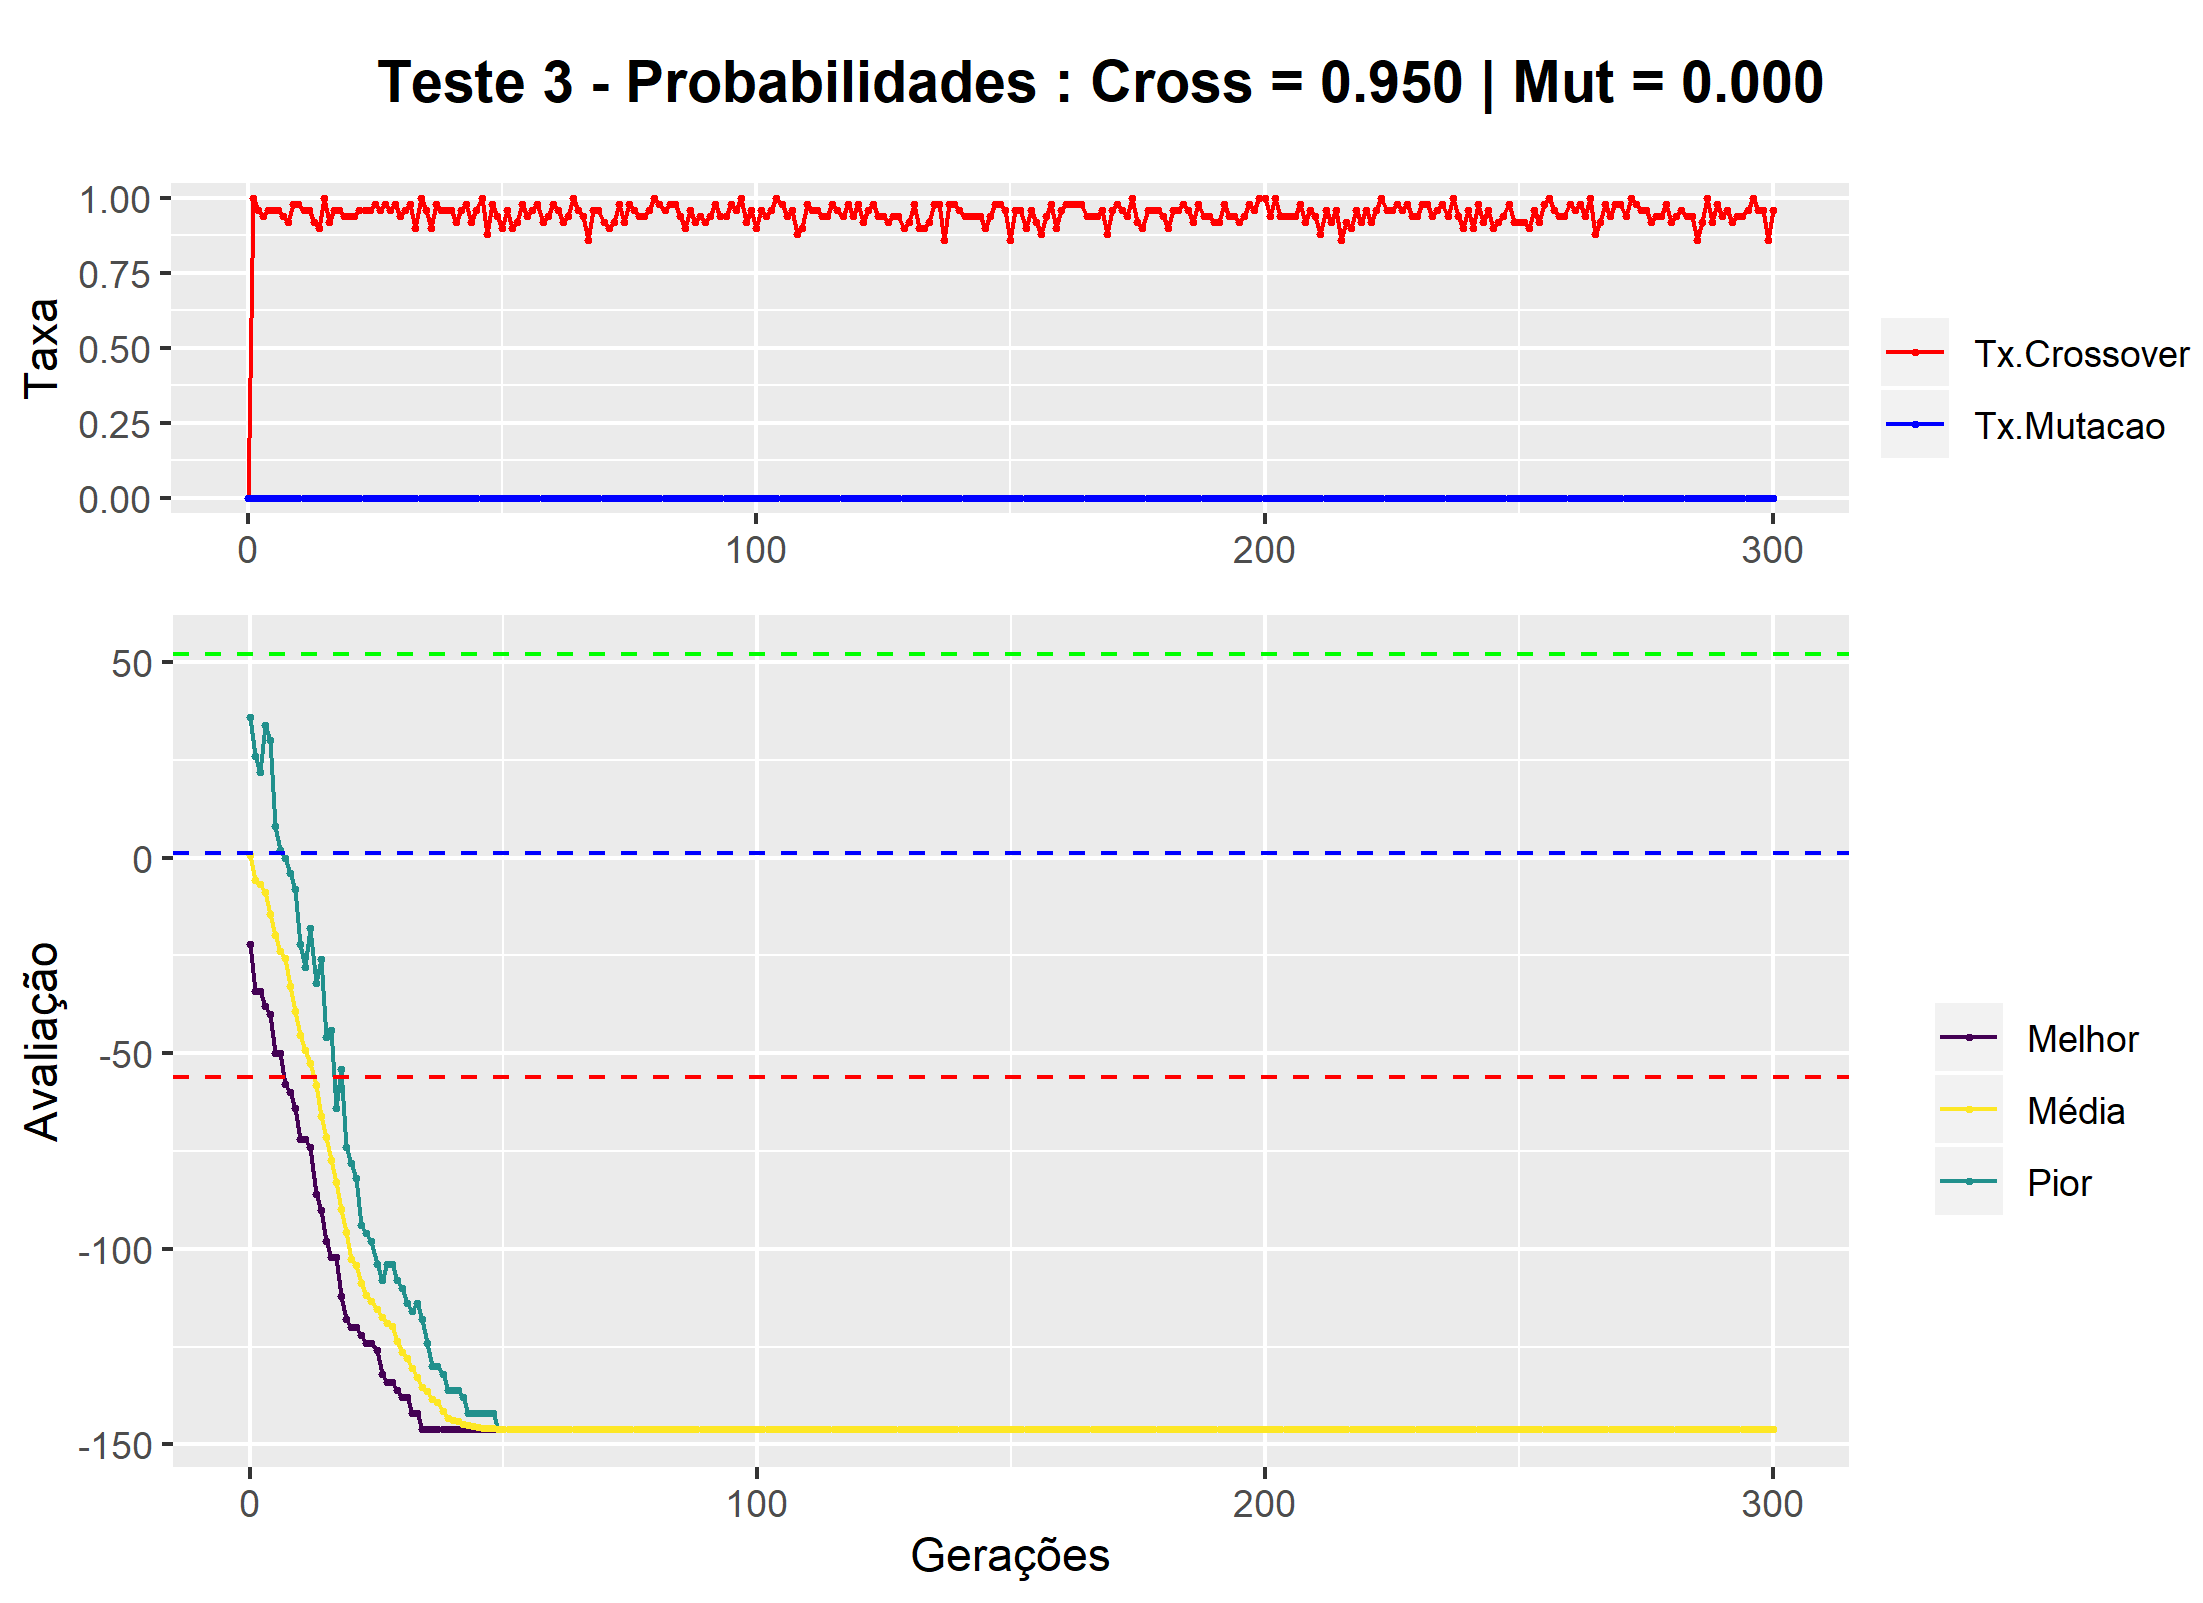
\includegraphics[width=\linewidth]{imagens/graph_pc_0_950_pm_0_000_pop_50_g_300__3.png}
		\caption{}
	\end{subfigure}
	\begin{subfigure}[b]{0.47\linewidth}
		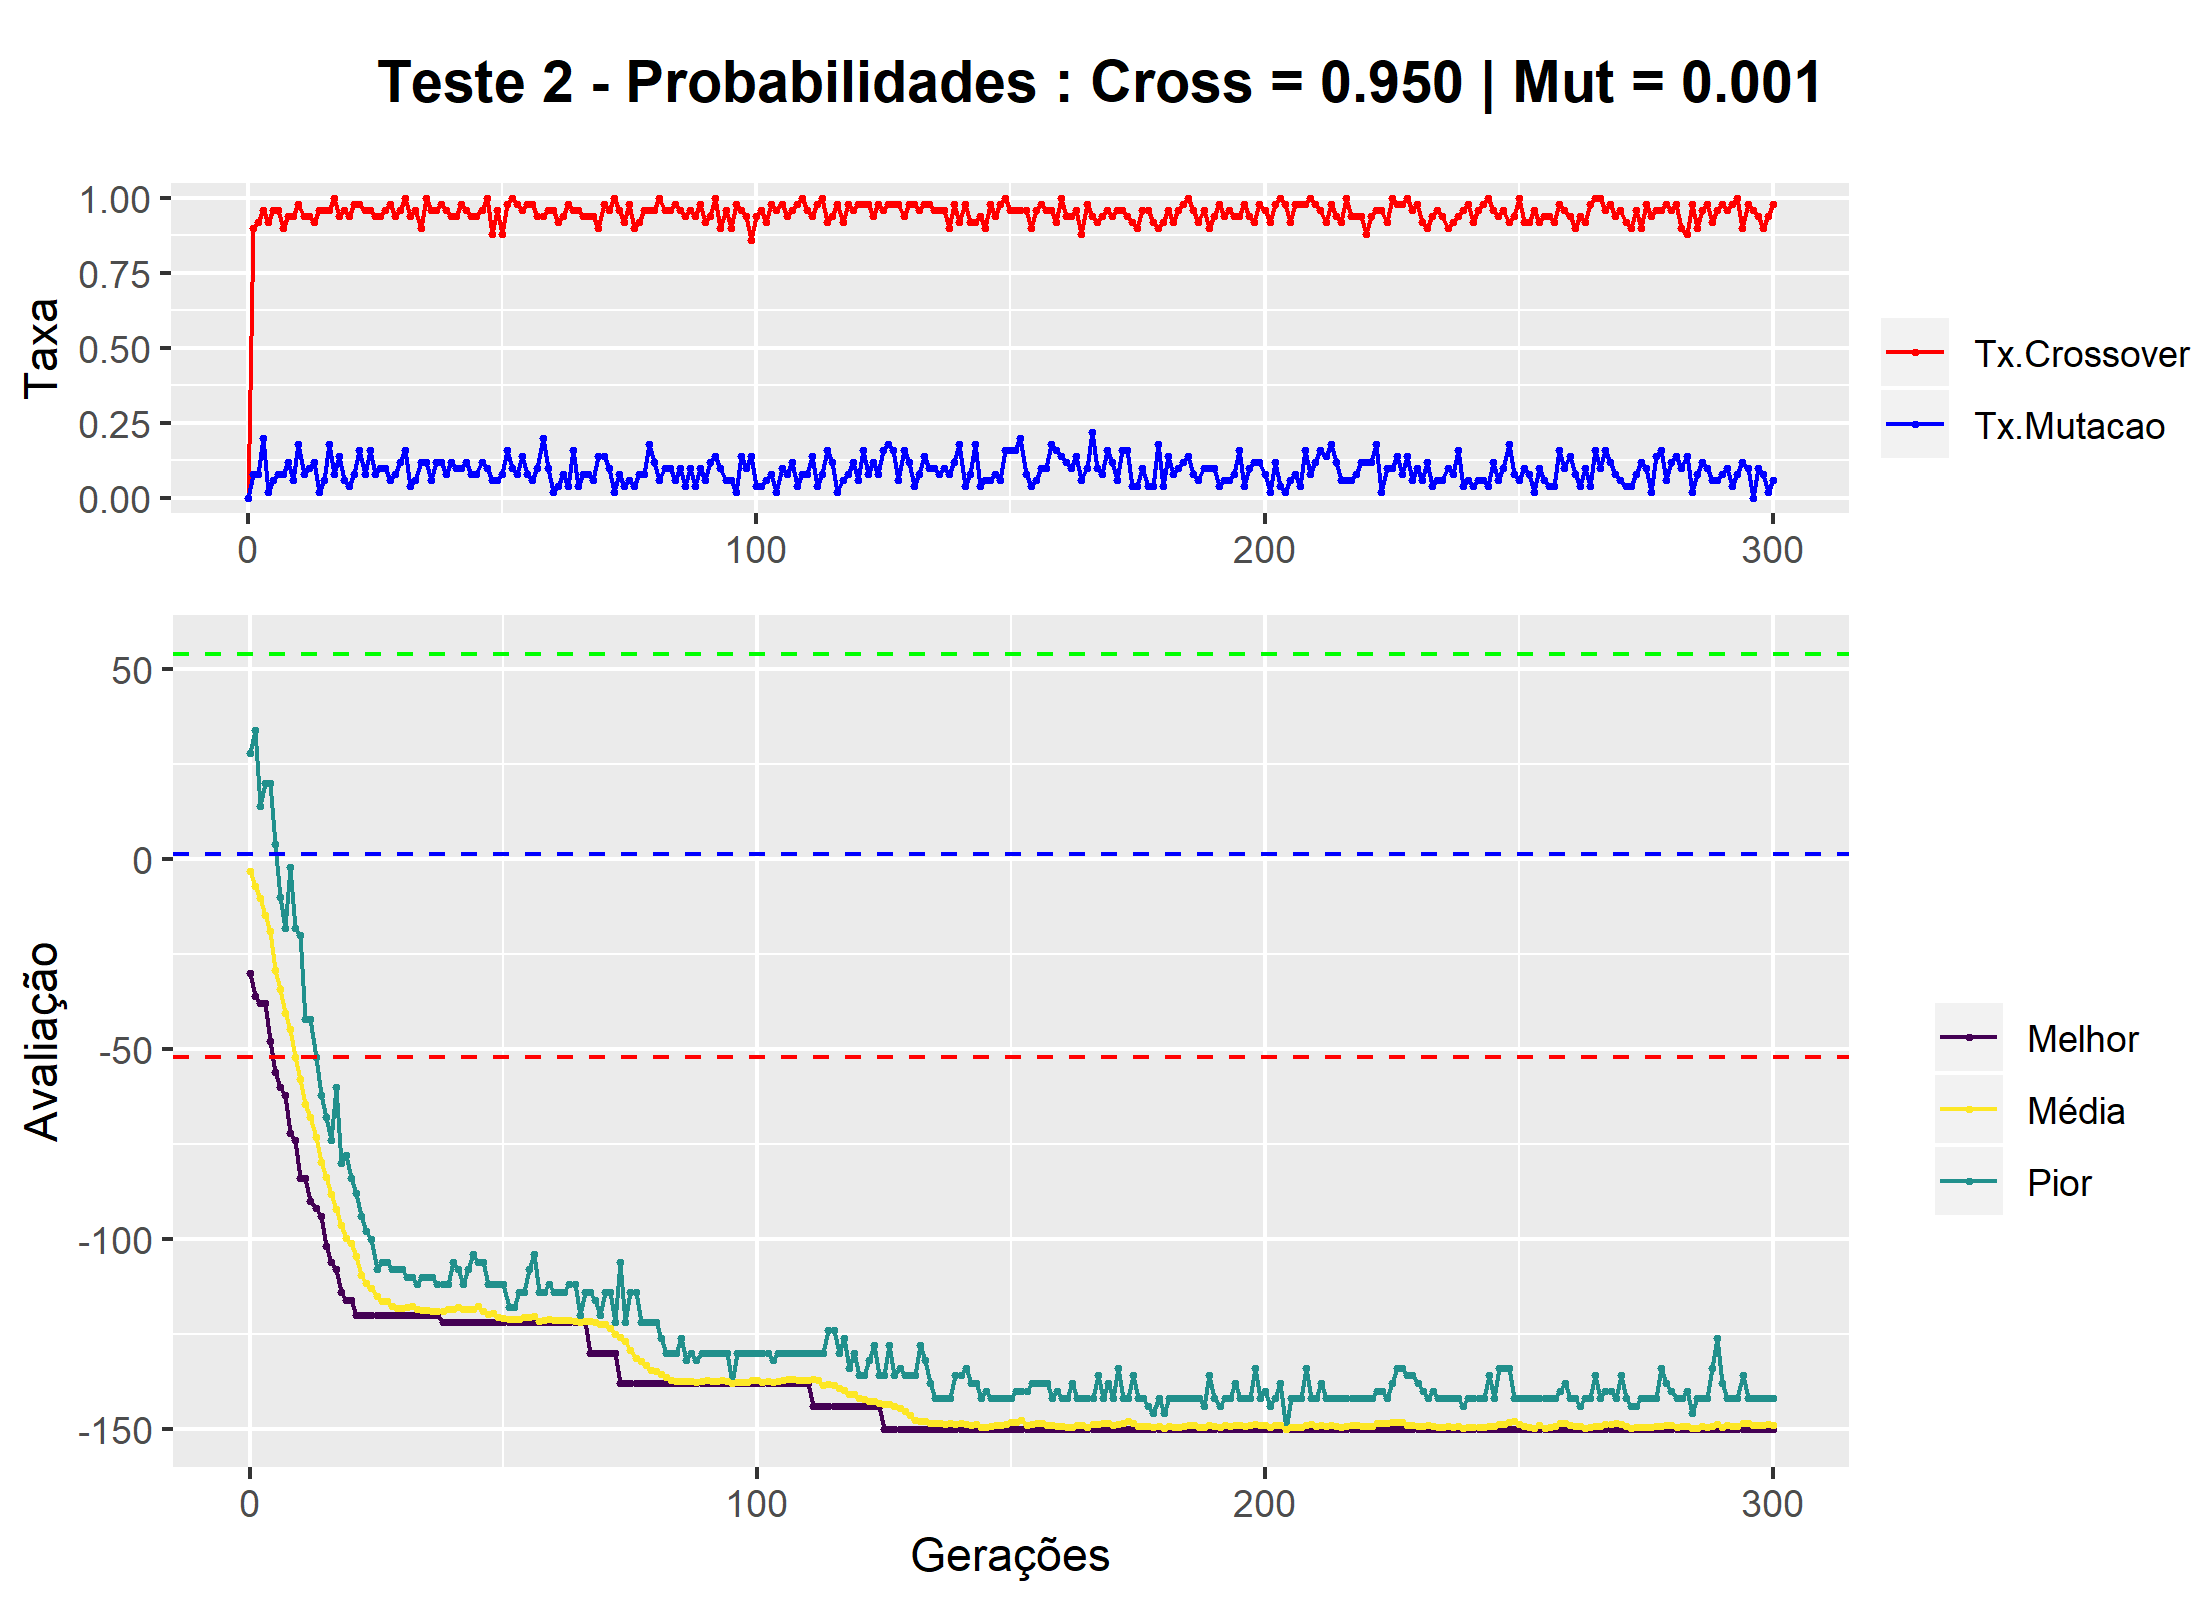
\includegraphics[width=\linewidth]{imagens/graph_pc_0_950_pm_0_001_pop_50_g_300__2.png}
		\caption{}
	\end{subfigure}
	\begin{subfigure}[b]{0.47\linewidth}
		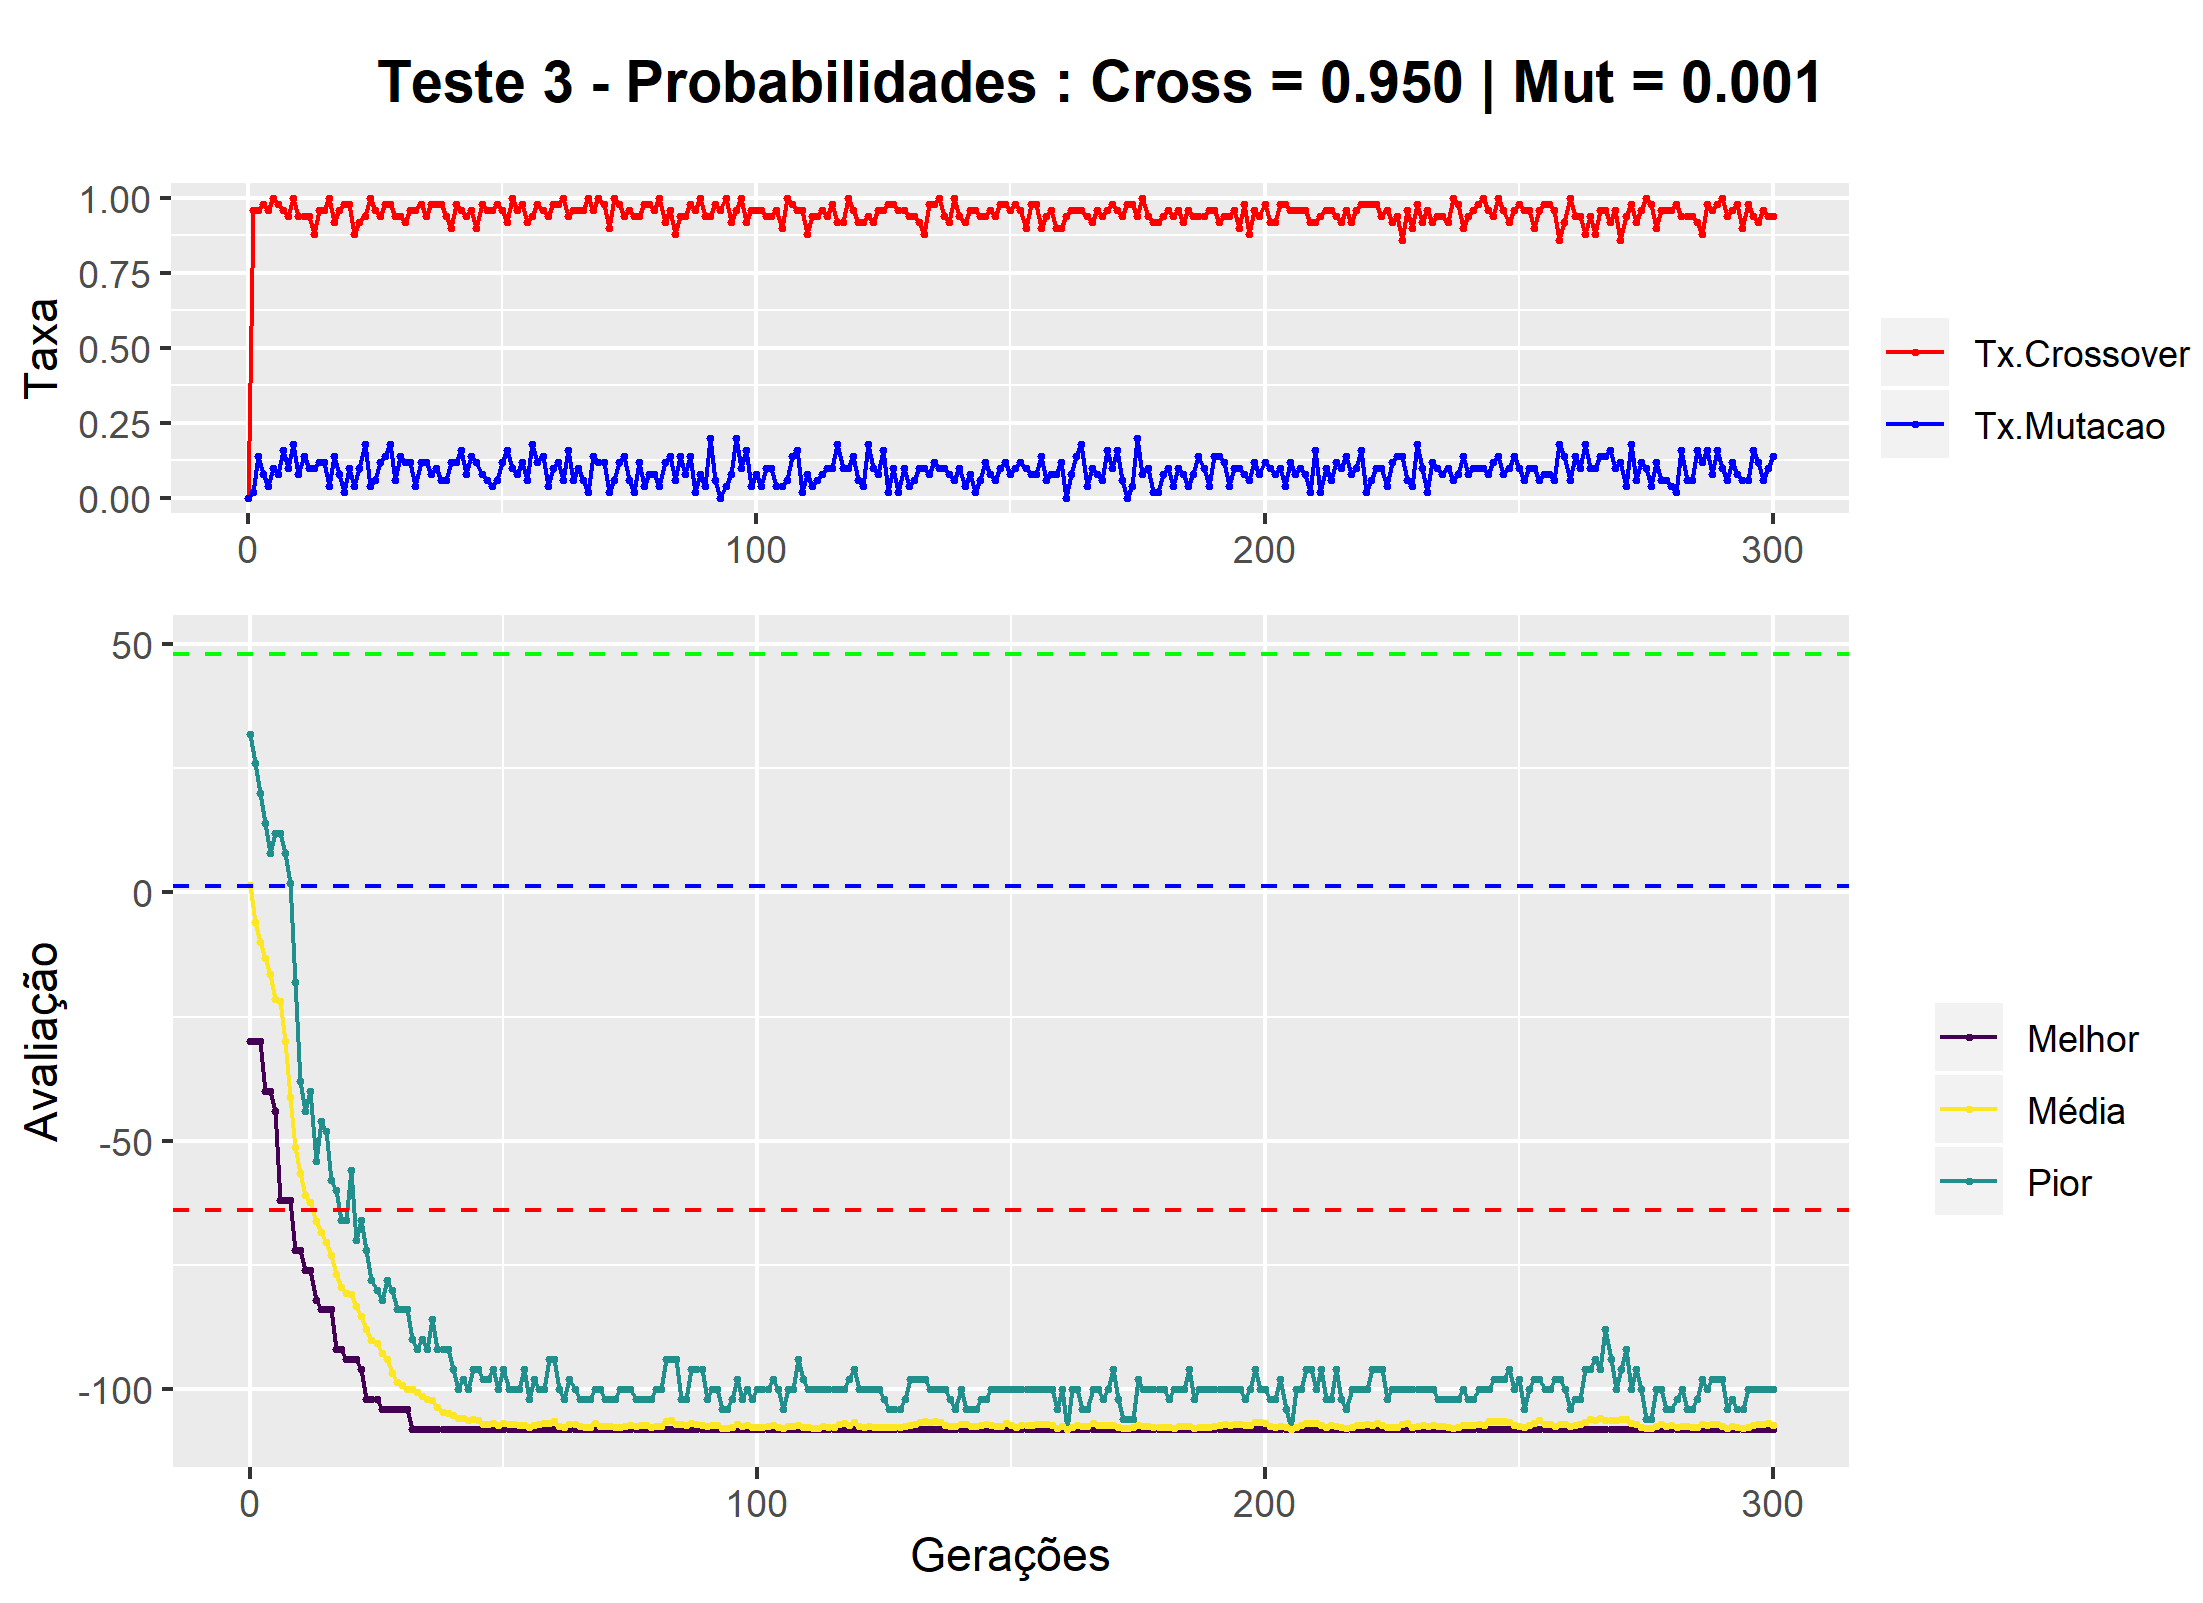
\includegraphics[width=\linewidth]{imagens/graph_pc_0_950_pm_0_001_pop_50_g_300__3.png}
		\caption{}
	\end{subfigure}
	\begin{subfigure}[b]{0.47\linewidth}
		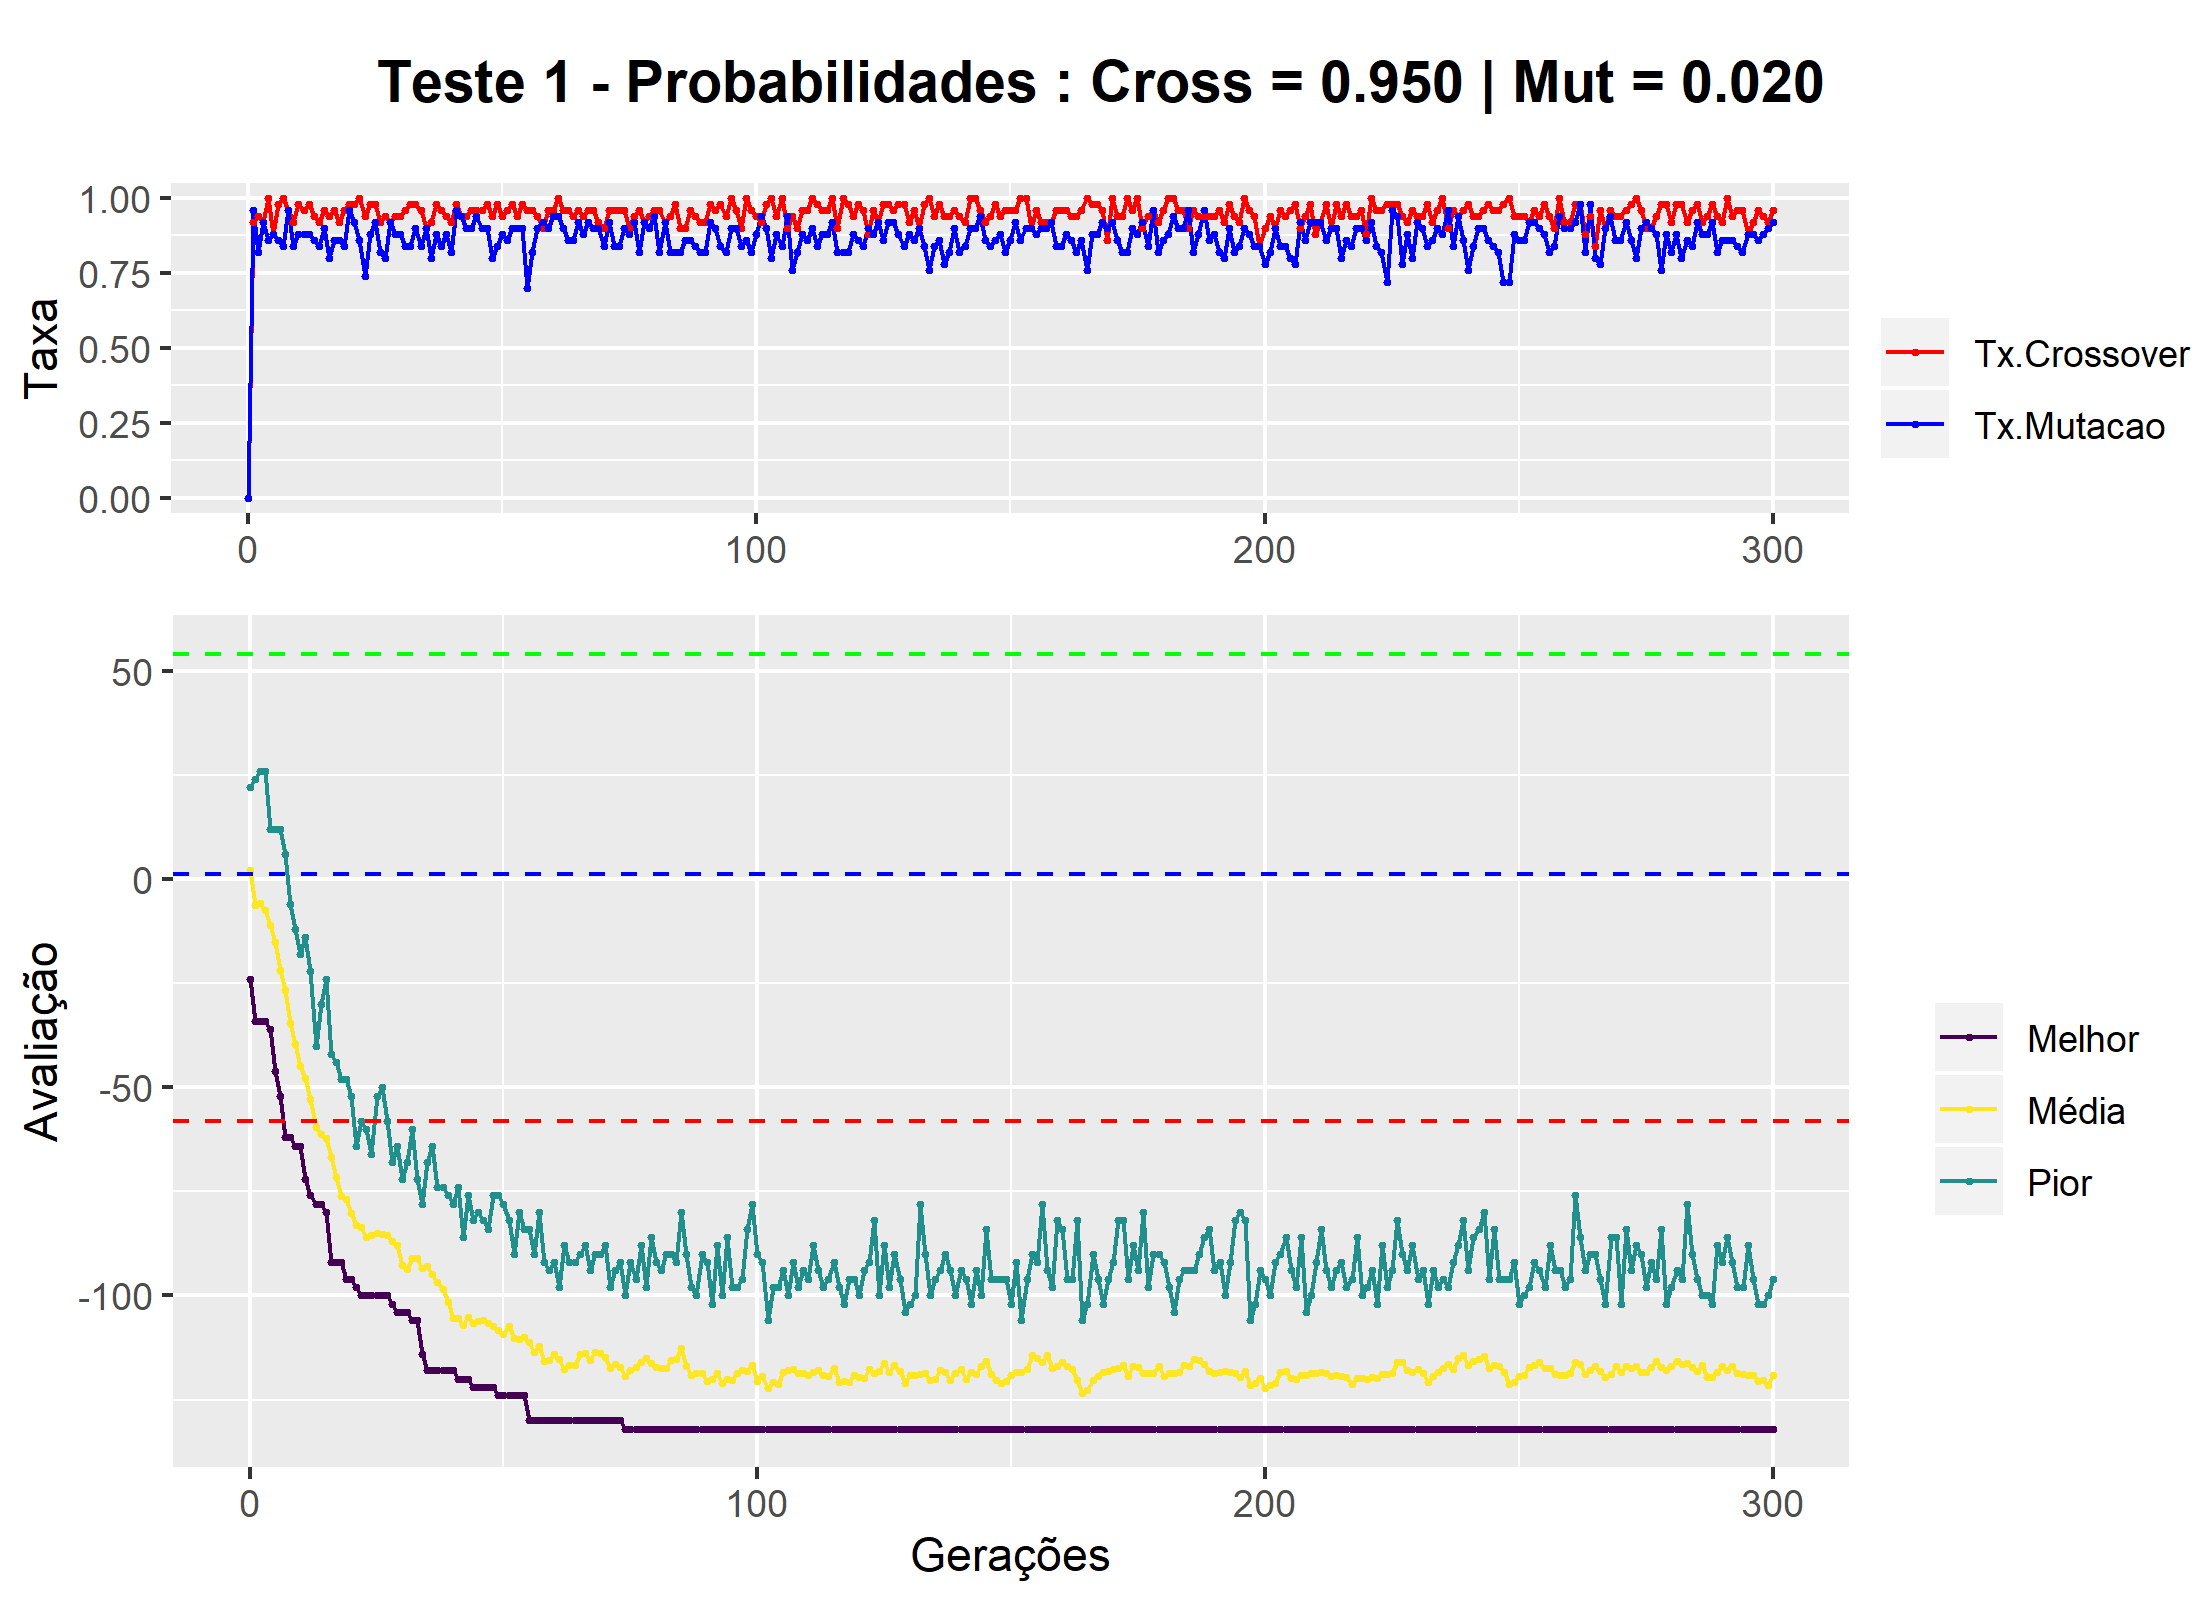
\includegraphics[width=\linewidth]{imagens/graph_pc_0_950_pm_0_020_pop_50_g_300__1.png}
		\caption{}
	\end{subfigure}
	\begin{subfigure}[b]{0.47\linewidth}
		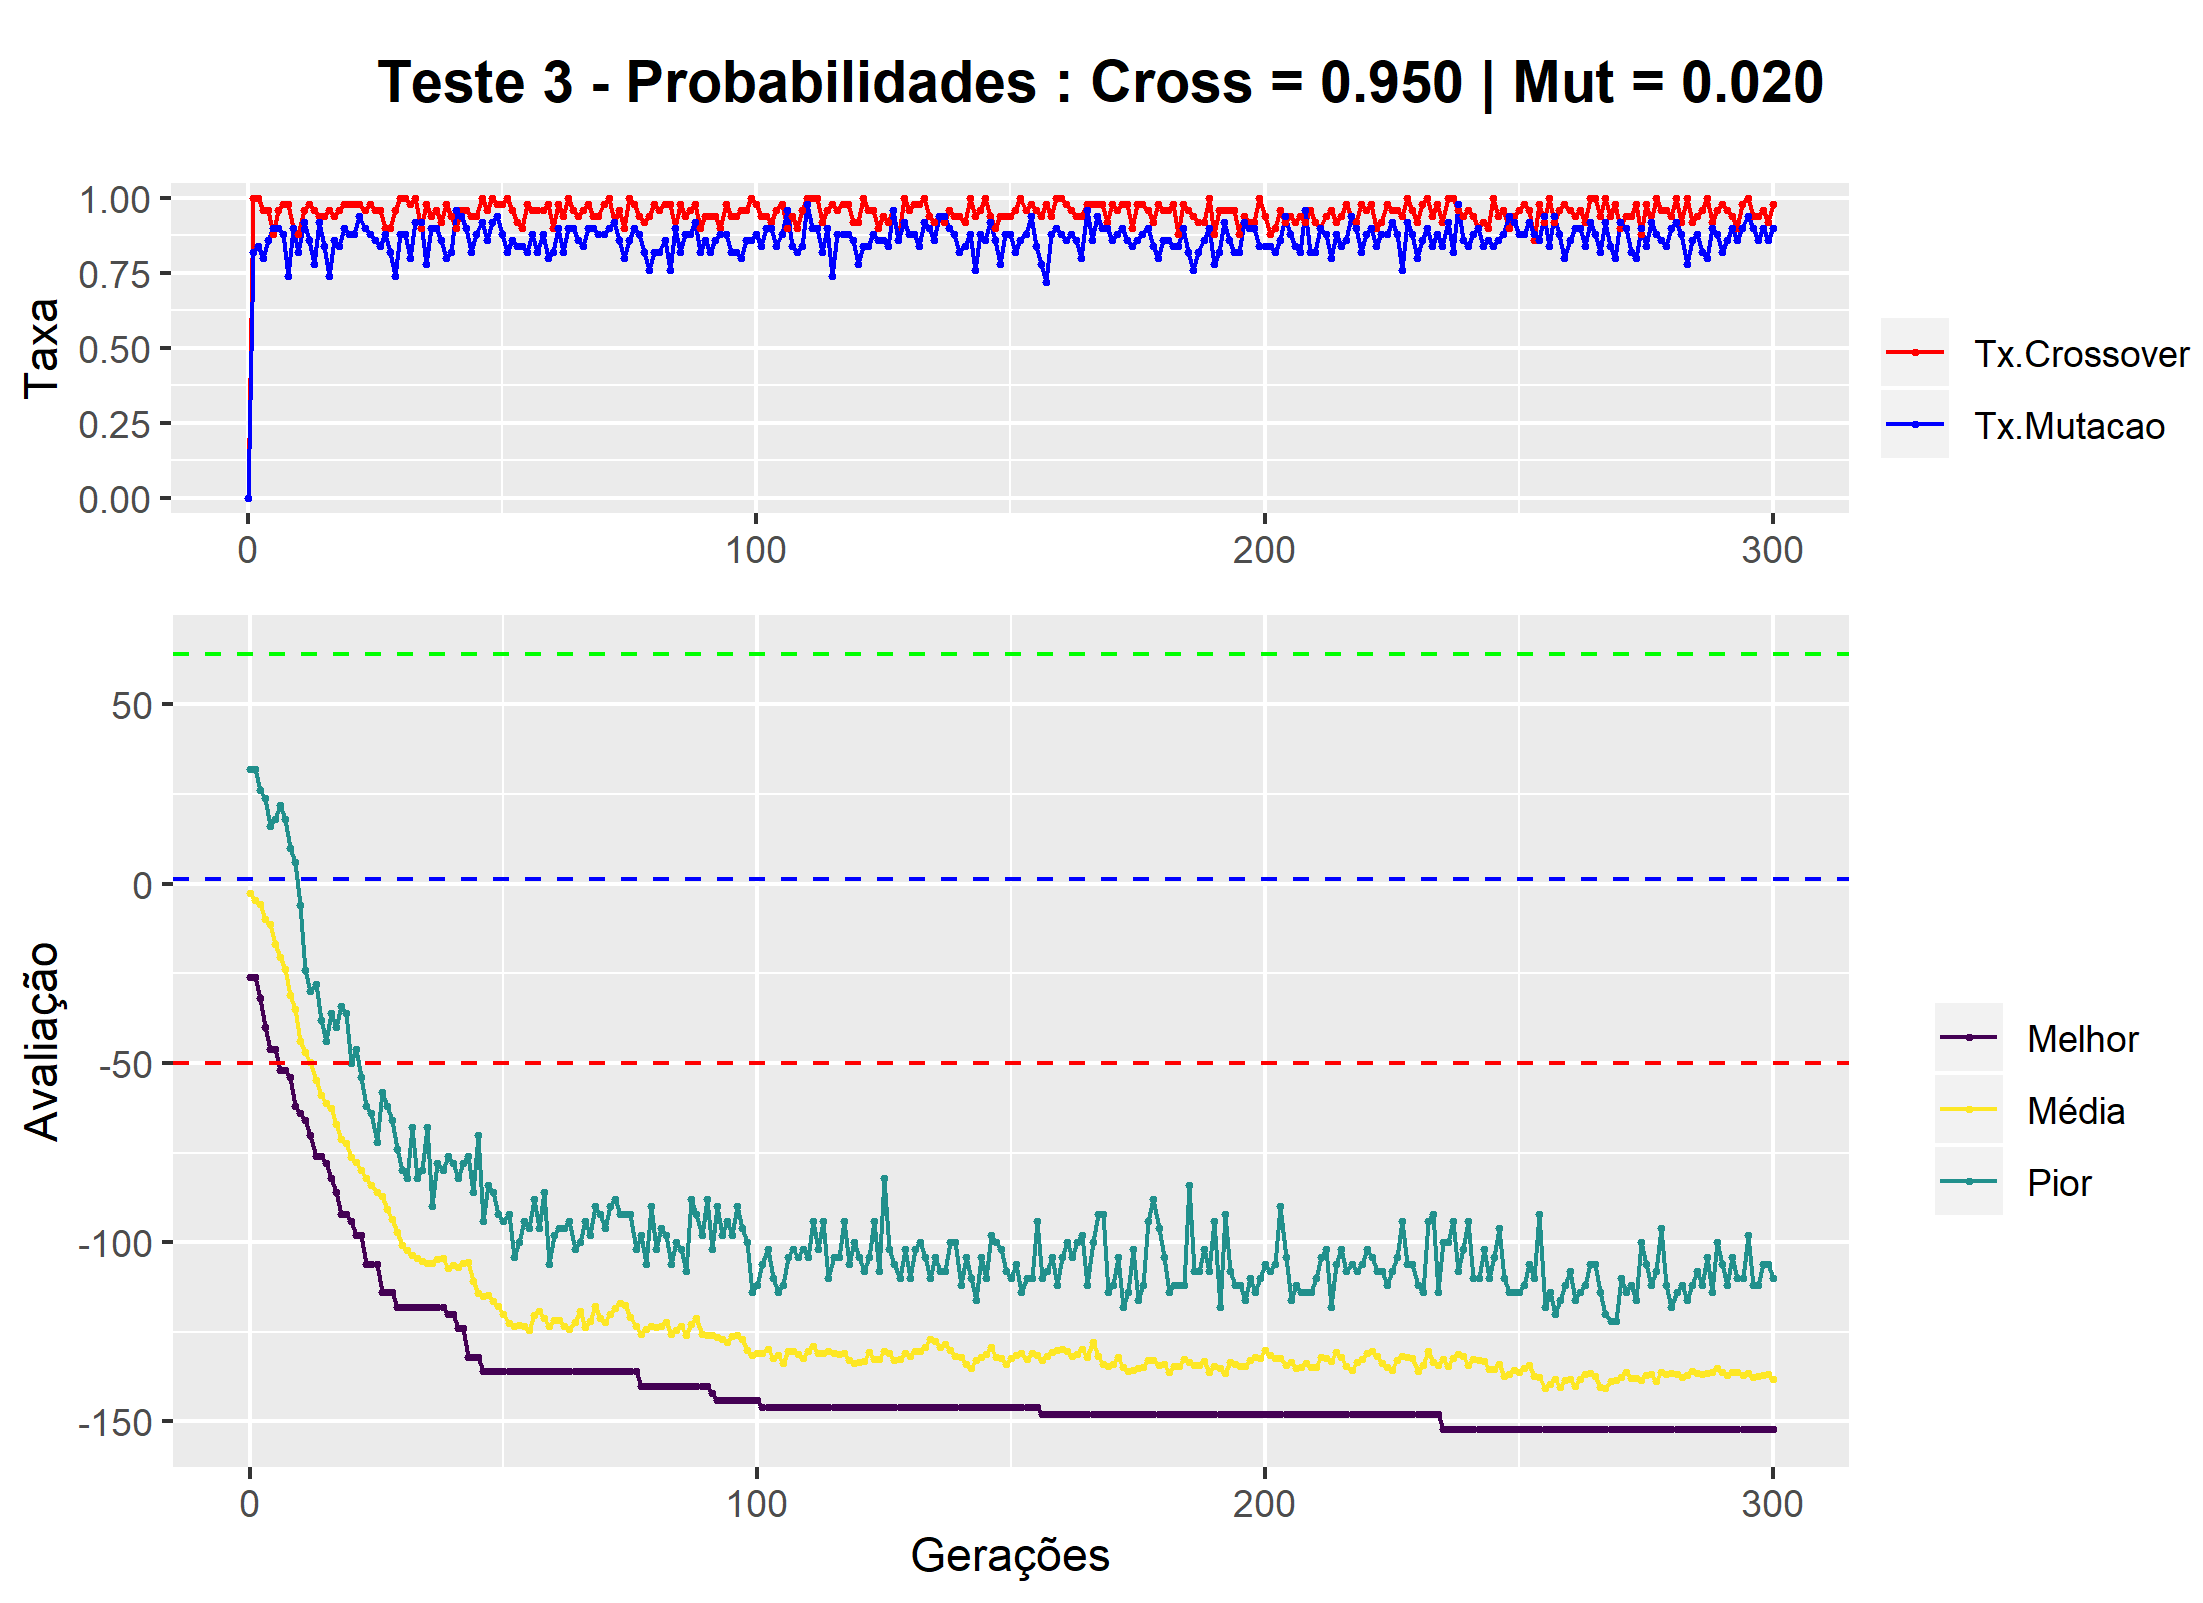
\includegraphics[width=\linewidth]{imagens/graph_pc_0_950_pm_0_020_pop_50_g_300__3.png}
		\caption{}
	\end{subfigure}
	\begin{subfigure}[b]{0.47\linewidth}
		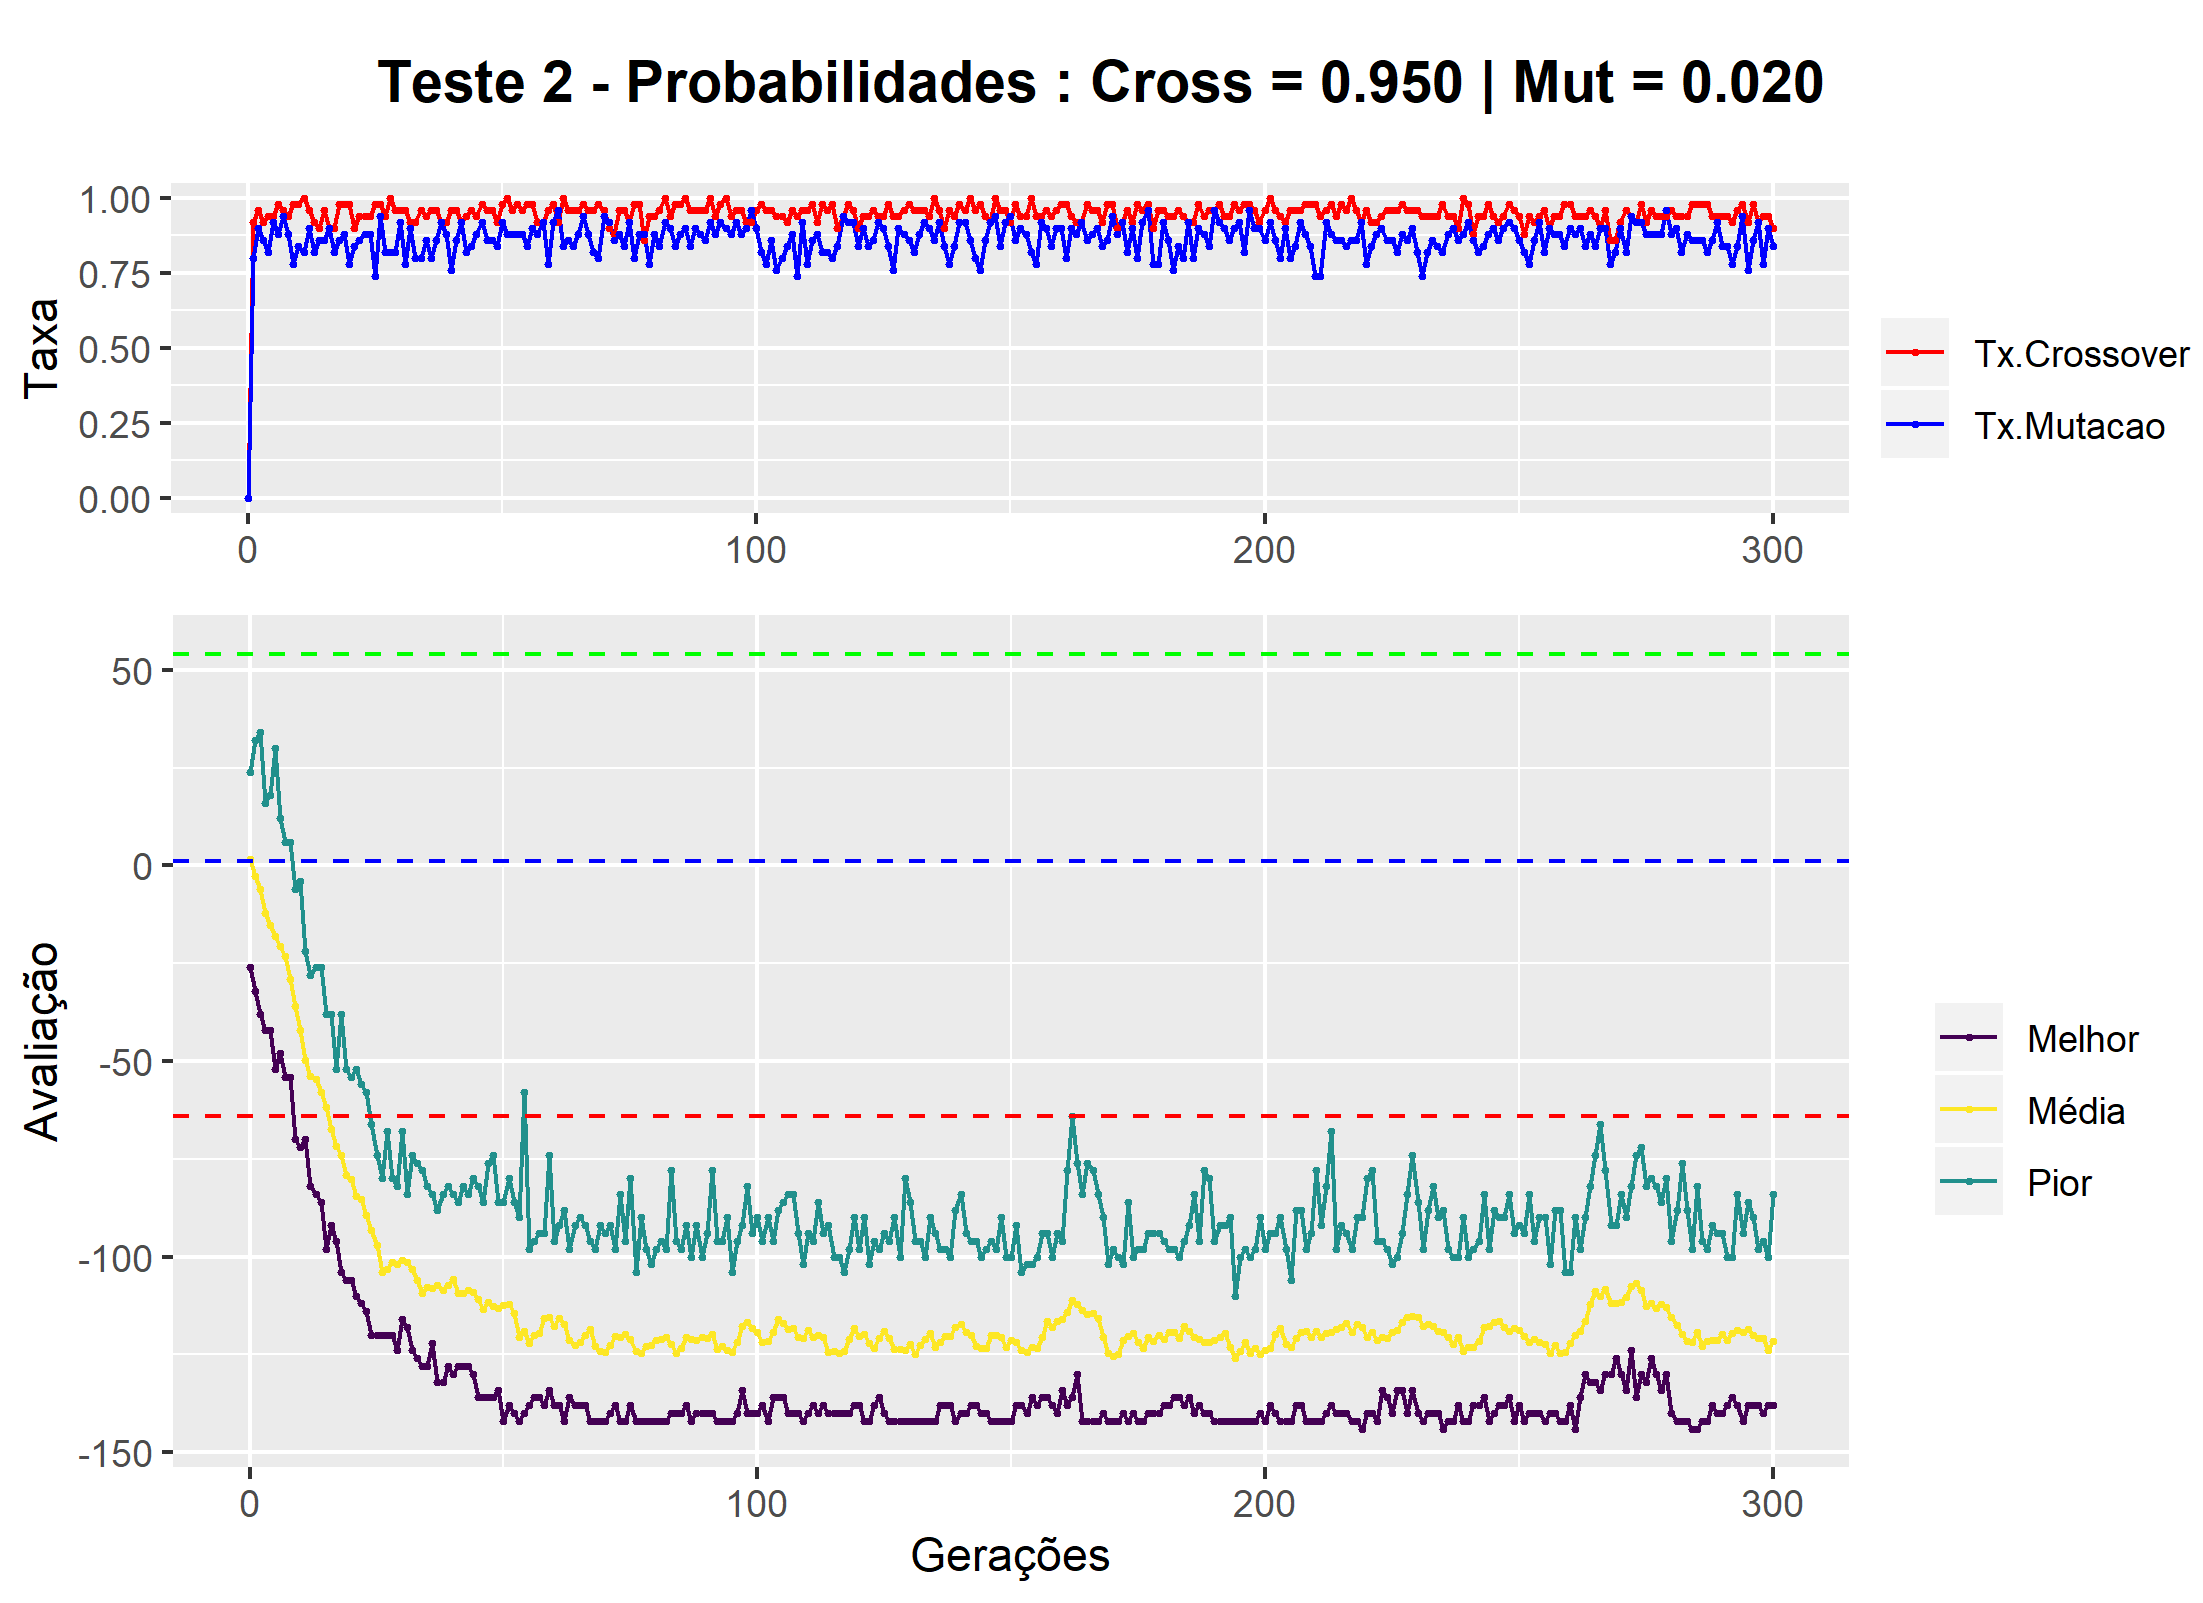
\includegraphics[width=\linewidth]{imagens/graph_pc_0_950_pm_0_020_pop_50_g_300__2_noelite.png}
		\caption{Sem elitismo}
	\end{subfigure}
	\begin{subfigure}[b]{0.47\linewidth}
		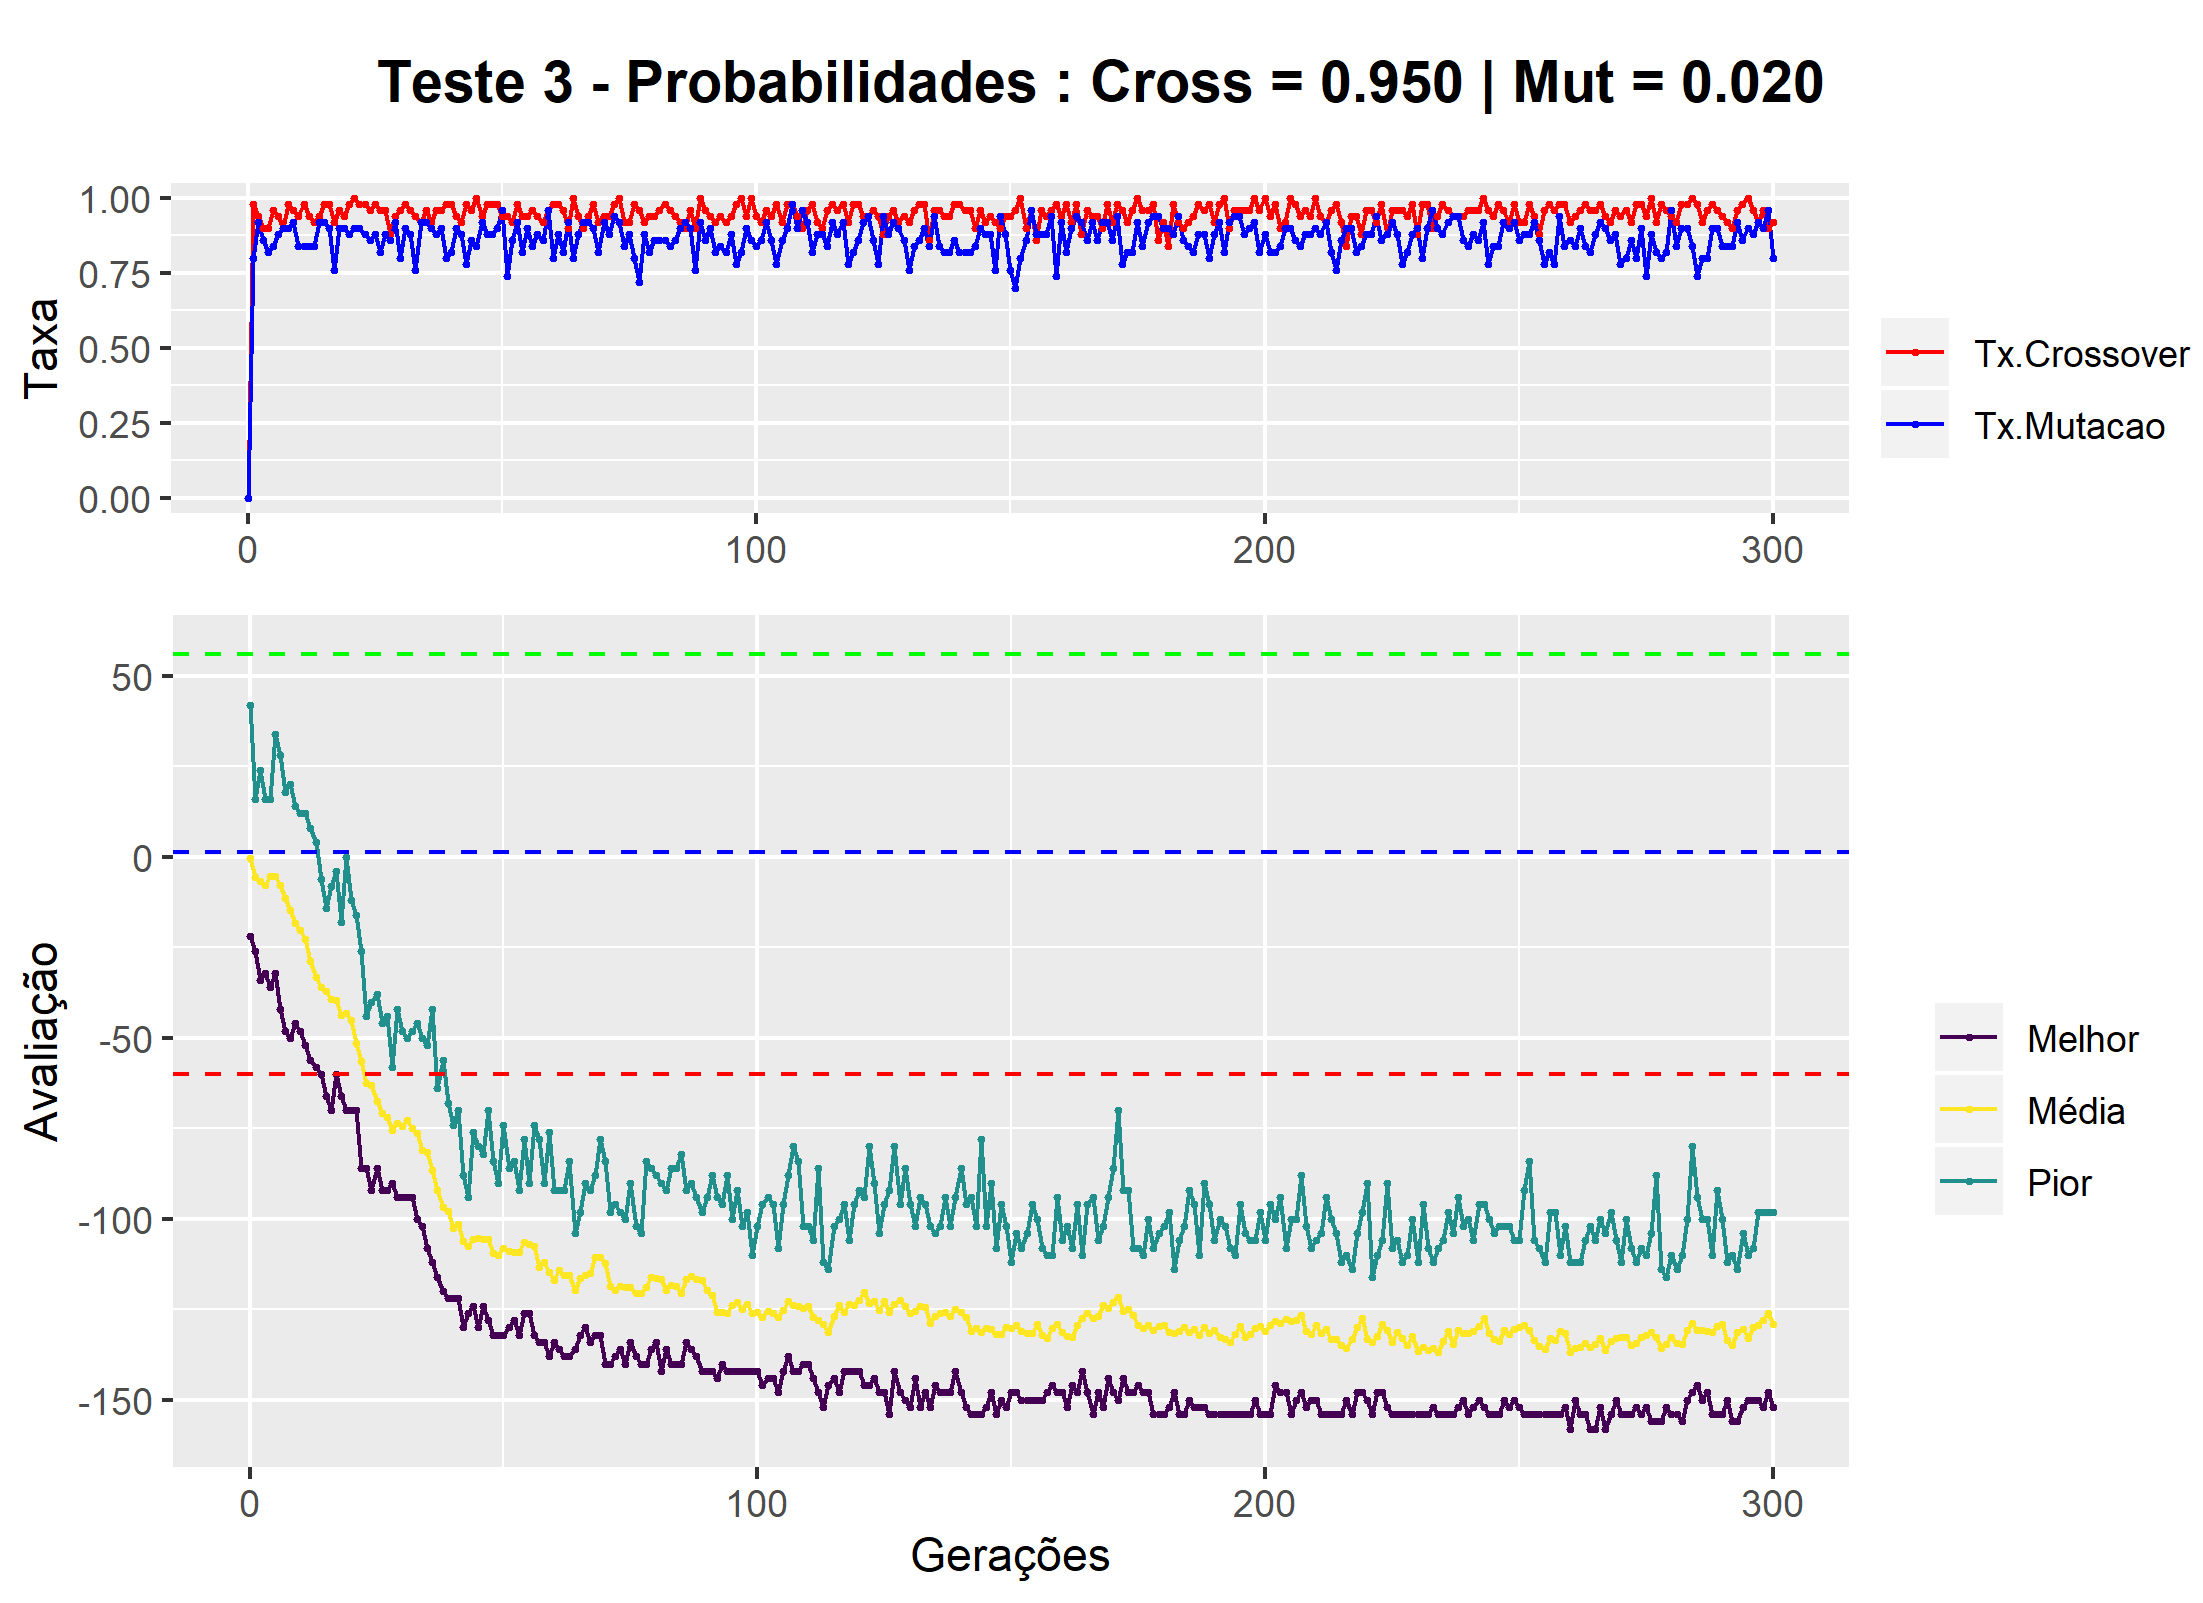
\includegraphics[width=\linewidth]{imagens/graph_pc_0_950_pm_0_020_pop_50_g_300__3_noelite.png}
		\caption{Sem elitismo}
	\end{subfigure}
	\caption{Evolução do algoritmo genético durante gerações}
	\label{fig:evolucaoGA2}
\end{figure}
\clearpage



	\begin{lstlisting}[caption={Resultado de um ciclo de seleção, crossover e mutação do GA para o modelo de Ising}, label=qd:resultado_reproducao_ising] 
Geração: 1 | Média Avaliação: 1.601593
#### CHILD #####
ID: 54
Fenotipo: 
1 | -1 |  1 | -1 | -1 |  1 |  1 | -1 | -1 |  1
--------------------------------------------------
1 |  1 |  1 | -1 | -1 |  1 |  1 | -1 | -1 |  1
--------------------------------------------------
1 |  1 | -1 | -1 |  1 |  1 |  1 |  1 | -1 |  1
--------------------------------------------------
1 |  1 | -1 | -1 |  1 | -1 |  1 |  1 |  1 | -1
--------------------------------------------------
1 |  1 | -1 |  1 | -1 | -1 |  1 |  1 |  1 | -1
--------------------------------------------------
1 |  1 | -1 | -1 | -1 | -1 |  1 |  1 |  1 | -1
--------------------------------------------------
1 |  1 | -1 |  1 | -1 | -1 |  1 |  1 |  1 |  1
--------------------------------------------------
1 |  1 |  1 | -1 | -1 |  1 |  1 |  1 |  1 |  1
--------------------------------------------------
-1 |  1 | -1 | -1 |  1 | -1 | -1 | -1 |  1 | -1
--------------------------------------------------
1 | -1 | -1 |  1 |  1 |  1 | -1 |  1 |  1 |  1

#1:  60 | #-1:  40

Avaliação: 6.685894
#### PARENT 1 #####
ID: 11
Fenotipo: 
1 | -1 | -1 | -1 | -1 | -1 |  1 | -1 | -1 |  1
--------------------------------------------------
-1 |  1 |  1 | -1 | -1 |  1 |  1 | -1 | -1 | -1
--------------------------------------------------
1 |  1 | -1 | -1 | -1 |  1 |  1 |  1 | -1 |  1
--------------------------------------------------
1 |  1 |  1 |  1 |  1 |  1 |  1 | -1 |  1 | -1
--------------------------------------------------
-1 |  1 | -1 |  1 | -1 | -1 | -1 |  1 |  1 | -1
--------------------------------------------------
1 |  1 |  1 | -1 | -1 | -1 |  1 |  1 |  1 | -1
--------------------------------------------------
1 | -1 | -1 |  1 |  1 | -1 | -1 |  1 |  1 |  1
--------------------------------------------------
1 | -1 | -1 | -1 | -1 |  1 |  1 | -1 |  1 | -1
--------------------------------------------------
-1 |  1 | -1 | -1 |  1 | -1 | -1 | -1 |  1 | -1
--------------------------------------------------
1 | -1 | -1 |  1 |  1 |  1 |  1 |  1 |  1 |  1

#1:  52 | #-1:  48

Avaliação: 1.000000
Selecionado 2 vezes, 0.04

#### PARENT 2 #####
ID: 13
Fenotipo: 
1 |  1 |  1 | -1 | -1 |  1 |  1 | -1 |  1 |  1
--------------------------------------------------
1 |  1 |  1 |  1 | -1 |  1 | -1 | -1 | -1 |  1
--------------------------------------------------
-1 |  1 |  1 |  1 |  1 |  1 | -1 | -1 | -1 |  1
--------------------------------------------------
-1 | -1 | -1 | -1 |  1 | -1 |  1 | -1 | -1 | -1
--------------------------------------------------
1 | -1 | -1 | -1 | -1 | -1 |  1 | -1 | -1 | -1
--------------------------------------------------
-1 |  1 | -1 |  1 | -1 |  1 |  1 | -1 | -1 | -1
--------------------------------------------------
1 |  1 | -1 | -1 | -1 | -1 |  1 |  1 |  1 | -1
--------------------------------------------------
1 | -1 |  1 |  1 |  1 |  1 |  1 |  1 |  1 |  1
--------------------------------------------------
-1 | -1 | -1 | -1 |  1 | -1 | -1 |  1 |  1 | -1
--------------------------------------------------
1 |  1 | -1 |  1 |  1 |  1 | -1 |  1 |  1 |  1

#1:  52 | #-1:  48

Avaliação: 4.055200
Selecionado 11 vezes, 0.22

### HERITAGE MAP ###
2 |  1 |  2 |  1 |  1 |  2 |  1 |  2 |  1 |  2
--------------------------------------------------
2 |  1 |  1 |  1 |  2 |  1 |  1 |  1 |  2 |  2
--------------------------------------------------
1 |  1 |  1 |  1 |  2 |  2 |  1 |  1 |  2 |  1
--------------------------------------------------
1 |  1 |  2 |  2 |  2 |  2 |  2 |  2 |  1 |  1
--------------------------------------------------
2 |  1 |  1 |  1 |  2 |  2 |  2 |  1 |  1 |  1
--------------------------------------------------
1 |  2 |  2 |  1 |  1 |  1 |  2 |  1 |  1 |  2
--------------------------------------------------
1 |  2 |  2 |  1 |  2 |  2 |  2 |  2 |  1 |  1
--------------------------------------------------
2 |  1 |  2 |  1 |  1 |  2 |  2 |  2 |  2 |  2
--------------------------------------------------
2 |  1 |  2 |  2 |  1 |  1 |  1 |  1 |  1 |  1
--------------------------------------------------
1 |  1 |  2 |  2 |  1 |  2 |  2 |  1 |  2 |  2

### MUTATE MAP
FA | FA | FA | FA | FA | FA | FA | FA | FA | FA
--------------------------------------------------
FA | FA | FA | FA | FA | FA | FA | FA | FA | FA
--------------------------------------------------
FA | FA | FA | FA | FA | FA | FA | FA | FA | FA
--------------------------------------------------
FA | FA | FA | FA | FA | FA | FA | TR | FA | FA
--------------------------------------------------
FA | FA | FA | FA | FA | FA | FA | FA | FA | FA
--------------------------------------------------
FA | FA | FA | FA | FA | FA | FA | FA | FA | FA
--------------------------------------------------
FA | FA | FA | FA | FA | FA | FA | FA | FA | FA
--------------------------------------------------
FA | TR | FA | FA | FA | FA | FA | FA | FA | FA
--------------------------------------------------
FA | FA | FA | FA | FA | FA | FA | FA | FA | FA
--------------------------------------------------
FA | FA | FA | FA | FA | FA | FA | FA | FA | FA
	\end{lstlisting}


%% ---
%\chapter{Morbi ultrices rutrum lorem.}
%% ---
%\lipsum[30]
%
%% ---
%\chapter{Cras non urna sed feugiat cum sociis natoque penatibus et magnis dis
%parturient montes nascetur ridiculus mus}
%% ---
%
%\lipsum[31]
%
%% ---
%\chapter{Fusce facilisis lacinia dui}
%% ---
%
%\lipsum[32]

\end{anexosenv}

%---------------------------------------------------------------------
% INDICE REMISSIVO
%---------------------------------------------------------------------
\phantompart
\printindex
%---------------------------------------------------------------------

\end{document}
